\documentclass{article}
\usepackage[utf8]{inputenc}
\usepackage{amsmath}
\usepackage{amsfonts}
\usepackage{amssymb}
\usepackage{graphicx}
\usepackage{subcaption}
\usepackage{enumitem}
\usepackage{blindtext}
\usepackage{hyperref}

\title{Understanding Analysis 2nd Edition - Stephen Abbott (Notes) \footnote{Recorded lectures that I followed: \url{https://www.youtube.com/playlist?list=PLLFpXNanTP9WGfbjxR5kCMXQgol4bGehz}}}
\author{Zhenyong Shin}
\date{March 2021}

\begin{document}

\maketitle

\section{The Real Numbers}
\subsection{Discussion: The Irrationality of $\sqrt{2}$}
    \fbox{\parbox{\textwidth}{
    \textbf{Theorem 1.1.1.} \textit{Let $\mathbb{Q}$ be the set of all rational numbers. Then $\forall x \in \mathbb{Q}, x^2 \neq 2$.}
    }}\\ \\
    \textit{Proof.} Let $x \in \mathbb{Q}$, then $x = p/q$, where $p,q \in \mathbb{Z}$. By contradiction, suppose
    \begin{equation}
        \exists p,q \in \mathbb{Z}: \bigg( \frac{p}{q} \bigg)^2 = 2.
        \label{(p/q)^=2}
    \end{equation}
    Assume that $p$ and $q$ have no common factor, if they had one, it can be canceled out and $\frac{p}{q}$ can be rewritten in lowest terms. Equation (\ref{(p/q)^=2}) implies that
    \begin{equation}
        p^2 = 2q^2.
        \label{p^2=2q^2}
    \end{equation}
    From equation (\ref{p^2=2q^2}), $p^2$ is an even number. Hence $p$ is an even number since the square of an odd number is odd. Let $p=2r$,
    \begin{gather*}
        (2r)^2 = 4r^2 = 2q^2 \\
        2r^2 = q^2.
    \end{gather*}
    So $q^2$ is even and hence $q$ is even. Thus, $p$ and $q$ are both even (divisible by 2). This contradicts the assumption that they have no common factor. Therefore, equation (\ref{(p/q)^=2}) is false and there is no rational number whose square is 2.\\ \\ 
    QED\\
    
    To strengthen the concept of number, one moves from the rational numbers to a larger number system. Starting with the \textit{natural numbers}
    \begin{equation*}
        \mathbb{N} = \{1,2,3,4,5,\dots\}.
    \end{equation*}
    Addition can be performed perfectly well in $\mathbb{N}$. But to have an additive identity ($a+b=a$) and the additive inverses ($a+b=0$) necessary to define subtraction, the system must be extended to the \textit{integers}
    \begin{equation*}
        \mathbb{Z} = \{\dots, -3, -2, -1, 0, 1, 2, 3, \dots\}.
    \end{equation*}
    The number 1 acts as the multiplication identity ($a \cdot b = a$), but multiplicative inverses ($a \cdot b=1$) are needed to define division. Thus, the system must be extended to the \textit{rational numbers}
    \begin{equation*}
        \mathbb{Q} = \bigg\{ \frac{p}{q}: p,q \in \mathbb{Z}, q \neq 0 \bigg\}.
    \end{equation*}
    
    Taken together, the properties of $\mathbb{Q}$ make up the definition of a \textit{field}. A field is any set where:
    \begin{enumerate}
        \item Addition and multiplication are well-defined operations that are commutative ($a+b=b+a \text{ and }a \cdot b = b \cdot a$), associative ($a+(b+c)=(a+b)+c$ and $a\cdot (b \cdot c) = (a \cdot b) \cdot c$), and obey the distributive property $a(b+c) = ab+ac$. 
        \item There must be an additive identity, and every element must have an additive inverse.
        \item There must be a multiplicative identity, and multiplicative inverses must exist for all nonzero elements of the field.
    \end{enumerate}
    The set $\mathbb{Q}$ also has a natural \textit{order} defined on it. If $r,s \in \mathbb{Q}$, then either
    \begin{equation*}
        r < s, \text{ } r=s, \text{ or } r > s.
    \end{equation*}
    This ordering is transitive in the sense that if $r < s$ and $s < t$, then $r < t$, leading to a mental picture of the rational numbers as being laid out from left to right along a number line. 
    
    Unlike $\mathbb{Z}$, there are no intervals of empty space. If $r, s \in \mathbb{Q}$, where $r < s$, then $(r+s)/2$ sits halfway in between, implying that the rational numbers are densely nestled together.
    
    The rational numbers can approximate $\sqrt{2}$ quite well. For instance, $1.414^2 = 1.999396$. By adding more decimal places to the approximation, one can get even closer to a value for $\sqrt{2}$ (Figure \ref{approx. sqrt2}). Even so, there is a “hole” in the rational number line where $\sqrt{2}$ ought to be (among others such as $\sqrt{3}$ and $\sqrt{5}$). Thus, to the chain $\mathbb{N} \subseteq \mathbb{Z} \subseteq \mathbb{Q}$ one appends the \textit{real numbers} $\mathbb{R}$.\\
    \begin{figure}[ht!]
        \centering
        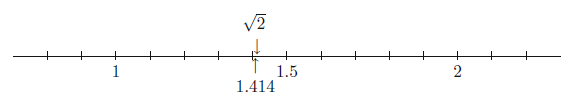
\includegraphics[width=0.9\textwidth]{figs/approx. sqrt2.png}
        \caption{Approximating $\sqrt{2}$ with rational numbers}
        \label{approx. sqrt2}
    \end{figure}
    How to construct $\mathbb{R}$ from $\mathbb{Q}$ is complicated. For now, assume that $\mathbb{R}$ is obtained by filling in the "holes" in $\mathbb{Q}$. Wherever there is a hole, a new irrational number $i \in \mathbb{I}$ is defined and placed into the ordering that already exists on $\mathbb{Q}$. $\mathbb{R}$ is then the union of these irrational numbers  together with the rational ones, $\mathbb{R} = \mathbb{I} \cup \mathbb{Q}$.

\subsection{Some Preliminaries}
\subsubsection{Sets}
    A \textit{set} is any collection of objects. The objects in a set are the \textit{elements} of the set. Given a set $A$, if $x$ is an elements of $A$, then $x \in A$. Otherwise, $x \notin A$. Given two sets $A$ and $B$, their
    \begin{enumerate}
        \item \textit{Union} is the set $A \cup B$ and $x \in A \cup B$ if $x \in A$ or $x \in B$ or both.
        \item \textit{Intersection} is the set $A \cap B$ and $x \in A \cap B$ provided $x \in A$ and $x \in B$. 
    \end{enumerate}
    The \textit{empty set} $\emptyset$ is a set that contains no elements. If $A \cap B = \emptyset$, then $A$ and $B$ are \textit{disjoint}.
    
    The \textit{inclusion} relationship $A \subseteq B$ or $B \supseteq A$ indicates that $x \in A \implies x \in B$. In this case, $A$ is a \textit{subset} of $B$, or $B$ \textit{contains} $A$. If $A \subseteq B$ and $B \subseteq A$, then $A = B$. Let 
    \begin{align*}
        A_1 & = \mathbb{N} = \{1,2,3,\dots\}, \\
        A_2 & = \{2,3,4,\dots\}, \\
        A_3 & = \{3,4,5,\dots\}, \\
        & \vdots
        \\
        A_n & = \{n, n+1, n+2, \dots\}.
    \end{align*}
    The result is a nested chain of sets $A_1 \supseteq A_2 \supseteq A_3 \supseteq A_4 \supseteq \dots$, where each successive set is a subset of all the previous ones. Notationally,
    \begin{equation*}
        \bigcup_{n=1}^\infty A_n, \text{ } \bigcup_{n \in \mathbb{N}} A_n, \text{ or } A_1 \cup A_2 \cup \dots
    \end{equation*}
    are all equivalent ways to indicate the set whose elements consists of any element that appears in at least one particular $A_n$. Because of the nested property of this particular collection of sets,
    \begin{equation*}
        \bigcup_{n=1}^\infty A_n = A_1.
    \end{equation*}
    The notion of intersection has the same kind of natural extension to infinite collections of sets. For this example,
    \begin{equation*}
        \bigcap_{n=1}^\infty A_n = \emptyset.
    \end{equation*}
    Suppose there is some natural number $m \in \cap_{n=1}^\infty A_n$. So $m \in A_n$ for every $A_n$. Because $m$ is not an element of $A_{m+1}$, no such $m$ exists and the intersection is empty. Given $A \subseteq \mathbb{R}$, the \textit{complement} of $A$ is
    \begin{equation*}
        A^c = \{x \in \mathbb{R}: x \notin A\}.
    \end{equation*}\\
    \fbox{\parbox{\linewidth}{\textbf{De Morgan's Laws:} (i) $(A \cap B)^c = A^c \cup B^c$ and (ii) $(A \cup B)^c = A^c \cap B^c$.}} 
    \\ \\
    \textit{Proof.} (i) Let $x \in (A \cap B)^c$, then $x \notin A \cap B$. This means $x \notin A$ or $x \notin B$, so $x \in A^c$ or $x \in B^c$. Hence, $x \in A^c \cup B^c$. This means that $(A \cap B)^c \subseteq A^c \cup B^c$.
    
    Now let $x \in A^c \cup B^c$. Then $x \in A^c$ or $x \in B^c$, so $x \notin A$ or $x \notin B$. This means that $x \notin A \cap B$. Hence, $x \in (A \cap B)^c$. This means that $A^c \cup B^c \subseteq (A \cap B)^c$.
    
    Since $(A \cap B)^c \subseteq A^c \cup B^c$ and $A^c \cup B^c \subseteq (A \cap B)^c$, therefore $(A \cap B)^c = A^c \cup B^c$.
    \\ \\
    (ii) Let $x \in (A \cup B)^c$, so $x \notin A \cup B$. This means that $x \in A^c$ and $x \in B^c$. Hence, $x \in A^c \cap B^c$. This means that $(A \cup B)^c \subseteq A^c \cap B^c$.
    
    Now let $x \in A^c \cap B^c$. So $x \in A^c$ and $x \in B^c$, which means $x \notin A$ and $x \notin B$. This means that $x \notin A \cup B$. Hence, $x \in (A \cup B)^c$. This means that $A^c \cap B^c \subseteq (A \cup B)^c$.
    
    Since $(A \cup B)^c \subseteq A^c \cap B^c$ and $A^c \cap B^c \subseteq (A \cup B)^c$, therefore $(A \cup B)^c = A^c \cap B^c$.\\ \\
    QED

\subsubsection{Functions}
        \fbox{\parbox{\linewidth}{\textbf{Definition 1.2.3.} Given two sets $A$ and $B$, a \textit{function} $f: A \to B$ is a rule or mapping that takes each element $x \in A$ and associates with it a single element of $B$. Given $x \in A$, $f(x)$ represents the element of $B$ associated with $x$ by $f$. The set $A$ is the \textit{domain} of $f$. The \textit{range} of $f$ is not necessarily $B$ but the subset of $B$ given by $\{y \in B: y=f(x),x\in A\}$.}}
        \\ \\
        \textbf{Example 1.2.4.} In 1829, Peter Lejeune Dirichlet proposed the unruly function
        \begin{equation*}
            g(x) = \bigg\{ \begin{matrix}1 & \text{if } x \in \mathbb{Q} \\ 0 & \text{ if } x \notin \mathbb{Q}. \end{matrix}
        \end{equation*}
        The domain of $g$ is $\mathbb{R}$, and the range is $\{0,1\}$. There is no single formula for $g$ in the usual sense, and it is quite difficult to graph this function, but it certainly qualifies as a function according to Definition 1.2.3.\\ \\
        \textbf{Example 1.2.5.} The \textit{absolute value function} is defined as
        \begin{equation*}
            |x| = \bigg\{ \begin{matrix}x, & x \geq 0 \\ -x, & x<0.\end{matrix}
        \end{equation*}
        With respect to multiplication and division, the absolute value function satisfies
        \begin{enumerate}
            \item $|ab| = |a||b|$
            \item $|a+b| \leq |a| + |b|$ (\textit{Triangle inequality})
            \item $|a-b| \geq |a| - |b|$ (\textit{Reverse Triangle Inequality})
        \end{enumerate}
        for all choices of $a$ and $b$. Given three real numbers $a,b, \text{and } c$,
        \begin{equation*}
            |a - b| = |(a - c) + (c - b)|.
        \end{equation*}
        By the triangle inequality,
        \begin{equation*}
            |(a - c) + (c - b)| \leq |a - c| + |c - b|,
        \end{equation*}
        so
        \begin{equation}
            |a - b| \leq |a - c| + |c - b|.
        \end{equation}
    
    \subsubsection{Logic and Proofs}
        \fbox{\parbox{\linewidth}{\textbf{Theorem 1.2.6.} \textit{Two real numbers a and b are equal if and only if for every real number $\epsilon > 0$ it follows that $|a - b| < \epsilon$.}}}
        \\ \\ 
        \textit{Proof.} Logically,
        \begin{equation*}
            a,b \in \mathbb{R}: a=b \iff \forall \epsilon \in \mathbb{R}, \epsilon > 0, |a-b|<\epsilon.
        \end{equation*}
        $(\Rightarrow)$ Let $a,b \in \mathbb{R}, a=b$. Then $|a-b|=0$, so $\forall \epsilon \in \mathbb{R}, \epsilon > 0, |a-b| = 0 <\epsilon$.
        \\ \\
        $(\Leftarrow)$ Let $\forall \epsilon \in \mathbb{R}, \epsilon > 0, |a-b|<\epsilon$. By contradiction, assume that $a \neq b$. So,
        \begin{equation*}
            \exists \epsilon \in \mathbb{R}, \epsilon > 0: |a-b| = \epsilon.
        \end{equation*}
        But this contradicts that $|a-b| < \epsilon$. Hence $a \neq b$ is false and $a=b$. \\ \\
        QED
    
    \subsubsection{Induction}
        Induction is used together with $\mathbb{N}$ (or sometimes $\mathbb{N} \cup \{0\}$). The fundamental principle behind induction is that if $S \subseteq \mathbb{N}$ with the properties that
        \begin{enumerate}
            \item $1 \in S$
            \item If $n \in S$, then $n+1 \in S$,
        \end{enumerate}
        then it must be that $S = \mathbb{N}$.\\ \\
        \textbf{Example 1.2.7.} Let $x_1 = 1$, and for each $n \in \mathbb{N}$ define
        \begin{equation*}
            x_{n+1} = \frac{1}{2}x_n + 1.
        \end{equation*}
        Using this rule, $x_2 = (1/2)(1)+1 = 3/2, x_3 = 7/4$, and this leads to a definition of $x_n$ for $\forall n \in \mathbb{N}$. \\ \\
        For the first few terms, it is true that $x_1 \leq x_2 \leq x_3$. Let's use induction to prove that 
        \begin{equation}
            x_n \leq x_{n+1}
            \label{x_n leq x_n+1}
        \end{equation}
        for $\forall n \in \mathbb{N}$. Now, show that
        \begin{equation*}
            \text{if $x_n \leq x_{n+1}$, then $x_{n+1} \leq x_{n+2}$.}
        \end{equation*}
        Let $S$ be the set of natural numbers for which equation (\ref{x_n leq x_n+1}) is true. For $n=1$, $x_1 = 1$ and $x_2 = 3/2$, so $x_1 \leq x_2$. Hence $1 \in S$. Now show that if $n \in S$, then $n+1 \in S$ as well. Assume that for $n \in \mathbb{N}$, $x_n \leq x_{n+1}$ is true, so $n \in S$. To prove $x_{n+1} \leq x_{n+2}$, multiply the inequality by $1/2$ and add 1,
        \begin{align*}
             \frac{1}{2}x_n + 1 & \leq \frac{1}{2}x_{n+1} + 1 \\
            \therefore x_{n+1} & \leq x_{n+2}.
        \end{align*}
        So $n+1 \in S$ as well. By induction, equation (\ref{x_n leq x_n+1}) is proved for all $n \in \mathbb{N}$.
    
    \subsection{The Axiom of Completeness}
    \subsubsection{An Initial Definition for R}
        Assume that:
        \begin{enumerate}
            \item $\mathbb{R}$ is a set containing $\mathbb{Q}$. The operations of addition and multiplication on $\mathbb{Q}$ extend to all of $\mathbb{R}$ such that every element of $\mathbb{R}$ has an additive inverse and every nonzero element of $\mathbb{R}$ has a multiplicative inverse.
            \item $\mathbb{R}$ is a field. The addition and multiplication of real numbers are commutative, associative, and the distributive property holds.
            \item The properties of the ordering on $\mathbb{Q}$ extend to all of $\mathbb{R}$. For example, for $a,b,c \in \mathbb{R}$ if $a < b$ and $c > 0$, then $ac < bc$.
            \item $\mathbb{R}$ is an ordered field , which contains $\mathbb{Q}$ as a subfield.
        \end{enumerate}
        \fbox{\parbox{\linewidth}{\textbf{Axiom of Completeness.} \textit{Every nonempty set of real numbers that is bounded above has a least upper bound.}}}
    
    \subsubsection{Least Upper Bounds and Greatest Lower Bounds}
        \fbox{\parbox{\linewidth}{\textbf{Definition 1.3.1.} A set $A \subseteq \mathbb{R}$ is:
        \begin{enumerate}
            \item \textit{bounded above} if $\exists b \in \mathbb{R}: \forall a \in A, a \leq b$. The number $b$ is called an \textit{upper bound} for $A$.
            \item \textit{bounded below} if $\exists l \in \mathbb{R}: \forall a \in A, l \leq A$. The number $l$ is called a \textit{lower bound} for $A$.
        \end{enumerate}}}
        
        \fbox{\parbox{\linewidth}{\textbf{Definition 1.3.2.} A real number $s \in \mathbb{R}$ is the
        \begin{enumerate}
            \item \textit{least upper bound/supremum} for a set $A \subseteq \mathbb{R}$ (written $s = \sup A$) if:
                \begin{enumerate}
                    \item $s$ is an upper bound for $A$.
                    \item If $b$ is any upper bound for $A$, then $s \leq b$.
                \end{enumerate}
            \item \textit{greatest lower bound/infimum} for a set $A \subseteq \mathbb{R}$ (written $s = \inf A$) if:
                \begin{enumerate}
                    \item $s$ is an lower bound for $A$.
                    \item If $l$ is any lower bound for $A$, then $s \geq l$.
                \end{enumerate}
        \end{enumerate}}}
        
        \begin{figure}[ht!]
            \centering 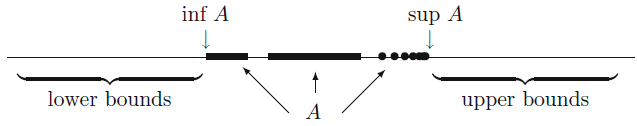
\includegraphics[width=0.9\linewidth]{figs/infsup.png}
            \caption{Definition of $\sup A$ and $\inf A$.}
            \label{supinfA}
        \end{figure}
        Although a set can have a host of upper bounds, it can have only one least upper bound. If $s_1$ and $s_2$ are both least upper bounds for a set $A$, then by property (b) in Definition 1.3.2, $s_1 \leq s_2$ and $s_2 \leq s_1$. Thus $s_1 = s_2$ and least upper bounds are unique.
        \\ \\
        \textbf{Example 1.3.3.} Let 
        \begin{equation*}
            A = \bigg\{\frac{1}{n}:n \in \mathbb{N}\bigg\} = \bigg\{1,\frac{1}{2},\frac{1}{3},\dots\bigg\}.
        \end{equation*}
        The set A is bounded above and below. Its upper bounds include 3, 2, 3/2, etc. For the least upper bound, by Definition 1.3.2 property (a), observe that $1 \geq 1/n$ for $\forall n \in \mathbb{N}$. For property (b), assume that there exists some other upper bound $b$. Because $1 \in A$ and $b$ is an upper bound for $A$, it must be that $1 \leq b$. Hence, $\sup A = 1$. Furthermore, $\inf A = 0$.
        \\ \\
        \fbox{\parbox{\linewidth}{\textbf{Definition 1.3.4.} A real number:
        \begin{enumerate}
            \item $a_0$ is a \textit{maximum} of the set $A$ if $a_0 \in A$ and $a_0 \geq a$ for $\forall a \in A$.
            \item $a_1$ is a \textit{minimum} of the set $A$ if $a_1 \in A$ and $a_1 \leq a$ for $\forall a \in A$.
        \end{enumerate}}}
        \\ \\ \\
        \textbf{Example 1.3.5.} Consider the open interval
        \begin{equation*}
            (0,2) = \{x \in \mathbb{R}: 0 < x < 2\},
        \end{equation*}
        and the closed interval
        \begin{equation*}
            [0,2] = \{x \in \mathbb{R}: 0 \leq x \leq 2\}.
        \end{equation*}
        Both sets are bounded above and below, and both have the same least upper bound, namely 2. It is not the case, however, that both sets have a maximum. A maximum is a specific type of upper bound that is required to be an element of the set in question, and the open interval (0, 2) does not possess such an element. Thus, the supremum can exist and not be a maximum, but when a maximum exists, then it is also the supremum.\\
        
        The Axiom of Completeness is \textit{not a valid statement about} $\mathbb{Q}$.\\ \\
        \textbf{Example 1.3.6.} Consider the set
        \begin{equation*}
            S = \{r \in \mathbb{Q} : r^2 < 2\},
        \end{equation*}
        and pretend that that the world consists of only $\mathbb{Q}$. $S$ is bounded above. Taking $b = 2$ works, as does $b = 3/2$. But for the least upper bound (note that $r < \sqrt{2}=1.4142\dots$), one might try $b=142/100 = 1.42$, which is indeed an upper bound, but $b=1415/1000 = 1.415$ is an upper bound that is smaller still. In $\mathbb{Q}$, there is not a smallest one. In $\mathbb{R}$, the Axiom of Completeness states that $\alpha = \sup S$ exists ($\alpha = \sqrt{2}$ in this case). But according to Theorem 1.1.1, this implies $\alpha \notin Q$, and the search for a least upper bound goes on indefinitely. Whatever rational upper bound is discovered, it is always possible to find one smaller.\\
        
        It is possible to prove some intuitive algebraic properties of least upper bounds just using the definition.\\ \\
        \textbf{Example 1.3.7.} Let $A \subseteq \mathbb{R}$ be nonempty and bounded above, and let $c \in \mathbb{R}$. Define the set $c + A$ by
        \begin{equation*}
            c+A = \{ c+a : a \in A\}.
        \end{equation*}
        Then $\sup(c+A) =  c + \sup A$.\\ \\
        To verify this, focus separately on each property of Definition 1.3.2. Let $s=\sup A$, so $a \leq s$ for $\forall a \in A$, which implies $c+a \leq c+s$ for $\forall a \in A$. Thus, $c+s$ is an upper bound for $c+A$ and property (a) is verified.\\ \\
        For property (b), let $b$ be an arbitrary upper bound for $c+A$; i.e. $c+a \leq b$ for $\forall a \in A$. This is equivalent to $a \leq b-c$ for $\forall a \in A$. Thus $b-c$ is an upper bound for $A$. Because $s$ is the least upper bound of $A$, $s \leq b-c$, which can be rewritten as $c+s \leq b$. This verifies property (b), and therefore $\sup (c+A) = c + \sup A$.
        \\ \\
        \fbox{\parbox{\linewidth}{\textbf{Lemma 1.3.8.} \textit{Assume $s \in \mathbb{R}$ is an upper bound for a set $A \subseteq \mathbb{R}$. Then, $s = \sup A$ if and only if, for every choice of $\epsilon > 0$, there exists an element $a \in A$ satisfying $s - \epsilon < a$.}}}
        \\ \\
        \textit{Proof.} A short rephrasing of the lemma: If $s$ is an upper bound, then $s$ is the least upper bound if and only if any number smaller than $s$ is not an upper bound. Logically,
        \begin{equation*}
            s = \sup A \iff \forall \epsilon >0, \exists a \in A: s - \epsilon < a.
        \end{equation*}
        $(\Rightarrow)$ Let $s = \sup A$ and $\epsilon > 0$. Because $s - \epsilon < s$, by Definition 1.3.2 part (b), $s - \epsilon$ is not an upper bound for $A$. Then $\exists a \in A: s- \epsilon < a$ (otherwise $s-\epsilon$ is an upper bound).
        \\ \\
        $(\Leftarrow)$ Let $s$ be an upper bound for $A$ and $\forall \epsilon > 0,\exists a \in A: s - \epsilon < a$. By contradiction, assume that $s \neq \sup A$ so there exists an upper bound $b \in \mathbb{R}$ for $A$ such that $b<s$. It follows that $s - b = \epsilon$, so
        \begin{equation*}
            s-\epsilon = s - (s-b) = b < a.
        \end{equation*} 
        This contradicts the assumption that $b$ is an upper bound of $A$. Hence, $s = \sup A$.\\ \\ 
        QED
    
    \subsection{Consequences of Completeness}
        \fbox{\parbox{\linewidth}{\textbf{Theorem 1.4.1 (Nested Interval Property).} \textit{For each $n \in \mathbb{N}$, assume that a closed interval $I_n = [a_n, b_n] = \{x\in \mathbb{R}: a_n \leq x \leq b_n\}$ is given, and that $I_n \supseteq I_{n+1}$. Then, the resulting nested sequence of closed intervals}
        \begin{equation*}
            I_1 \supseteq I_2 \supseteq I_3 \supseteq I_4 \supseteq \dots
        \end{equation*}
        \textit{has a nonempty intersection; that is, $\bigcap_{n=1}^\infty I_n \neq \emptyset$.}}}
        \\ \\
        \textit{Proof.} Assume that $I_n = [a_n, b_n]$ is given and $I_n \supseteq I_{n+1}$ for $\forall n \in \mathbb{N}$. Consider the set
        \begin{equation*}
            A = \{a_n:\mathbb{N}\}
        \end{equation*}
        where $a_n$ is the left-hand endpoints of each $I_n$.
        \begin{figure}[ht!]
            \centering
            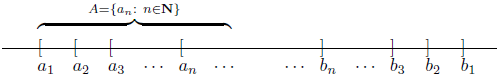
\includegraphics[width=0.8\linewidth]{figs/theorem1.4.1.png}
        \end{figure}
        Because the intervals are nested, every $b_n$ is an upper bound for $A$. So $|a_n| < b_n, \forall n \in \mathbb{N}$ and $A$ is bounded above. By the Axiom of Completeness, there exists
        \begin{equation*}
            x = \sup A.
        \end{equation*}
        
        Since $x = \sup A$, therefore $a_n \leq x, \forall n \in \mathbb{N}$. Because each $b_n$ is an upper bound for $A$, so $x \leq b_n$ since $x = \sup A$. Altogether, $a_n \leq x \leq b_n, \forall n \in \mathbb{N}$, so $x \in I_n, \forall n \in \mathbb{N}$. Hence, $x \in \bigcap_{n=1}^\infty I_n$ and $\bigcap_{n=1}^\infty I_n \neq \emptyset$.\\ \\
        QED
    
    \subsubsection{The Density of $\mathbb{Q}$ in $\mathbb{R}$}
        The set $\mathbb{Q}$ is an extension of $\mathbb{N}$, and $\mathbb{R}$ in turn is an extension of $\mathbb{Q}$. The next few results indicate how $\mathbb{N}$ and $\mathbb{Q}$ sit inside of $\mathbb{R}$.
        \\ \\
        \fbox{\parbox{\linewidth}{\textbf{Theorem 1.4.2 (Archimedean Property).}
        \begin{enumerate}[label=(\roman*)]
            \item \textit{Given any $x \in \mathbb{R}$, there exists $\exists n \in \mathbb{N}$ satisfying $n > x$.}
            \item \textit{Given any $y>0$, $y \in \mathbb{R}$, there exists $\exists n \in \mathbb{N}$ satisfying $1/n < y$.}
        \end{enumerate}}}
        \\ \\
        \textit{Proof.} (i) For contradiction, assume $\mathbb{N}$ is bounded above. By Axiom of Completeness, there exist $\alpha = \sup \mathbb{N}$. Consider $\alpha -1$, by Lemma 1.3.8,
        \begin{equation*}
            \exists n \in \mathbb{N}: \alpha - 1 < n \implies \alpha < n + 1
        \end{equation*}
        Because $n+1 \in \mathbb{N}$, $\alpha$ is not an upper bound for $\mathbb{N}$, a contradiction. Hence, $\mathbb{N}$ is not bounded above.
        \\ \\
        (ii) Let $x=1/y$, then by (i), 
        \begin{equation*}
           \forall x \in \mathbb{R}, \exists n \in \mathbb{N}: n > \frac{1}{y} \implies \frac{1}{n} < y.
        \end{equation*}
        QED
        \\ \\
        \fbox{\parbox{\linewidth}{\textbf{Theorem 1.4.3 (Density of $\mathbb{Q}$ in $\mathbb{R}$).} \textit{For every $a,b \in \mathbb{R}$ with $a < b$, there exists an $r \in \mathbb{Q}$ satisfying $a < r < b$.}}}
        \\ \\
        \textit{Proof.} Let $a,b \in \mathbb{R}$ with $a < b$. Consider a rational number $r = m/n,m \in \mathbb{Z},n\in \mathbb{N}$. Now choose $m,n$ so that 
        \begin{equation}
            a < \frac{m}{n} < b.
            \label{1.4.3(1)}
        \end{equation}
        The first step is to choose $n \in \mathbb{N}$ large enough so that consecutive increments of size $1/n$ are too close together to “step over” the interval $(a, b)$ (Figure \ref{theorem1.4.3}).
        \begin{figure}[ht!]
            \centering
            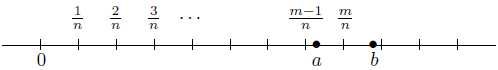
\includegraphics[width=0.8\linewidth]{figs/theorem1.4.3.png}
            \caption{}
            \label{theorem1.4.3}
        \end{figure}\\ \\
        By Archimedean Property (Theorem 1.4.2), there is $\exists n \in \mathbb{N}$ such that
        \begin{equation}
            \frac{1}{n} < b-a \implies 1 < nb - na.
            \label{1.4.3(2)}
        \end{equation}
        With $n$ already chosen, now consider an $m \in \mathbb{Z}$ to be the smallest integer greater than $na$ such that
        \begin{equation}
            m-1 \leq na
            \label{1.4.3(3)}
        \end{equation}
        and
        \begin{equation}
            na < m.
            \label{1.4.3(4)}
        \end{equation}
        By inequality (\ref{1.4.3(4)}),
        \begin{equation*}
            na < m \implies a < \frac{m}{n}.
        \end{equation*}
        By inequality (\ref{1.4.3(2)}),
        \begin{align*}
            1 < nb - na \implies na < nb -1.
        \end{align*}
        Therefore, by inequality (\ref{1.4.3(3)}),
        \begin{gather*}
            m-1 \leq na < nb-1 \implies m < nb \\
            \therefore \frac{m}{n} < b.
        \end{gather*}
        Altogether,
        \begin{equation*}
            a < \frac{m}{n} < b.
        \end{equation*}
        QED \\
        
        Theorem 1.4.3 says that $\mathbb{Q}$ is dense in $\mathbb{R}$. This result can be used to show that the irrational numbers are dense in $\mathbb{R}$ as well.
        \\ \\
        \fbox{\parbox{\linewidth}{\textbf{Corollary 1.4.4.} \textit{Given $a < b$ for $a,b \in \mathbb{R}$, there exists an irrational number $t$ such that $a < t < b$.}}}
        \\ \\
        \textit{Proof.} Let $a<b$ with $a,b \in \mathbb{R}$. Now consider $a - \sqrt{2} < b - \sqrt{2}$ with $a-\sqrt{2},b-\sqrt{b}\in \mathbb{R}$. By Theorem 1.4.3, there exists $\exists r \in \mathbb{Q}$ such that
        \begin{equation*}
            a-\sqrt{2} < r < b-\sqrt{2} \Rightarrow a < r + \sqrt{2} < b.
        \end{equation*}
        Consider an irrational number $t \in \mathbb{I}$. Assume that $r+t, rt \notin \mathbb{I}$, then
        \begin{equation*}
            t = (r+t)-r \text{ and } t = rt\bigg(\frac{1}{r}\bigg)
        \end{equation*}
        are rational numbers because $\mathbb{Q}$ is closed under addition and multiplication. But this contradicts the assumption that $t \in \mathbb{I}$. Hence, $r+t,rt \in \mathbb{I}$.\\ \\
        Therefore, $a<r+\sqrt{2}<b$ for $r + \sqrt{2} \in \mathbb{I}$.\\ \\
        QED
    
    \subsubsection{The Existence of Square Roots}
        \fbox{\parbox{\linewidth}{\textbf{Theorem 1.4.5.} \textit{There exists an $\alpha \in \mathbb{R}$ such that $\alpha^2 =2$.}}}
        \\ \\
        \textit{Proof.} Consider the set
        \begin{equation*}
            T = \{t \in \mathbb{R}: t^2 < 2\}.
        \end{equation*}
        Since $T$ is bounded above, there exists an $\alpha = \sup T$.\\ \\
        If $\alpha^2 < 2$, consider $a+(1/n) > \alpha$, so
        \begin{equation*}
            \bigg( \alpha + \frac{1}{n} \bigg)^2 = \alpha^2 + \frac{2\alpha}{n}+\frac{1}{n^2} < \alpha^2 + \frac{2\alpha}{n}+\frac{1}{n} = \alpha^2 + \frac{2\alpha+1}{n}.
        \end{equation*}
        Now choose $n_0 \in \mathbb{N}$ large enough so that
        \begin{equation*}
            \frac{1}{n_0} < \frac{2-\alpha^2}{2\alpha+1} \implies \frac{2\alpha+1}{n_0} < 2-\alpha^2.
        \end{equation*}
        Consequently,
        \begin{equation*}
            \bigg( \alpha + \frac{1}{n_0} \bigg)^2 < \alpha^2 + \frac{2\alpha+1}{n_0} < \alpha^2 + (2-\alpha^2) = 2.
        \end{equation*}
        Thus, $\alpha + (1/n_0) > \alpha$ and $\alpha + (1/n_0) \in T$, contradicting that $\alpha = \sup T$. Hence, $a^2 \nless 2$.\\ \\
        If $\alpha^2 > 2$, consider $\alpha - (1/n) < \alpha$, so
        \begin{equation*}
            \bigg(\alpha - \frac{1}{n}\bigg)^2 = \alpha^2 - \frac{2\alpha}{n} + \frac{1}{n^2} > \alpha^2 - \frac{2\alpha}{n}.
        \end{equation*}
        Now choose $n_0 \in \mathbb{N}$ larger enough so that
        \begin{equation*}
            \frac{1}{n_0} < \frac{\alpha^2 - 2}{2\alpha} \Rightarrow \frac{2\alpha}{n_0} < \alpha^2 -2.
        \end{equation*}
        So 
        \begin{equation*}
            \bigg(\alpha-\frac{1}{n_0}\bigg)^2 > \alpha^2 - \frac{2\alpha}{n_0} > \alpha^2 - (\alpha^2 -2) = 2.
        \end{equation*}
        This means $\alpha - (1/n_0)$ is an upper bound for $T$. But $\alpha - (1/n_0) < \alpha$ and this contradicts that $\alpha = \sup T$. Hence $\alpha^2 \ngtr 2$, the only possibility is $\alpha^2 = 2 \implies \alpha=\sqrt{2}$.\\ \\
        QED\\
        
        A small modification of this proof can be made to show that $\sqrt{x}$ exists for any $x \geq 0$. A formula for expanding $(\alpha + \frac{1}{n})^m$ called the binomial formula can be used to show that $\sqrt[m]{x}$ exists for arbitrary values of $m \in \mathbb{N}$.
    
    \subsection{Cardinality}
    \subsubsection{$\textbf{1-1}$ Correspondence}
        \textit{Cardinality} is the size of a set. The cardinalities of finite sets can be compared by attaching a natural number to each set.
        \\ \\
        \fbox{\parbox{\linewidth}{\textbf{Definition 1.5.1.} A function $f: A \to B$ is
        \begin{enumerate}[label=(\roman*)]
            \item \textit{One-to-one/injective} (1-1) if $a_1 \neq a_2 \implies f(a_1) \neq f(a_2)$ for $a_1,a_2 \in A$ and $f(a_1),f(a_2)\in B$.
            \item \textit{Onto/surjective} if, given any $b \in B$, it is possible to find an element $a \in A$ for which $f(a) = b$.
        \end{enumerate}}}
        \\
        
        A function $f:A \to B$ that is both 1-1 and onto (bijection) means a \textit{1-1 correspondence} between $A$ and $B$. 
        \\ \\
        \fbox{\parbox{\linewidth}{\textbf{Definition 1.5.2.} If there exists $f:A \to B$ that is 1-1 and onto, then $A$ \textit{has the same cardinality as} $B$, written $A\sim B$.}}
        \\ \\ \\
        \textbf{Example 1.5.3.} (i) Let $E = \{2,4,6,\dots\}$ be the set of even numbers and let $f:\mathbb{N} \to E$ be given by $f(n)=2n$. Then, $\mathbb{N} \sim E$ (Figure \ref{exp1.5.3(i)}).
        \begin{figure}[ht!]
            \centering
            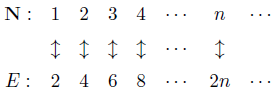
\includegraphics[width=0.4\linewidth]{figs/example1.5.3(i).png}
            \caption{}
            \label{exp1.5.3(i)}
        \end{figure}
        Certainly $E \subset \mathbb{N}$, and it seems logical that $E < \mathbb{N}$. This is one point of view that is biased to finite sets. From the point of view of the definition of cardinality, $E$ and $\mathbb{N}$ are equivalent.\\ \\
        (ii) Although $\mathbb{N} \subset \mathbb{Z}$, let
        \begin{equation*}
            f(n) = \bigg\{ \begin{matrix} (n-1)/2 & \text{if $n$ is odd} \\ -n/2 & \text{ if $n$ is even.}\end{matrix}
        \end{equation*}
        Then $\mathbb{N} \sim \mathbb{Z}$ (Figure \ref{exp1.5.3(ii)}).
        \begin{figure}[ht!]
            \centering
            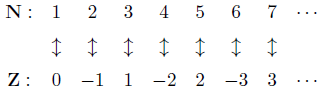
\includegraphics[width=0.45\linewidth]{figs/example1.5.3(ii).png}
            \caption{}
            \label{exp1.5.3(ii)}
        \end{figure}
        The important details are that $f$ does not map any two natural numbers to the same element of $\mathbb{Z}$ (1–1) and that every element of $\mathbb{Z}$ gets “hit” by an element in $\mathbb{N}$ (onto).\\ \\
        \textbf{Example 1.5.4.} Calculus shows that $f(x) = x/(x^2-1)$ takes the interval $(-1,1)$ onto $\mathbb{R}$ in a 1-1 fashion. Thus $(-1,1) \sim \mathbb{R}$ (Figure \ref{exp1.5.4}). In fact, $(a,b) \sim \mathbb{R}$ for any interval $(a,b)$.
        \begin{figure}[ht!]
            \centering
            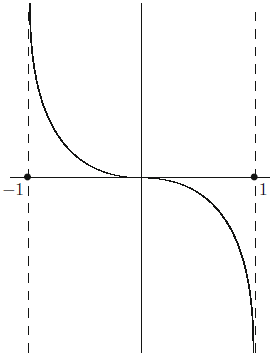
\includegraphics[width=0.35\linewidth]{figs/exp1.5.4.png}
            \caption{$(-1,1) \sim \mathbb{R}$ using $f(x) = x/(x^2-1)$.}
            \label{exp1.5.4}
        \end{figure}
        
        \subsubsection{Countable Sets}
            \fbox{\parbox{\linewidth}{\textbf{Definition 1.5.5.} A set $A$ is \textit{countable} if $\mathbb{N} \sim A$. An infinite set that is not countable is called an \textit{uncountable} set.}}
            \\ \\ \\
            \fbox{\parbox{\linewidth}{\textbf{Theorem 1.5.6.} (i) \textit{The set $\mathbb{Q}$ is countable.} (ii) \textit{The set $\mathbb{R}$ is uncountable.}}}
            \\ \\
            \textit{Proof.} (i) Set $A_1 = \{0\}$ and for each $n \geq 2$, let $A_n$ be the set given by
            \begin{equation*}
                A_n = \bigg\{\pm\frac{p}{q}:p,q \in \mathbb{N} \text{ are in lowest terms with } p+q=n\bigg\}.
            \end{equation*}
            The first few terms of the sets look like
            \begin{align*}
                A_1 & = \{0\}, \\ 
                A_2 & =\bigg\{\frac{1}{1},\frac{-1}{1}\bigg\}, \\
                A_3 & = \bigg\{\frac{1}{2},\frac{-1}{2},\frac{2}{1},\frac{-2}{1}\bigg\}, \\
                A_4 & = \bigg\{\frac{1}{3},\frac{-1}{3},\frac{3}{1},\frac{-3}{1}\bigg\}, \\
                A_5 & = \bigg\{\frac{1}{4},\frac{-1}{4},\frac{2}{3},\frac{-2}{3},\frac{3}{2},\frac{-3}{2},\frac{4}{1},\frac{-4}{1}\bigg\}.
            \end{align*}
            Each $A_n$ is \textit{finite} and every rational number appears in exactly one of these sets. The 1-1 correspondence with $\mathbb{N}$ is then achieved by consecutively listing the elements in each $A_n$.
            \begin{figure}[ht!]
                \centering
                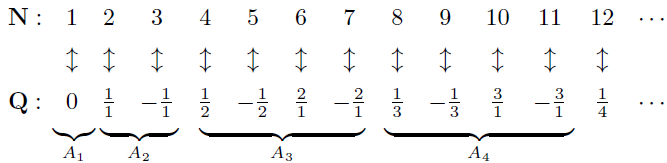
\includegraphics[width=0.8\linewidth]{figs/theorem1.5.6.png}
            \end{figure}\\
            Writing an explicit formula for this correspondence would be an awkward task and not the best use of time. What matters is that every rational number appears in the correspondence exactly once. Given, say, $22/7$, one has that $22/7 \in A_{29}$. Because the set of elements in $A_1,\dots,A_{28}$ is finite, one can be confident that $22/7$ eventually gets included in the sequence. The fact that this line of reasoning applies to any rational number $p/q$ is the proof that the correspondence is onto. To verify that it is 1–1, observe that the sets $A_n$ were constructed to be disjoint so that no rational number appears twice. This completes the proof of (i).
            \\ \\
            (ii) By contradiction, assume that there does exist a 1-1 and onto function $f:\mathbb{N} \to \mathbb{R}$. If $x_1 = f(1), x_2 = f(2), \dots$, then the assumption that $f$ is onto means that
            \begin{equation}
                \mathbb{R} = \{x_1,x_2,x_3,x_4,\dots\}
                \label{theorem1.5.6}
            \end{equation}
            and every real number appears somewhere on the list.
            
            By the Nested Interval Property, let $I_1$ be a closed interval such that $x_1 \notin I_1$. Next, let $I_2$ be a closed interval such that $I_2 \subseteq I_1$ and $x_2 \notin I_2$. In general, given an interval $I_n$, construct $I_{n+1}$ such that\\ \\
            (i) $I_{n+1} \subseteq I_n$\\ \\
            (ii) $x_{n+1} \notin I_{n+1}.$
            \begin{figure}[ht!]
                \centering
                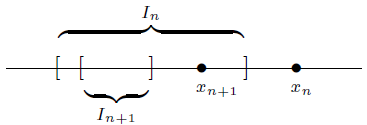
\includegraphics[width=0.5\linewidth]{figs/theorem1.5.6(2).png}
            \end{figure}\\
            Now consider the intersection $\bigcap_{n=1}^\infty I_n$. If $x_{n_0}$ is some real number from the list in (\ref{theorem1.5.6}), then $x_{n_0} \notin I_{n_0}$ and
            \begin{equation*}
                x_{n_0} \notin \bigcap_{n=1}^\infty I_n.
            \end{equation*}
            Since the assumption is that (\ref{theorem1.5.6}) contains every real number, so
            \begin{equation*}
                x_1 \notin I_1, x_2 \notin I_2, x_3 \notin I_3, \dots,
            \end{equation*}
            and
            \begin{equation*}
                \bigcap_{n=1}^\infty I_n = \emptyset.
            \end{equation*}
            But the Nested Interval Property states that $\bigcap_{n=1}^\infty I_n \neq \emptyset$. Hence, there is at least one $x \in \bigcap_{n=1}^\infty I_n$ that, consequently, cannot be on the list in (\ref{theorem1.5.6}). This contradiction means that such an enumeration of $\mathbb{R}$ is impossible, and that $\mathbb{R}$ is an \textit{uncountable} set.\\ \\
            QED \\
            
            Theorem 1.5.6 states that the cardinality of $\mathbb{R}$ is, informally speaking, a larger type of infinity. The real numbers so outnumber the natural numbers that there is no way to map $\mathbb{N}$ onto $\mathbb{R}$. The set $\mathbb{Q}$, on the other hand, is countable. As far as infinite sets are concerned, this is as small as it gets.
            \\ \\
            \fbox{\parbox{\linewidth}{\textbf{Theorem 1.5.7.} \textit{If $A \subseteq B$ and $B$ is countable, then $A$ is either countable or finite.}}}
            \\ \\
            \textit{Proof.} Assume $B$ is a countable set. Thus, there exists $f:\mathbb{N} \to B$, which is 1-1 and onto.
            
            Let $A$ be infinite for $A \subseteq B$. Define $g:\mathbb{N} \to A$, let $g(1) = f(n_1)$ for $n_1 = min\{n \in \mathbb{N}: f(n) \in A\}$. Next, let $g(2) = f(n_2)$ for $n_2 = min\{n \in \mathbb{N}: f(n) \in A \setminus \{f(n_1)\}\}$. In general, assume $g(k) = f(n_k)$ for $k<m$ is defined, and let $g(m) = f(n_m)$ for $n_m = min\{n \in \mathbb{N}: f(n) \in A \setminus \{f(n_1), \dots, f(n_{m-1}\}\}$.
            
            Since $m \neq m' \implies n_m \neq n_{m'}$ and because $f$ is assumed to be 1-1, $g(m) = f(n_m) \neq f(n_{m'}) = g(m')$, therefore $g$ is 1-1. Now let $a \in A$ be arbitrary. Because $f$ is onto, there exists $\exists n' \in \mathbb{N}$ such that $f(n')=a$. So $n' \in \{n \in \mathbb{N} : f(n) \in A\}$ and there exists $\exists n \in \mathbb{N}$ such that $g(n) = f(n') = a$ for $n'$ is the minimum of the set. Hence, $g$ is onto.
            
            Since there exists a function $g: \mathbb{N} \to A$ which is 1-1 and onto, $A$ is countable.\\ \\
            QED \\ \\
            \fbox{\parbox{\linewidth}{\textbf{Theorem 1.5.8.} (i) \textit{If $A_1, A_2,\dots,A_m$ are each countable sets, then the union $A_1 \cup A_2 \cup \dots \cup A_m$ is countable.}\\
            (ii) \textit{If $A_n$ is a countable set for each $n \in \mathbb{N}$, then $\bigcup_{n=1}^\infty A_n$ is countable.}}}
            \\ \\
            \textit{Proof.} (i) Let $A_1$ and $A_2$ be two countable sets. First, replace $A_2$ with the set $B_2 = A_2 \setminus A_1 = \{x \in A_2 : x \notin A_1\}$. So that $A_1 \cup B_2 = A_1 \cup A_2$ and $A_1 \cap B_2 = \emptyset$.
            
            Because $A_1$ is countable, there exists a 1-1 and onto function $f: \mathbb{N} \to A_1$. If $B_2 = \emptyset$, then $A_1 \cup A_2 = A_1$ which is countable. If $B_2 = \{b_1,b_2,\dots,b_m\}$, then define $h:\mathbb{N} \to A_1 \cup B_2$ via
            \begin{equation*}
                h(n) = \bigg\{ \begin{matrix} b_n & \text{if } n \leq m \\ f(n-m) & \text{ if } n > m.\end{matrix}
            \end{equation*}
            The fact that $h$ is 1-1 and onto follows immediately from the same properties of $f$.
            
            If $B_2$ is infinite, then by Theorem 1.5.7 it is countable, and so there exists a 1-1 and onto function $g: \mathbb{N} \to B_2$. In this case define $h: \mathbb{N} \to A_1 \cup B_2$ by
            \begin{equation*}
                h_n = \bigg\{ \begin{matrix} f\big(\frac{n+1}{2}\big) & \text{if $n$ is odd} \\
                g\big(\frac{n}{2}\big) & \text{ if $n$ is even.}\end{matrix}
            \end{equation*}
            Again, the proof that $h$ is 1-1 and onto is derived directly from the fact that $f$ and $g$ are both bijections. Graphically, the correspondence takes the form of Figure (\ref{theorem1.5.8}).
            \begin{figure}[ht!]
                \centering
                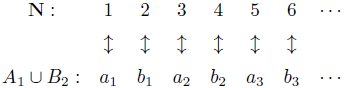
\includegraphics[width=0.5\linewidth]{figs/theorem1.5.8.png}
                \caption{}
                \label{theorem1.5.8}
            \end{figure}
            
            Now assume that the union of $m$ countable sets is countable, given $m+1$ countable sets $A_1,A_2,\dots,A_{m+1}$, one can write
            \begin{equation*}
                A_1 \cup A_2 \cup \dots \cup A_{m+1} = (A_1 \cup A_2 \cup \dots \cup A_m) \cup A_{m+1}.
            \end{equation*}
            Then $C_m = A_1 \cup \dots \cup A_m$ is countable by the induction hypothesis, and $C_m \cup A_{n+1}$ is just the union of two countable sets which is countable. This completes the proof.\\ \\
            (ii) First consider the case where the sets $\{A_n\}$ are disjoint. To achieve 1-1 correspondence between the set $\mathbb{N}$ and $\bigcup_{n=1}^\infty A_n$, first label the elements in each countable set $A_n$ as
            \begin{equation*}
                A_n = \{a_{n1},a_{n2},a_{n3},\dots\}.
            \end{equation*}
            Now arrange the elements of $\bigcup_{n=1}^\infty A_n$ in an array similar to the one for $\mathbb{N}$ shown by Figure (\ref{theorem1.5.8(1)}) like Figure (\ref{theorem1.5.8(2)}).
            \begin{figure}[ht!]
                \centering
                \begin{subfigure}[b]{0.35\linewidth}
                    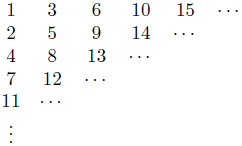
\includegraphics[width=\linewidth]{figs/theorem1.5.8(1).png}
                    \caption{}
                    \label{theorem1.5.8(1)}
                \end{subfigure}
                \begin{subfigure}[b]{0.45\linewidth}
                    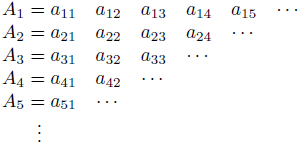
\includegraphics[width=\linewidth]{figs/theorem1.5.8(2).png}
                    \caption{}
                    \label{theorem1.5.8(2)}
                \end{subfigure}
            \caption{}
            \end{figure}
            This establishes a 1-1 and onto mapping $g: \mathbb{N} \to \bigcup_{n=1}^\infty A_n$ where $g(n)$ corresponds to the element $a_{jk}$ where $(j,k)$ is the row and column location of $n$ in the array for $\mathbb{N}$. Hence $\bigcup_{n=1}^\infty A_n$ is countable.
            
            If the sets $\{A_n\}$ are not disjoint then the mapping may not be 1-1. In this case one could again replace $A_n$ with $B_n = A_n \setminus \{A_1 \cup \dots \cup A_{n-1}\}$. Another approach is to use the previous argument to establish a 1-1 correspondence between $\bigcup_{n=1}^\infty A_n$ and an infinite subset of $\mathbb{N}$, and then appeal to Theorem 1.5.7.\\ \\
            QED\\
            
            Because $\mathbb{R} = \mathbb{Q} \cup \mathbb{I}$ and $\mathbb{R}$ is not countable, it follows that $\mathbb{I}$ cannot be countable because otherwise $\mathbb{R}$ would be. Hence the irrational numbers form a far greater subset of $\mathbb{R}$ than $\mathbb{Q}$.
            
            A real number $x \in \mathbb{R}$ is called \textit{algebraic} if there exist $a_0,a_1,a_2,\dots,a_n \in \mathbb{Z}$, not all zero, such that
            \begin{equation*}
                a_nx^n + a_{n-1}x^{n-1}+\dots+a_1x+a_0 = 0.
            \end{equation*}
            Said another way, a real number is algebraic if it is the root of a polynomial with integer coefficients. Real numbers that are not algebraic are called \textit{transcendental numbers}.\\ \\
            \textbf{Example:} $x = \sqrt{2}$ is the root of the polynomial $x^2-2=0$. $x = \sqrt[3]{2}$ is the root of the polynomial $x^3-2=0$. $x=\sqrt{3}+\sqrt{2}$ is the root of the polynomial $x^4-10x^2+1=0$. Hence, $\sqrt{2},\sqrt[3]{2}$, and $\sqrt{3}+\sqrt{2}$ are all algebraic.\\ \\
            \fbox{\parbox{\linewidth}{\textbf{Theorem 1.5.9. (Schr$\mathbf{\Ddot{o}}$der-Bernstein Theorem)} If there exists a 1-1 function $f:X \to Y$ and another 1-1 function $g: Y \to X$. Then there exists a 1-1,onto function $h: X \to Y$ and hence $X \sim Y$.}}
            
        
        \subsection{Cantor's Theorem}
        \subsubsection{Cantor's Diagonalization Method}
            \fbox{\parbox{\linewidth}{\textbf{Theorem 1.6.1.} \textit{The open interval $(0,1)=\{x \in \mathbb{R}: 0<x<1\}$ is uncountable.}}}
            \\ \\
            \textit{Proof.} By contradiction, assume that there exists a 1-1 and onto function $f: \mathbb{N} \to (0,1)$. For $\forall m \in \mathbb{N}$, one has $0 < f(m) \in \mathbb{R} < 1$. Representing $f(m)$ using decimal notation
            \begin{equation*}
                f(m) = .a_{m1}a_{m2}a_{m3}a_{m4}a_{m5}\dots.
            \end{equation*}
            For $m,n \in \mathbb{N}$, $a_{m,n} \in \{0,1,2,\dots,9\}$ represents the $n$th digit in the decimal expansion of $f(m)$. The 1-1 correspondence between $\mathbb{N}$ and $(0,1)$ can be summarized in the doubly indexed array (Figure \ref{theorem1.6.1}).
            \begin{figure}[ht!]
                \centering
                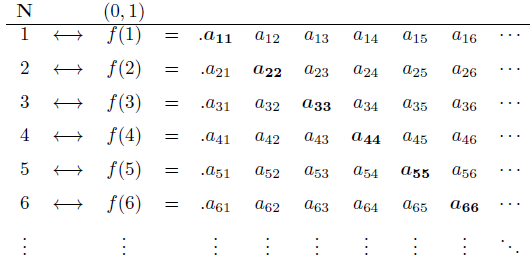
\includegraphics[width=0.8\linewidth]{figs/theorem1.6.1.png}
                \caption{}
                \label{theorem1.6.1}
            \end{figure}
            The key assumption about this correspondence is that $\forall x \in (0,1), x \in \mathbb{R}$ is assumed to appear somewhere on the list.
            
            Now, define $x \in (0,1), x \in \mathbb{R}$ with the decimal expansion $x=.b_1 b_2 b_3 b_4 \dots$ using the rule
            \begin{equation*}
                b_n = \bigg\{ \begin{matrix} 2 & \text{if } a_{nn} \neq 2 \\ 3 & \text{ if } a_{nn} = 2. \end{matrix}
            \end{equation*}
            To compute $b_1$, look at $a_{11}$ in the upper left-hand coner of the array. If $a_{11}=2$, then $b_1=3$; otherwise, $b_1=2$.
            
            Then, the real number $x=.b_1b_2b_3\dots \neq f(1)=.a_{11}a_{22}a_{33}\dots$ because $b_1 \neq a_{11}$ (since $b_1 = 2$ if $a_{11} \neq 2$, and $b_1 = 3$ if $a_{11} = 2$). Further, $x \neq f(2)=.a_{21}a_{22}a_{23}\dots$ because $b_2 \neq a_{22}$. In general, $x \neq f(n)$ because $b_n \neq a_{nn}$.
            
            Since $f$ is onto, $\forall x\in (0,1),x\in \mathbb{R}$ should be in the indexed array $\{f(1), f(2), f(3), \dots\}$. However, $x \neq f(n)$ for $\forall n \in N$, and hence is not contained in the range of $f$. This is a contradiction to the assumption that $f$ is onto. Hence, $(0,1)$ is uncountable.\\ \\
            QED \\ \\
            \textbf{Example:} Let $S$ be the set consisting of all sequences of 0's and 1's
            \begin{equation*}
                S = \{(a_1,a_2,a_3,\dots):a_n = 0 \text{ or } 1\}.
            \end{equation*}
            For example, $(1,0,1,0,\dots) \in S$ and $(1,1,1,1,\dots) \in S$.
            
            Assume that $S$ is countable and hence there exists a 1-1 and onto function $f: \mathbb{N} \to S$. The 1-1 correspondence between $\mathbb{N}$ and $S$ can be represented by Figure \ref{theorem1.6.1} where $a_{m,n} = 1 \text{ or } 0$ for $m,n \in \mathbb{N}$. Now define a sequence $(x_n) = (x_1,x_2,x_3,\dots) \in S$ via
            \begin{equation*}
                x_n = \bigg\{ \begin{matrix}0 & \text{if } a_{nn} = 1 \\ 1 & \text{ if } a_{nn} = 0.\end{matrix}
            \end{equation*}
            
            From this definition, $(x_n) \neq f(1)$ because $x_1 \neq a_{11}$, $(x_n) \neq f(2)$ because $x_2 \neq a_{22}$, and in general $(x_n) \neq f(n)$ because $x_n \neq a_{nn}$ for $\forall x \in \mathbb{N}$. Since $f$ is onto, all sequences in $S$ should be in the range of $f$. However, the particularly defined $(x_n) \neq f(n)$ for $\forall n \in \mathbb{N}$. This contradicts the assumption that $f$ is onto and thus $S$ is uncountable. 
        
        \subsubsection{Power Sets and Contor's Theorem}
            Given a set $A$, the \textit{power set} $P(A)$ of $A$ is the collection of all subsets of $A$. $P(A)$ itself is a set whose elements are the different possible subsets of $A$. For example, for the set $A = \{a,b,c\}$, its power set is
            \begin{equation*}
                P(A) = \{\emptyset,\{a\},\{b\},\{c\},\{a,b\},\{a,c\},\{b,c\},\{a,b,c\}\}.
            \end{equation*}
            \\
            \fbox{\parbox{\linewidth}{\textbf{Theorem 1.5.2. (Cantor's Theorem).} \textit{Given any set $A$, there does not exist a function $f: A \to P(A)$ that is onto.}}}
            \\ \\
            \textit{Proof.} For contradiction, assume that $f:A \to P(A)$ is onto. Then, construct $B$ using the following rule. For each element $a \in A$, consider the subset $f(a)$ which may contain the element $a$ or not. If $f(a)$ does not contain $a$, then $a$ is included in $B$. So
            \begin{equation*}
                B = \{a \in A: a \notin f(a)\}.
            \end{equation*}
            For example, if $A = \{1,2,3\}$, and 
            \begin{align*}
                f(1) & = \{1\}\\
                f(2) & = \{1,3\}\\
                f(3) & = \{1,2,3\},
            \end{align*}
             then $B=\{2\}$. If 
             \begin{align*}
                f(1) & = \{2,3\}\\
                f(2) & = \emptyset\\
                f(3) & = \{1,3\},
            \end{align*}
            then $B=\{1,2\}$.
            So $B \in P(A)$. Since $f$ is onto, there must exists $\exists a' \in A$ such that $B = f(a')$.
            
            If $a' \in B$, then by the definition of $B$, $a' \notin f(a')$. But $B = f(a')$ which means that $a' \notin B$, a contradiction. Hence $a' \in B$ is false. If $a' \notin B$, then by the definition of $B$, $a' \in f(a')$. Because $B = f(a')$, this implies that $a' \in B$, a contradiction. Therefore $a' \notin B$ is also false.
            
            Since it is impossible for $a'$ to be in neither $B$ nor $B^c$, the assumption that $B=f(a')$ for $\exists a' \in A$ must be false. So such an element $a'$ does not exist, and $f$ is not onto.\\ \\
            QED\\ \\
        
        \section{Sequence and Series}
        \subsection{Discussion: Rearrangements of Infinite Series}
            Consider the infinite series
            \begin{equation*}
                \sum_{n=1}^\infty \frac{(-1)^{n+1}}{n} = 1 - \frac{1}{2} + \frac{1}{3} - \frac{1}{4} + \frac{1}{5} - \frac{1}{6} + \frac{1}{7} - \frac{1}{8} + \dots.    
            \end{equation*}
            Adding from left-hand side gives a sequence $(s_n)$ called \textit{partial sum}. Let $s_n$ be the sum of the first $n$ terms, then $s_1 = 1,s_2=1/2,s_3=5/6,s_4=7/12,\dots$. It can be seen that the successive sums oscillate in a progressively narrower space. The odd sums decrease ($s_1>s_3>s_5>\dots$) while the even sums increase ($s_2<s_4<s_6<\dots$).
            
            It seems reasonable that the sequence $(s_n)$ eventually hones in on a value, call it $S$, where the odd and even partial sums "meet". $S$ cannot be computed precisely for now, but it falls somewhere between $7/12$ and $5/6$. Summing a few hundred terms reveals that $S\approx0.69$.
            \begin{figure}[ht!]
                \centering
                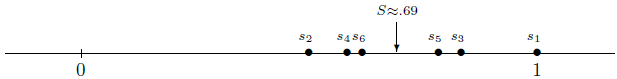
\includegraphics[width=0.9\linewidth]{figs/2.1.png}
            \end{figure}
            
            There is now an temptation to write
            \begin{equation}
                S = 1 - \frac{1}{2} + \frac{1}{3} - \frac{1}{4} + \frac{1}{5} - \frac{1}{6} + \frac{1}{7} - \frac{1}{8} + \dots,
            \label{infinite sum}
            \end{equation}
            meaning if all infinitely many of these numbers can be added up, then the sum would equal $S$. A more familiar example would be
            \begin{equation*}
                2 = 1 + \frac{1}{2} + \frac{1}{4} + \frac{1}{8} + \frac{1}{16} + \frac{1}{32} + \frac{1}{64} + \dots,
            \end{equation*}
            the only difference is that the second equation has a more recognizable value for the sum.
            
            Treating equation (\ref{infinite sum}) in a standard algebraic way, multiply it by 1/2 and add it back to equation (\ref{infinite sum}):
            \begin{align*}
                    \frac{1}{2}S & = \qquad \frac{1}{2} \qquad - \frac{1}{4} \qquad + \frac{1}{6} \qquad - \frac{1}{8} \qquad + \frac{1}{10} \qquad - \frac{1}{12} \qquad + \dots\\
                +S & = 1   -\frac{1}{2} +\frac{1}{3} -\frac{1}{4} +\frac{1}{5} -\frac{1}{6} +\frac{1}{7} -\frac{1}{8} +\frac{1}{9} -\frac{1}{10} +\frac{1}{11} -\frac{1}{12} +\frac{1}{13} -\dots
            \end{align*}
            \hrule
            \begin{equation}
                \frac{3}{2}S = 1 \qquad +\frac{1}{3} - \frac{1}{2} + \frac{1}{5} \qquad + \frac{1}{7} - \frac{1}{4} + \frac{1}{9} \qquad + \frac{1}{11} - \frac{1}{6} + \frac{1}{13} + \dots.
            \label{infinite sum 2}
            \end{equation}
            The sum in equation (\ref{infinite sum 2}) consists precisely of the same terms as those in equation (\ref{infinite sum}), only in different order. Specifically, the series in equation (\ref{infinite sum 2}) is a rearrangement of equation (\ref{infinite sum}) where the first two positive terms ($1+\frac{1}{3}$) are followed by the first negative term ($-\frac{1}{2}$), followed by the next two positive terms ($\frac{1}{5}+\frac{1}{7}$) and then the next negative term ($-\frac{1}{4}$). But equation (\ref{infinite sum 2}) states that the sum of these rearranged, but unaltered, numbers is equal to 3/2 of its original value. Indeed, adding a few hundred terms of equation (\ref{infinite sum 2}) produces partial sums in the neighborhood of 1.03. Infinite addition is not commutative.
            
            Consider another series
            \begin{equation*}
                \sum_{n=1}^\infty (-\frac{1}{2})^n.
            \end{equation*}
            This series is geometric with first term 1 and common ratio $r=-1/2$. Using the formula $1/(1-r)$ for the sum of a geometric series,
            \begin{equation*}
                1-\frac{1}{2}+\frac{1}{4}-\frac{1}{8}+\frac{1}{16}-\frac{1}{32}+\frac{1}{64}-\frac{1}{128}+\frac{1}{256}-\dots = \frac{1}{1-(-\frac{1}{2})} = \frac{2}{3}.
            \end{equation*}
            The "two positives, one negative" rearrangement
            \begin{equation*}
                1+\frac{1}{4}-\frac{1}{2}+\frac{1}{16}+\frac{1}{64}-\frac{1}{8}+\frac{1}{256}+\frac{1}{1024}-\frac{1}{32}+\dots
            \end{equation*}
            produces partial sum quite close to 2/3. Infinite addition is commutative in some instances but not in others.

        \subsection{The Limit of a Sequence}
            \fbox{\parbox{\linewidth}{\textbf{Definition 2.2.1.} A \textit{sequence} is a function whose domain is $\mathbb{N}$.}}
            \\ \\
            Definition 2.2.1 depicts a sequence as an ordered list of real numbers. Given a function $f: \mathbb{N} \to \mathbb{R}$, $f(n)$ is the $n$th term on the list.\\ \\
            \textbf{Example 2.2.2.} The following are common ways to describe a sequence.
            (i) $\big(1,\frac{1}{2},\frac{1}{3},\frac{1}{4},\dots\big)$\\ \\
            (ii) $\big(\frac{1+n}{n}\big)_{n=1}^\infty = \big(\frac{2}{1},\frac{3}{2},\frac{4}{3},\dots\big)$\\ \\
            (iii) $(a_n)=(2,4,8,16,\dots)$, where $a_n=2^n$ for each $n \in \mathbb{N}$\\ \\
            (iv) $(x_n)=\big(2,\frac{3}{2},\frac{5}{4},\dots\big)$, where $x_1=2$ and $x_{n+1} = \frac{x_n+1}{2}$
            \\ \\
            \fbox{\parbox{\linewidth}{\textbf{Definition 2.2.3 (Convergence of a Sequence).} A sequence $(a_n)$ \textit{converges} to $a \in \mathbb{R}$ if, for $\forall \epsilon > 0$, there exists $\exists N \in \mathbb{N}$ such that whenever $n \geq N$ it follows that $|a_n - a| < \epsilon$. If $(a_n)$ converges to $a$, then $\lim a_n = a$ or $(a_n) \to a$.}}
            \\ \\
            \fbox{\parbox{\linewidth}{\textbf{Definition 2.2.4.} Given $a \in \mathbb{R}$ and $\epsilon > 0$, the set
            \begin{equation*}
                V_\epsilon(a) = \{x \in \mathbb{R} : |x-a| < \epsilon\}
            \end{equation*}
            is called the \textit{$\epsilon$-neighborhood of $a$}.}}
            \\ \\
            
            $V_\epsilon(a)$ consists of all the points whose distance from $a$ is less than $\epsilon$,
            \begin{gather*}
                |x-a|<\epsilon \implies -(x-a)<\epsilon \implies x-a>-\epsilon \quad \text{and} \quad x-a < \epsilon\\
                \therefore -\epsilon < x-a < \epsilon \implies a-\epsilon < x < a+\epsilon.
            \end{gather*}
            So $V_\epsilon(a)$ is an interval, centered at $a$ with radius $\epsilon$.
            \begin{figure}[ht!]
                \centering
                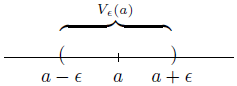
\includegraphics[width=0.35\linewidth]{figs/definition2.2.4.png}
                \caption{Illustration of Definition 2.2.4.}
            \end{figure}
            \\ \\
            \fbox{\parbox{\linewidth}{\textbf{Definition 2.2.3B (Convergence of a Sequence: Topological Version).} A sequence $(a_n)$ converges to $a$ if, given any $V_\epsilon(a)$, there exists a point in the sequence after which all of the terms are in $V_\epsilon(a)$. In other words, every $V_\epsilon(a)$ contains all but a finite number of the terms of $(a_n)$.}}
            
            \begin{figure}[ht!]
                \centering
                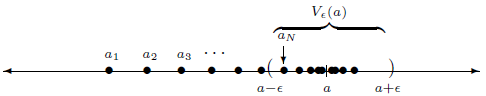
\includegraphics[width=0.8\linewidth]{figs/definition2.2.3b.png}
                \caption{Illustration of Definition 2.2.3B.}
            \end{figure}
            
            Definition 2.2.3 and Definition 2.2.3B say the same thing; $N \in \mathbb{N}$ in Definition 2.2.3 is the point where the sequence $(a_n)$ enters $V_\epsilon(a)$, never to leave. \textit{The value of $N$ depends on the choice of $\epsilon$}. The smaller the $\epsilon$-neighborhood, the larger $N$ may have to be.\\ \\
            \textbf{Example 2.2.5.} Consider the sequence $(a_n)=\big(1,\frac{1}{\sqrt{2}},\frac{1}{\sqrt{3}},\dots\big)$, where $a_n=1/\sqrt{n}$. Intuitively,
            \begin{equation*}
                \lim \bigg(\frac{1}{\sqrt{n}}\bigg) = 0.
            \end{equation*}
            Let $\epsilon=1/10$, so $V_\epsilon(0)=(-1/10,1/10)$ centered around the limit 0. The 100th term $a_{100} = 1/\sqrt{100}=1/10$ is right on the boundary, so
            \begin{equation*}
                \text{if} \quad n>100, \quad \text{then} \quad a_n \in \bigg(-\frac{1}{10},\frac{1}{10}\bigg).
            \end{equation*}
            Thus, for $\epsilon=1/10$, $N=101$ (or anything larger) can be chosen such that
            \begin{equation*}
                a_n \in \bigg(-\frac{1}{10},\frac{1}{10}\bigg), \quad \forall n \geq N = 101.
            \end{equation*}
            Now let $\epsilon=1/50$, $V_\epsilon(0)$ now shrinks to $(-1/50,1/50)$, and one must travel farther out into the sequence before $a_n$ falls into this interval. It requires that
            \begin{equation*}
                    a_n = \frac{1}{\sqrt{n}} < \frac{1}{50} \implies n>50^2=2500.
                \end{equation*}
                So $a_{2500} = 1/\sqrt{2500} = 1/50$ is right on the boundary. Thus, $N=2501$ is a suitable response to $\epsilon=1/50$ such that
                \begin{equation*}
                    a_n \in \bigg(-\frac{1}{50},\frac{1}{50}\bigg), \quad \forall n \geq N = 2501.
                \end{equation*}
                In general, whatever $\epsilon>0$ happens to be, it is required that
                \begin{equation*}
                    a_n = \frac{1}{\sqrt{n}}<\epsilon \implies n>\frac{1}{\epsilon^2}.
                \end{equation*}
                \textit{Proof.} Let $\epsilon>0$ be arbitrary. Choose $N \in \mathbb{N}$ such that
                \begin{equation*}
                    N>\frac{1}{\epsilon^2}.
                \end{equation*}
                Let $n\geq N$, then
                \begin{equation*}
                    n \geq N >\frac{1}{\epsilon^2} \implies \frac{1}{\sqrt{n}}<\epsilon \quad \text{and hence} \quad \bigg|\frac{1}{\sqrt{n}}-0\bigg|=|a_n-0|<\epsilon.
                \end{equation*}
                QED
            
            \subsubsection{Quantifiers}
                Template for a proof that $\lim(x_n) = x$:
                \begin{itemize}
                    \item Let $\epsilon>0$ be arbitrary.
                    \item Demonstrate a choice for $N\in \mathbb{N}$. This step usually requires the most work, almost all of which is done prior to actually writing the formal proof.
                    \item Now, show that $N$ actually works.
                    \item Assume $n\geq N$.
                    \item With $N$ chosen, it should be possible to derive the inequality $|x_n-x|<\epsilon$.
                \end{itemize}
                \textbf{Example 2.2.6.} Show
                \begin{equation*}
                    \lim \bigg(\frac{n+1}{n}\bigg)=1.
                \end{equation*}
                The last line of the proof should be that for suitably large values of $n$,
                \begin{equation*}
                    \bigg| \frac{n+1}{n}-1 \bigg| < \epsilon.
                \end{equation*}
                Since
                \begin{equation*}
                    \bigg| \frac{n+1}{n} - 1\bigg| = \frac{1}{n} \implies \frac{1}{n} < \epsilon \quad \text{or} \quad n > \frac{1}{\epsilon},
                \end{equation*}
                choosing $N > 1/ \epsilon$ will suffice.\\ \\
                \textit{Proof.} Let $\epsilon>0$ be arbitrary. Choose $N \in \mathbb{N}$ with $N>1/\epsilon$. Let $n\in \mathbb{N}$ for $n \geq N$. Then, $n \geq N > 1/\epsilon \implies n > 1/\epsilon$ and thus $1/n < \epsilon$. Hence,
                \begin{equation*}
                    \frac{1}{n}=\bigg|\frac{1}{n}\bigg|=\bigg|\frac{1}{n}+1-1\bigg|=\bigg|\frac{n+1}{n}-1\bigg| < \epsilon,
                \end{equation*}
                and $\lim((n+1)/n)=1$.\\ \\
                QED
            
            \subsubsection{Divergence}
                \textbf{Example 2.2.7.} Consider the sequence \begin{equation*}
                    \bigg(1,-\frac{1}{2},\frac{1}{3},-\frac{1}{4},\frac{1}{5},-\frac{1}{5},\frac{1}{5},-\frac{1}{5},\frac{1}{5},-\frac{1}{5},\frac{1}{5},-\frac{1}{5},\frac{1}{5},-\frac{1}{5},\dots\bigg).
                \end{equation*}
                Looking at the first few terms, it seems that this sequence converges to zero. Let $\epsilon=1/2$, it can be seen that starting from $N=3$ all the terms fall into $V_\epsilon(0)=(0-1/2,0+1/2)=(-1/2,1/2)$. But the definition of convergence says $\forall \epsilon>0$. Let $\epsilon=1/10$, there does not exist an $N$ for which the terms after which fall into $V_\epsilon(0)=(-1/10,1/10)$. Hence, the sequence does not converge to 0.
                
                Now assume that the sequence does converge to 1/5. Choosing $\epsilon=1/10$ produces $V_\epsilon(1/5)=(1/5-1/10,1/5+1/10)=(1/10,3/10)$. Although the sequence continually revisits this neighborhood, there is no point at which it enters and never leaves ($1/5 \in V_\epsilon(1/5)$ and $-1/5 \notin V_\epsilon(1/5)$). Thus, no $N$ exists for $\epsilon=1/10$, so the sequence does not converge to 1/5. Furthermore, the sequence does not converge to any other real number, so the sequence does not converge.
                \\ \\
                \fbox{\parbox{\linewidth}{\textbf{Definition 2.2.8.} A sequence that does not converge is said to \textit{diverge}.}}
            
            \subsection{The Algebraic and Order Limit Theorems}
                \fbox{\parbox{\linewidth}{\textbf{Definition 2.3.1.} A sequence $(x_n)$ is \textit{bounded} if there exists $\exists M>0$ such that $|x_n| \leq M$ for $\forall n \in \mathbb{N}$.}}
                \\ \\
                
                Geometrically, $(x_n)$ is bounded if $x_n \in [-M,M]$ for $\forall n \in \mathbb{N}$.
                \\ \\
                \fbox{\parbox{\linewidth}{\textbf{Theorem 2.3.2.} \textit{Every convergent sequence is bounded.}}}
                \\ \\
                \textit{Proof.} If a convergent sequence $(x_n)$ is bounded, then there exists $\exists M>0$ such that $|x_n| \leq M, \quad \forall n \in \mathbb{N}$.
                
                Assume $\lim x_n=l$. So given, for example, $\epsilon=1$, there exists $\exists N \in \mathbb{N}$ such that $|x_n-l|<1$ for $\forall n \geq N$. By Reverse Triangle Inequality, $|a-b| \geq |a|-|b|$, hence 
                \begin{equation*}
                    1 > |x_n-l| \geq |x_n|-|l| \implies |x_n|<|l|+1, \quad \forall n \geq N.
                \end{equation*}
                Consider the finite number of terms in the sequence that come before the $N$th term, $\{|x_1|,|x_2|,\dots,|x_{N-1}|,|l|+1\}$. Let
                \begin{equation*}
                    M=\max\{|x_1|,|x_2|,\dots,|x_{N-1}|,|l|+1\}.
                \end{equation*}
                So $M \geq |l|+1 > |x_n|,\forall n < N$, and $M \geq |l|+1 > |x_n|,\forall n \geq N$. Hence, $M \geq |a_n|, \forall n \in \mathbb{N}$. \\ \\
                QED
                \begin{figure}[ht!]
                    \centering
                    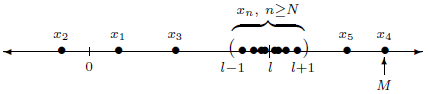
\includegraphics[width=0.6\linewidth]{figs/theorem2.3.2.png}
                    \caption{Illustration of Theorem 2.3.2.}
                \end{figure}
                \\ \\
                \fbox{\parbox{\linewidth}{\textbf{Theorem 2.3.3 (Algebraic Limit Theorem).} \textit{Let $\lim (a_n)=a$, and $\lim (b_n)=b$. Then,}
                \begin{enumerate}[label=(\roman*)]
                    \item $\lim (ca_n) = ca, \forall c \in \mathbb{R}$
                    \item $\lim (a_n+b_n) = a+b$
                    \item $\lim(a_nb_n) = ab$
                    \item $\lim(a_n/b_n) = a/b, \quad b \neq 0$
                \end{enumerate}}}
                \\ \\
                \textit{Proof.} Suppose $\lim(a_n)=a$ and $\lim(b_n)=b$.\\ \\
                (i) Assume that $\lim(ca_n)=ca$. If $c \neq 0$, let $\epsilon<0$ be arbitrary. Now,
                \begin{equation*}
                    |ca_n - ca| = |c| |a_n - a|.
                \end{equation*}
                Since $\lim(a_n)=a$, $|a_n-a|<$ anything. In particular, $N$ can be chosen such that
                \begin{equation*}
                    |a_n-a| < \frac{\epsilon}{|c|}, \quad \forall n \geq N.
                \end{equation*}
                Therefore,
                \begin{equation*}
                    |ca_n-ca| = |c| |a_n-a| < |c| \bigg(\frac{\epsilon}{|c|}\bigg) = \epsilon, \quad \forall n \geq N.
                \end{equation*}
                Hence, $|ca_n-ca|<\epsilon$ and $\lim (ca_n)=ca$.
                
                If $c=0$, then 
                \begin{equation*}
                    |ca_n-ca|=|c||a_n-a|=0.
                \end{equation*}
                Hence, for $\forall \epsilon > 0$, 
                \begin{equation*}
                    |ca_n-ca|<\epsilon,
                \end{equation*}
                for all $n \in \mathbb{N}$. So $N$ can be chosen as anything. Thus, $\lim(ca_n)=ca$.
                \\ \\
                (ii) Assume that $\lim(a_n+b_n)=a+b$. By the triangle inequality,
                \begin{equation*}
                    |(a_n + b_n) - (a+b)| = |(a_n-a)+(b_n-b)| \leq |a_n-a| + |b_n-b|.
                \end{equation*}
                Since $\lim(a_n)=a$, there exists $\exists N_1 \in \mathbb{N}$ such that
                \begin{equation*}
                    |a_n-a| < \frac{\epsilon}{2}, \quad \forall n \geq N_1. 
                \end{equation*}
                Since $\lim(b_n)=b$, there exists $\exists N_2 \in \mathbb{N}$ such that
                \begin{equation*}
                    |b_n-b| < \frac{\epsilon}{2}, \quad \forall n \geq N_2. 
                \end{equation*}
                Let $N = \max \{N_1,N_2\}$, so $n \geq N \implies n \geq N_1, n \geq N_2$. Then,
                \begin{equation*}
                    |(a_n+b_n)-(a+b)| \leq |a_n-a|+|b_n-b|<\frac{\epsilon}{2}+\frac{\epsilon}{2}=\epsilon,
                \end{equation*}
                for $\forall n \geq N$. Hence, $\lim (a_n+b_n)=a+b$.
                \\ \\
                (iii) Assume that $\lim(a_nb_n)=ab$. By triangle inequality,
                \begin{align*}
                    |a_nb_n-ab| & = |a_nb_n - ab_n + ab_n - ab|\\ & \leq |a_nb_n - ab_n| + |ab_n - ab| \\
                    & = |b_n||a_n-a|+|a||b_n-b|.
                \end{align*}
                Let $\epsilon > 0$ be arbitrary. If $a \neq 0$, since $\lim (b_n)=b$, there exists $\exists N_1 \in \mathbb{N}$ such that
                \begin{equation*}
                    |b_n - b| < \frac{1}{|a|} \frac{\epsilon}{2}, \quad \forall n \geq N_1.
                \end{equation*}
                
                By Theorem 2.3.2, every convergent sequence is bounded. Since $(b_n)$ is bounded, there exists $\exists M>0: |b_n| \leq M, \quad \forall n \in \mathbb{N}$. Now, since $\lim (a_n)=a$, there exists $\exists N_2 \in \mathbb{N}$ such that
                \begin{equation*}
                    |a_n - a| < \frac{1}{M} \frac{\epsilon}{2}, \quad \forall n \geq N_2.
                \end{equation*}
                Let $N = \max\{N_1,N_2\}$ so that $n \geq N \implies n \geq N_1, n \geq N_2$. Then, 
                \begin{align*}
                    |a_nb_n-ab| & \leq |b_n||a_n-a|+|a||b_n-b| \\
                    & \leq M|a_n-a| + |a||b_n-b| \\
                    & < M\bigg(\frac{1}{M}\frac{\epsilon}{2}\bigg) + |a|\bigg(\frac{1}{|a|}\frac{\epsilon}{2}\bigg)\\
                    & = \frac{\epsilon}{2} + \frac{\epsilon}{2}\\
                    & = \epsilon,
                \end{align*}
                for $\forall n \geq N$. Hence, $\lim (a_nb_n)=ab$.
                
                If $a=0$, then $\lim(a_n)=0$. Since $(b_n)$ is convergent, it is bounded and $|b_n| \leq M$. Consider
                \begin{equation*}
                    |a_n||b_n| = |a_nb_n| \leq |a_n|M.
                \end{equation*}
                Since $\lim (a_n)=0$, there exists $\exists N \in \mathbb{N}$ such that for $\forall \epsilon > 0$,
                \begin{equation*}
                    |a_n| < \frac{\epsilon}{M}, \quad \forall n \geq N.
                \end{equation*}
                Therefore,
                \begin{equation*}
                    |a_nb_n| \leq |a_n|M < (\frac{\epsilon}{M})M = \epsilon.
                \end{equation*}
                This implies that $|a_nb_n-0|<\epsilon$ and hence $\lim(a_nb_n)=0=ab$.
                \\ \\
                (iv) Since $\lim(a_n/b_n)=\lim(a_n(1/b_n)$=a(1/b), first prove that $\lim(1/b_n)=1/b$. Observe that
                \begin{equation*}
                    \bigg| \frac{1}{b_n} - \frac{1}{b} \bigg| = \bigg| \frac{b-b_n}{b_nb} \bigg| = \frac{|b-b_n|}{|b_n||b|}, \quad \forall b \neq 0.
                \end{equation*}
                Let $\epsilon_0=|b|/2$. Since $\lim (b_n)=b$, there exists $\exists N_1 \in \mathbb{N}$ such that
                \begin{equation*}
                    |b_n - b| < \frac{|b|}{2}, \quad \forall n \geq N_1.
                \end{equation*}
                This implies $|b_n| > |b|/2$ (since $|b_n|$ is closer to $|b|$ than $|b|/2$). Next, choose $N_2 \in \mathbb{N}$ such that
                \begin{equation*}
                    |b_n-b| < \frac{\epsilon|b|^2}{2}, \quad \forall n \geq N_2.
                \end{equation*}
                Let, $N = \max \{N_1,N_2\}$ such that
                \begin{align*}
                    \bigg| \frac{1}{b_n} - \frac{1}{b} \bigg| & = \frac{|b-b_n|}{|b_n||b|}\\
                    & < \frac{\epsilon|b|^2}{2} \frac{1}{\frac{|b|}{2}|b|} \\
                    & = \epsilon,
                \end{align*}
                for $\forall n \geq N$. Hence, $\lim(1/b_n)=1/b$.
                
                By part (iii), if $\lim(a_n)=a$ and $\lim (b_n)=b$, then $\lim (a_nb_n) = ab$. Since $\lim(a_n)=a$ and $\lim(1/b_n)=1/b$, therefore
                \begin{equation*}
                    \lim \bigg( \frac{a_n}{b_n} \bigg) = \lim \bigg( a_n \frac{1}{b_n} \bigg) = a \frac{1}{b} = \frac{a}{b}.
                \end{equation*}
                QED
            
            \subsubsection{Limits and Order}
            \fbox{\parbox{\linewidth}{\textbf{Theorem 2.3.4 (Order Limit Theorem).} \textit{Assume $\lim(a_n)=a$ and $\lim(b_n)=b$.}
                \begin{enumerate}[label=(\roman*)]
                    \item \textit{If $a_n \geq 0$ for $\forall n \in \mathbb{N}$, then $a \geq 0$.}
                    \item \textit{If $a_n \leq b_n$ for $\forall n \in \mathbb{N}$, then $a \leq b$.}
                    \item \textit{If there exists $c \in \mathbb{R}$ such that $c \leq b_n$ for $\forall n \in \mathbb{N}$, then $c \leq b$. Similarly, if $a_n \leq c$ for $\forall n \in \mathbb{N}$, then $a \leq c$.}
                \end{enumerate}}}
                \\ \\
                \textit{Proof.} Assume $\lim(a_n)=a$ and $\lim(b_n)=b$.\\ \\
                (i) By contradiction, suppose if $a_n \geq 0$ for $\forall n \in \mathbb{N}$, then $a < 0$. Since $\lim(a_n)=a$, let $\epsilon_0=|a|$, there exists $\exists N \in \mathbb{N}$ such that
                \begin{equation*}
                    \forall n \geq N \implies |a_n - a| < |a|. \quad 
                \end{equation*}
                This means that $|a_N -a| < |a|$, which implies that $a_N < 0$ (since the distance $|a_N -a| < |0 - a|$). But this contradicts the assumption that $a_n \geq 0$ for $\forall n \in \mathbb{N}$. Hence, $a \geq 0$.
                \begin{figure}[ht!]
                    \centering
                    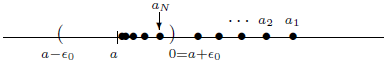
\includegraphics[width=0.6\linewidth]{figs/theorem2.3.4.png}
                    \caption{}
                \end{figure}\\ \\
                (ii) Assume that $a_n \leq b_n$ for $\forall n \in \mathbb{N}$. By the Algebraic Limit Theorem, $\lim(b_n-a_n)=b-a$. Since $b_n-a_n \geq 0$, by part (i), $b-a \geq 0 \implies a \leq b$.\\ \\
                (iii) Assume that there exists $c \in \mathbb{R}$ such that $c \leq b_n$ for $\forall n \in \mathbb{N}$. Since $\lim(b_n)=b$, by part (ii), let $a_n=c$ for $\forall n \in \mathbb{N}$, so $\lim(a_n)=\lim(c)=c$. Then,
                \begin{equation*}
                    c = a_n \leq b_n \implies c < b, \quad \forall n \in \mathbb{N}.
                \end{equation*}
                Similarly, assume that there exists $c \in \mathbb{R}$ such that $c \geq a_n$ for $\forall n \in \mathbb{N}$. Since $\lim(a_n)=a$, by part (ii), let $b_n=c$ for $\forall n \in \mathbb{N}$, so $\lim(b_n)=\lim(c)=c$. Then,
                \begin{equation*}
                    a_n \leq b_n = c \implies a < c, \quad \forall n \in \mathbb{N}.
                \end{equation*}
                QED
            
            \subsection{The Monotone Convergence Theorem and a First Look at Infinite Series}
                \fbox{\parbox{\linewidth}{\textbf{Definition 2.4.1.} A sequence $(a_n)$ is \textit{increasing} if $a_n \leq a_{n+1}$ for $\forall n \in \mathbb{N}$ and \textit{decreasing} if $a_n \geq a_{n+1}$ for $\forall n \in \mathbb{N}$. A sequence is \textit{monotone} if it is either increasing or decreasing.}}
                \\ \\
                \fbox{\parbox{\linewidth}{\textbf{Theorem 2.4.2 (Monotone Convergence Theorem).} \textit{If a sequence is monotone and bounded, then it converges.}}}
                \\ \\
                \textit{Proof.} Assume that $(a_n)$ is increasing and bounded, so $a_{n+1} \geq a_n$ and $|a_n| \leq M,M>0,\forall n \in \mathbb{N}$. Consider the set $\{a_n:n \in \mathbb{N}\}$. Since $(a_n)$ is bounded, by the Axiom of Completeness, there exists 
                \begin{equation*}
                    s = \sup \{a_n:n \in \mathbb{N}\}.
                \end{equation*}
                Since $s = \sup \{a_n:n \in \mathbb{N}\}$, therefore $\forall \epsilon>0,\exists N \in \mathbb{N}, s-\epsilon< a_N$. Because $a_{n+1} \geq a_n$, so if $n \geq N$, then $a_N \leq a_n$. Hence,
                \begin{gather*}
                    s-\epsilon<a_N\leq a_n \leq s < s+\epsilon\\
                    \therefore -\epsilon<a_n-s<\epsilon \implies |a_n-s|<\epsilon, n \geq N.
                \end{gather*}
                Thus, $\lim (a_n)=s$.\\ \\
                If $(a_n)$ is decreasing, then $a_{n+1}\leq a_n$. Because $(a_n)$ is bounded, by the Axiom of Completeness, there exists $i = \inf \{a_n:n\in \mathbb{N}\}$.\\ \\
                Since $i = \inf \{a_n:n\in \mathbb{N}\}$, therefore $\forall \epsilon>0, \exists N \in \mathbb{N}, i+\epsilon>a_N$. Because $a_{n+1} \leq a_n$, so if $n \geq N$, then $a_N \geq a_n$. Hence,
                \begin{gather*}
                    i+\epsilon > a_N \geq a_n > i-\epsilon \\
                    \therefore -\epsilon < a_n-i < \epsilon \implies |a_n-i| < \epsilon, n \geq N.
                \end{gather*}
                Thus, $\lim(a_n)=i.$\\ \\
                Therefore, if $(a_n)$ is monotone and bounded, then $(a_n)$ converges.\\ \\
                QED
                \begin{figure}[ht!]
                    \centering
                    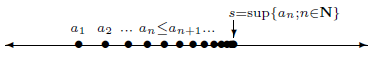
\includegraphics[width=0.6\linewidth]{figs/theorem 2.4.2.png}
                    \caption{Illustration of Theorem 2.4.2.}
                \end{figure}
                \\ \\
                \fbox{\parbox{\linewidth}{\textbf{Definition 2.4.3.} Let $(b_n)$ be a sequence. An \textit{infinite series} is a formal expression of the form
                \begin{equation*}
                    \sum_{n=1}^\infty b_n = b_1+b_2+b_3+\dots.
                \end{equation*}
                The corresponding \textit{sequence of partial sums} $(s_m)$ is defined as
                \begin{equation*}
                    s_m = b_1+b_2+\dots+b_m.
                \end{equation*}
                If $(s_m)$ converges to $B$, then the series $\sum_{n=1}^\infty b_n$ \textit{converges to} $B$,  written $\sum_{n=1}^\infty b_n = B$.}}
                \\ \\
                \textbf{Example 2.4.4.} Consider
                \begin{equation*}
                    \sum_{n=1}^\infty \frac{1}{n^2}.
                \end{equation*}
                Because the terms in the sum are all positive, the sequence of partial sums given by
                \begin{equation*}
                    s_m = 1 + \frac{1}{4} + \frac{1}{9} + \dots + \frac{1}{m^2}
                \end{equation*}
                is increasing. To find an upper bound on $(s_m)$, observe
                \begin{align*}
                    s_m & = 1 + \frac{1}{2\cdot2} + \frac{1}{3\cdot3} + \frac{1}{4\cdot4} + \dots + \frac{1}{m^2} \\
                    & < 1 + \frac{1}{2\cdot1} + \frac{1}{3\cdot2} + \frac{1}{4\cdot3} + \dots + \frac{1}{m(m-1)} \\
                    & = 1 + \bigg(1-\frac{1}{2}\bigg) + \bigg(\frac{1}{2}-\frac{1}{3}\bigg) + \bigg(\frac{1}{3}-\frac{1}{4}\bigg) + \dots + \bigg(\frac{1}{m-1}-\frac{1}{m}\bigg) \\
                    & = 1+1-\frac{1}{m} \\
                    & < 2.
                \end{align*}
                Thus, 2 is an upper bound for $(s_m)$, so by the Monotone Convergence Theorem, $\sum_{n=1}^\infty 1/n^2$ converges to some (presently unknown) limit less than 2.\\ \\
                \textbf{Example 2.4.5 (Harmonic Series).} Consider the \textit{harmonic series}
                \begin{equation*}
                    \sum_{n=1}^\infty \frac{1}{n}.
                \end{equation*}
                The sequence of partial sums 
                \begin{equation*}
                    s_m = 1 + \frac{1}{2} + \frac{1}{3} + \dots + \frac{1}{m}
                \end{equation*}
                is increasing. But 2 is not an upper bound because
                \begin{equation*}
                    s_4 = 1 + \frac{1}{2} + \bigg(\frac{1}{3}+\frac{1}{4}\bigg) > 1 + \frac{1}{2} + \bigg(\frac{1}{4}+\frac{1}{4}\bigg) = 2.
                \end{equation*}
                A similar calculation shows that $s_8 > 2\frac{1}{2}$, and in general
                \begin{align*}
                    s_{2^k} & = 1 + \frac{1}{2} + \bigg(\frac{1}{3}+\frac{1}{4}\bigg) + \bigg(\frac{1}{5}+\dots+\frac{1}{8}\bigg)+ \dots + \bigg(\frac{1}{2^{k-1}}+ \dots + \frac{1}{2^k}\bigg) \\
                    & > 1 + \frac{1}{2} + \bigg(\frac{1}{4}+\frac{1}{4}\bigg) + \bigg(\frac{1}{8}+\dots+\frac{1}{8}\bigg)+ \dots + \bigg(\frac{1}{2^k}+ \dots + \frac{1}{2^k}\bigg) \\
                    & = 1 + \frac{1}{2} + 2\bigg(\frac{1}{4}\bigg) + 4\bigg(\frac{1}{8}\bigg)+ \dots + 2^{k-1}\bigg(\frac{1}{2^k}\bigg) \\
                    & = 1 + \frac{1}{2} + \frac{1}{2} + \frac{1}{2} + \dots + \frac{1}{2} \\
                    & = 1 + k\bigg(\frac{1}{2}\bigg),
                \end{align*}
                which is unbounded. Thus, $(s_m)$ eventually surpasses every number on the positive real line. Because convergent sequences are bounded, the harmonic series diverges.
                \\ \\
                \fbox{\parbox{\linewidth}{\textbf{*Theorem 2.4.6 (Cauchy Condensation Test).} \textit{Suppose $(b_n)$ is decreasing and $b_n \geq 0$ for $\forall n \in \mathbb{N}$. Then, the series $\sum_{n=1}^\infty b_n$ converges if and only if the series}
                \begin{equation*}
                    \sum_{n=0}^\infty 2^n b_{2^n} = b_1 + 2b_2 + 4b_4 + 8b_8 + 16b_{16} + \dots
                \end{equation*}
                \textit{converges.}}}
                \\ \\
                \textit{Proof.} Suppose $(b_n)$ is decreasing and $b_n \geq 0$ for $\forall n \in \mathbb{N}$. Assume that $\sum_{n=1}^\infty 2^n b_{2^n}$ converges. By Theorem 2.3.2, the sequence of partial sums $(t_k)$ where
                \begin{equation*}
                    t_k = \sum_{n=0}^\infty 2^n b_{2^n} = b_1 + 2b_2 + 4b_4 + \dots + 2^kb_{2^k}
                \end{equation*}
                is convergent and bounded. Hence, $t_k \leq M$ for $M>0, \forall k \in \mathbb{N}$. Let
                \begin{equation*}
                    s_m = b_1+b_2+\dots+b_m
                \end{equation*}
                be the partial sum of $(b_n)$. Since $b_n \geq 0$, $(s_m)$ is increasing. \\ \\
                Fix $m$ and let $k$ be large enough such that $m \leq 2^{k+1}-1$. Then, $s_m \leq s_{2^{k+1}-1}$ and
                \begin{align*}
                    s_{2^{k+1}-1} & = b_1 + (b_2 + b_3) + (b_4 + b_5 + b_6 + b_7) + \dots + (b_{2^k} + \dots + b_{2^{k+1}-1}) \\ 
                    & \leq b_1 + (b_2 + b_2) + (b_4 + b_4 + b_4 + b_4) + \dots + (b_{2^k} + \dots + b_{2^k}) \\
                    & = b_1 + 2b_2 + 4b_4 + \dots + 2^kb_{2^k} \\
                    & = t_k.
                \end{align*}
                Hence, $s_m \leq s_{2^{k+1}-1} \leq t_k \leq M$, and $(s_m)$ is bounded. By the Monotone Convergence Theorem, since $(s_m)$ is monotone and bounded, $(s_m)$ converges. Thus, by Definition 2.4.3, $\sum_{n=1}^\infty b_n$ converges. \\ \\
                If $\sum_{n=0}^\infty 2^nb_n$ diverges, then $(t_k)$ diverges and is unbounded. Given an arbitrary $k \in \mathbb{N}$, consider $s_{2^k} \geq s_m$ such that
                \begin{align*}
                    s_{2^k} & = b_1 + b_2 + (b_3 + b_4) + (b_5 + b_6 + b_7 + b_8) + \dots + (b_{2^{k-1}+1} + \dots + b_{2^k}) \\
                    & \geq b_1 + b_2 + (b_4 + b_4) + (b_8 + b_8 + b_8 + b_8) + \dots + (b_{2^k} + \dots + b_{2^k}) \\
                    & = b_1 + b_2 + 2b_4 + 4b_8 + \dots + 2^{k-1}b_{2^k} \\
                    & = \frac{1}{2}(2b_1 + 2b_2 + 4b_4 + 8b_8 + \dots + 2^k b_{2^k}) \\
                    & = \frac{1}{2}\big(b_1 + (b_1 + 2b_2 + 4b_4 + 8b_8 + \dots + 2^k b_{2^k})\big) \\
                    & = \frac{1}{2}(b_1 + t_k) \\
                    & = \frac{b_1}{2} + \frac{t_k}{2}.
                \end{align*}
                Hence, there is a term $s_m \geq t_k/2$ for $\forall k \in \mathbb{N}$. Since $(t_k)$ is unbounded, $(s_m)$ is also unbounded and diverges. Hence, $\sum_{n=1}^\infty b_n$ diverges. \\ \\
                QED\\ \\
                \fbox{\parbox{\linewidth}{\textbf{*Corollary 2.4.7.} \textit{The series $\sum_{n=1}^\infty 1/n^p$ converges if an only if $p>1$.}}}
                \\ \\
                \textit{Proof.} Assume that $\sum_{n=1}^\infty 1/n^p$ converges. By the Cauchy Condensation Test, $\sum_{n=0}^\infty 2^n (1/2^n)^p$ converges. But
                \begin{align*}
                    \sum_{n=0}^\infty 2^n \bigg(\frac{1}{2^n}\bigg)^p &= \sum_{n=0}^\infty 2^n \bigg(\frac{1}{2^p}\bigg)^n \\
                    & = \sum_{n=0}^\infty \bigg(\frac{1}{2^{p-1}}\bigg)^n.
                \end{align*}
                Since the geometric series $\sum_{n=0}^\infty ar^n=a/(1-r),|r|<1$. So
                \begin{equation*}
                    \bigg|\frac{1}{2^{p-1}}\bigg| < 1 \implies \frac{1}{2^{p-1}} < 1 \implies 1 < 2^{p-1}.
                \end{equation*}
                Hence, $p>1$.\\ \\
                QED
            
            \subsection{Subsequences and the Balzano-Weierstrass Theorem}
                \fbox{\parbox{\linewidth}{\textbf{Definition 2.5.1.} Let $(a_n)$ be a sequence of real numbers, and let $n_1 < n_2 < n_3 < n_4 < n_5 < \dots$ be an increasing sequences of natural numbers. Then the sequence
                \begin{equation*}
                    a_{n_1}, a_{n_2}, a_{n_3}, a_{n_4}, a_{n_5}, \dots
                \end{equation*}
                is a \textit{subsequence} of $(a_n)$ denoted by $(a_{n_j})$, where $j \in \mathbb{N}$ indexes the subsequence.}}
                \\ \\
                
                The order of the terms in a subsequence is the same as in the original sequence, and repetitions are not allowed. If
                \begin{equation*}
                    (a_n) = \bigg(1, \frac{1}{2}, \frac{1}{3}, \frac{1}{4}, \frac{1}{5}, \frac{1}{6}, \dots \bigg),
                \end{equation*}
                then
                \begin{equation*}
                    \bigg(\frac{1}{2}, \frac{1}{4}, \frac{1}{6}, \frac{1}{8}, \dots \bigg) \quad \text{and} \quad \bigg(\frac{1}{10}, \frac{1}{100}, \frac{1}{1000}, \frac{1}{10000}, \dots \bigg)
                \end{equation*}
                are examples of subsequences, whereas
                \begin{equation*}
                     \bigg(\frac{1}{10}, \frac{1}{5}, \frac{1}{100}, \frac{1}{50}, \frac{1}{1000}, \frac{1}{500}, \dots \bigg) \quad \text{and} \quad \bigg(1,1,\frac{1}{3}, \frac{1}{5}, \frac{1}{7}, \frac{1}{9}, \dots \bigg)
                \end{equation*}
                are not.
                \\ \\
                \fbox{\parbox{\linewidth}{\textbf{Theorem 2.5.2.} \textit{Subsequences of a convergent sequence converge to the same limit as the original sequence.}}}
                \\ \\
                \textit{Proof.} Let $(a_n)$ be a convergent sequence, and let $(a_{n_j})$ be the subsequence of $(a_n)$. Since $(a_n)$ converges, 
                \begin{equation*}
                    \forall \epsilon > 0, \exists N \in \mathbb{N}: \forall n \geq N \implies |a_n-L|<\epsilon.
                \end{equation*}
                But $n_j \geq j$ (for example, if $a_{n_1} = a_1$, then $n_1 = 1$. If $a_{n_2} = a_5$, then $n_2=5 > 2$), so the same $N$ works for the subsequence as well. Hence, for $j \geq N$, it must be that $n_j \geq j \geq N$ and $|a_{n_j}-L|<\epsilon$.\\ \\
                QED\\ \\
                \textbf{Example 2.5.3.} Consider $(b^n) = (b,b^2,b^3,\dots)$. Let $0<b<1$, so
                \begin{equation*}
                    b>b^2>b^3>\dots>0
                \end{equation*}
                and $(b_n)$ is decreasing and bounded below. By the Monotone Convergence Theorem, $\lim(b_n)=L$ such that $b>L\geq 0$. Notice that 
                \begin{equation*}
                    (b^{2n}) = (b^2,b^4,b^6,\dots)
                \end{equation*}
                is a subsequence of $(b^n)$. Hence by Theorem 2.5.2, $\lim(b^{2n})=\lim(b^n)=L$. But by the Algebraic Limit Theorem,
                \begin{equation*}
                    \lim(b^{2n})=\lim(b^nb^n)=\lim(b^n)\lim(b^n)=L \cdot L=L^2.
                \end{equation*}
                Since limits are unique, $L^2=L \implies L=0$. Hence $\lim(b^n)=0$ for $0<b<1$. For $b=0,(b^n)=(0,0,0,\dots)$ and hence $\lim(b^n)=0$.\\ \\
                For $-1<b<0$, let $a=|b|$ so that $0<a<1$. Let $\epsilon>0$ be arbitrary, since $\lim(a^n)=0$, there exists $\exists N \in \mathbb{N}$ such that $|a^n-0|<\epsilon$. But this $N$ also works for $(b^n)$ because
                \begin{equation*}
                    |b^n-0|=|b^n|=|a^n|=|a^n-0|<\epsilon, \quad \forall n \geq N,
                \end{equation*}
                and $\lim(b^n)=0$ for $-1<b<0$. To generalize, $\lim(b^n)=0$ for $-1<b<1$.\\ \\
                \textbf{Example 2.5.4 (Divergence Criterion).} In Example 2.2.7, the sequence 
                \begin{equation*}
                    \bigg(1, -\frac{1}{2}, \frac{1}{3}, -\frac{1}{4}, \frac{1}{5}, -\frac{1}{5}, \frac{1}{5}, -\frac{1}{5}, \frac{1}{5}, -\frac{1}{5}, \frac{1}{5}, -\frac{1}{5}, \frac{1}{5}, -\frac{1}{5}, \frac{1}{5}, -\frac{1}{5}, \dots\bigg)
                \end{equation*}
                did not converge to any proposed limit. Notice that
                \begin{equation*}
                    \bigg(\frac{1}{5}, \frac{1}{5}, \frac{1}{5}, \frac{1}{5}, \frac{1}{5}, \dots\bigg)
                \end{equation*}
                is a subsequence that converges to 1/5. And 
                \begin{equation*}
                    \bigg(-\frac{1}{5}, -\frac{1}{5}, -\frac{1}{5}, -\frac{1}{5}, -\frac{1}{5}, \dots\bigg)
                \end{equation*}
                is another subsequence that converges to -1/5. Since there are two subsequences that converge to two different limits, the original sequence diverges.
                \\ \\
                \fbox{\parbox{\linewidth}{\textbf{Theorem 2.5.5 (Bolzano-Weierstrass Theorem)} \textit{Every bounded sequence contains a convergent subsequence.}}}
                \\ \\
                \textit{Proof.} Let $(a_n)$ be bounded, so there exists $M>0$ such that $|a_n|\leq M \implies a_n \in [-M,M]$ for $\forall n \in \mathbb{N}$. Bisect the closed interval $[-M,M]$ into two closed intervals $[-M,0]$ and $[0,M]$. It must be that one of the two closed intervals contains an infinite number of points in $(a_n)$. Select the half that this is true and call it $I_1$. Then, choose $a_{n_1} \in (a_n)$ such that $a_{n_1} \in I_1$.
                
                Next, bisect $I_1$ into two closed intervals of equal length, and let $I_2$ be the half that contains an infinite number of points of $(a_n)$. Choose $a_{n_2} \in (a_n)$ such that $n_2 > n_1$ and $a_{n_2} \in I_2$. In general, construct $I_k$ by taking a half of $I_{k-1}$ that contains an infinite number of points in $(a_n)$ and then choose $a_{n_k} \in (a_n)$ such that $n_k > n_{k-1} > \dots > n_2 > n_1$ and $a_{n_k} \in I_k$.
                \begin{figure}[ht!]
                    \centering
                    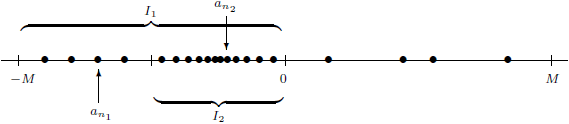
\includegraphics[width=0.8\linewidth]{figs/theorem2.5.5.png}
                    \caption{}
                \end{figure}
                
                The sets
                \begin{equation*}
                    I_1 \supseteq I_2 \supseteq I_3 \supseteq \dots
                \end{equation*}
                form a nested sequence of closed intervals. By the Nested Interval Property, $\cap_{k=1}^\infty I_k \neq \emptyset$ and there exists a point $x \in \mathbb{R}$ such that $x \in \cap_{k=1}^\infty I_k$.
                
                By construction, the lengths of $I_1,I_2,I_3,\dots$ are $M,M/2,M/2^2,\dots$, respectively. So the length of the length of $I_k$ is $M/2^{k-1}$. Consider the sequence
                \begin{equation*}
                    \bigg(\frac{1}{2^{k-1}}\bigg) = \bigg(1, \frac{1}{2}, \frac{1}{4}, \frac{1}{8}, \dots\bigg).
                \end{equation*}
                The sequence 
                \begin{equation*}
                    \bigg(\frac{1}{2^{2(k-1)}}\bigg) = \bigg(1, \frac{1}{4}, \frac{1}{16}, \dots\bigg)
                \end{equation*}
                is a subsequence of $(1/2^{k-1})$. By Theorem 2.5.2, $\lim(1/2^{k-1})=\lim(1/2^{2(k-1)})=L$. But by Algebraic Limit Theorem, 
                \begin{equation*}
                    \lim\bigg(\frac{1}{2^{2(k-1)}}\bigg) = \lim\bigg(\frac{1}{2^{k-1}}\frac{1}{2^{k-1}}\bigg) = \lim\bigg(\frac{1}{2^{k-1}}\bigg)\lim\bigg(\frac{1}{2^{k-1}}\bigg) = L \cdot L = L^2,
                \end{equation*}
                so $L^2 = L \implies L=0$ and $\lim(1/2^{k-1})=0$. Hence,
                \begin{equation*}
                    \lim\bigg(\frac{M}{2^{k-1}}\bigg)=\lim(M)\lim\bigg(\frac{1}{2^{k-1}}\bigg)=M\cdot 0=0.
                \end{equation*}
                So 
                \begin{equation*}
                    \forall \epsilon > 0, \exists N \in \mathbb{N}: \forall k \geq N \implies |(M/2^{k-1})-0|<\epsilon.
                \end{equation*}
                
                Let $\epsilon>0$ be arbitrary, choose an $N \in \mathbb{N}$ such that
                \begin{equation*}
                    \forall k \geq N \implies \frac{M}{2^{k-1}} < \epsilon.
                \end{equation*}
                Since $a_{n_k} \in I_k$ and $x \in I_k$, it follows that $|a_{n_k} - x| \leq M/2^{k-1} <\epsilon$.\\ \\
                QED
            
            \subsection{*The Cauchy Criterion}
            \textbf{Definition 2.6.1.} $(a_n)$ is a \textit{Cauchy sequence} if, for $\forall \epsilon >0$, there exists $\exists N \in \mathbb{N}$ such that $|a_n - a_m|<\epsilon$ whenever $m,n\geq N$.\\ \\
            \textbf{Theorem 2.6.2.} \textit{Every convergent sequence is a Cauchy sequence.}\\ \\
            \textit{Proof.} Suppose $(x_n)$ converges. So
            \begin{equation*}
                \forall \epsilon > 0, \exists N \in \mathbb{N}: |x_n-L|<\frac{\epsilon}{2},|x_m-L|<\frac{\epsilon}{2},\forall m, \forall n \geq N. 
            \end{equation*}
            By the Triangle Inequality,
            \begin{align*}
                |x_m-x_n| & = |x_m-L+L-x_n| \\
                & = |(x_m-L)+(L-x_n)| \\
                & \leq |x_m-L|+|L-x_n| \\
                & < \frac{\epsilon}{2} + \frac{\epsilon}{2} \\
                & = \epsilon, \forall m, \forall n \geq N.
            \end{align*}
            Hence, $(x_n)$ is a Cauchy sequence. \\ \\
            QED \\ \\
            \textbf{Lemma 2.6.3.} \textit{Cauchy sequences are bounded.}\\ \\
            \textit{Proof.} Suppose $(x_n)$ is a Cauchy sequence. Then for $\epsilon=1, \exists N \in \mathbb{N}: |x_m-x_n|<1, m,n\geq N$. Consider $|x_n - x_N|<1,n \geq N$, by the Reverse Triangle Inequality, $1 > |x_n-x_N| \geq |x_n|-|x_N| \implies |x_n| < |x_N|+1$. Let
            \begin{equation*}
                M>0:M = \max \{|x_1|,|x_2|,\dots,|x_{N-1}|,|x_N|+1\},
            \end{equation*}
            then $|x_n| < |x_N|+1 \leq M,\forall n \in \mathbb{N}$. Hence, $(x_n)$ is bounded.\\ \\
            QED\\ \\
            \textbf{Theorem 2.6.4 (Cauchy Criterion).} \textit{A sequence converges if and only if it is a Cauchy sequence.}\\ \\
            \textit{Proof.} ($\Rightarrow$) By, Theorem 2.6.2, every convergent sequence is a Cauchy sequence.\\ \\
            ($\Leftarrow$) Consider a Cauchy sequence $(x_n)$. By Lemma 2.6.3, $(x_n)$ is bounded. So by the Bolzano-Weierstrass Theorem, $(x_n)$ contains a convergent subsequence $(x_{n_k})$. Let
            \begin{equation*}
                \lim(x_{n_k})=x.
            \end{equation*}
            Since $(x_n)$ is a Cauchy sequence, \begin{equation*}
                \forall \epsilon > 0, \exists N \in \mathbb{N}: |x_n - x_m| < \epsilon, n,m \geq N.
            \end{equation*}
            Since $\lim(x_{n_k})=x$, choose a term in $(x_{n_k})$ such that
            \begin{equation*}
                \forall \epsilon>0,\exists N \in \mathbb{N}: |x_{n_k}-x|<\frac{\epsilon}{2}, \forall n_k \geq N.
            \end{equation*}
            If $n \geq n_k \geq N$, then
            \begin{equation*}
                |x_n - x_{n_k}| < \frac{\epsilon}{2}.
            \end{equation*}
            By the Triangle Inequality,
            \begin{align*}
                |x_n-x| & = |x_n - x_{n_k} + x_{n_k} - x| \\
                & = |(x_n - x_{n_k})+(x_{n_k} - x)| \\
                & \leq |x_n - x_{n_k}| + |x_{n_k} - x| \\
                & = \frac{\epsilon}{2} + \frac{\epsilon}{2} \\
                & = \epsilon, \forall n \geq N.
            \end{align*}
            QED
            \subsubsection{Completeness Revisited}
            \textbf{Proof that Axioms of Completeness and Nested Interval Property are equivalent.} Assume that the Nested Interval Property is true. Let $A$ be a non-empty set that is bounded above, and let $b_1$ be an upper bound for $A$. Next, choose an $a_1 \in \mathbb{R}$ that is not an upper bound of $A$. So $a_1 < b_1$. \\ \\
            Let $I_1 = [a_1,b_1]$. Next, bisect $I_1$ and let $c_1$ be the midpoint. If $c_1$ is an upper bound for $A$, then set $b_2=c_1$ and $a_2=a_1$. If $c_1$ is not an upper bound for $A$, then set $b_2=b_1$ and $a_2=c_1$. Let $I_2=[a_2,b_2]$, in either case described $a_2$ is not an upper bound for $A$ while $b_2$ is an upper bound for $A$.\\ \\
            Continuing the process, let $I_n = [a_n,b_n]$ and $c_n$ be the midpoint. If $c_n$ is an upper bound for $A$, then let $b_{n+1}=c_n$ and $a_{n+1}=a_n$. If $c_n$ is not an upper bound for $A$, then let $a_{n+1}=c_n$ and $b_{n+1}=b_n$. The resulting nested intervals
            \begin{equation*}
                I_1 \supseteq I_2 \supseteq \dots \supseteq I_n
            \end{equation*}
            has the property that, for every $n \in \mathbb{N}$, $a_n$ is not an upper bound while $b_n$ is an upper bound.\\ \\
            By the Nested Interval Property, there exists $s \in \mathbb{R}$ such that
            \begin{equation*}
                s \in \bigcap_{n=1}^\infty I_n.
            \end{equation*}
            Let $M=b_1-a_1$, so the length of $I_n$ is $M/2^{n-1}$ and $\lim(M/2^{n-1})=0$. So
            \begin{equation*}
                \forall \epsilon > 0, \exists N \in \mathbb{N}: \forall n \geq N \longrightarrow \bigg|\frac{M}{2^{n-1}}\bigg| < \epsilon.
            \end{equation*}
            Choosing $N$ such that $\forall n \geq N \longrightarrow M/2^{n-1} < \epsilon$. Since $a_n \in I_n$, $b_n \in I_n$, and $s \in I_n$,
            \begin{align*}
                \forall n \geq N & \longrightarrow |a_n - s| \leq M/2^{n-1} < \epsilon, |b_n - s| \leq M/2^{n-1} < \epsilon.
            \end{align*}
            Hence $\lim{a_n}=s$ and $\lim{b_n}=s$.\\ \\
            Let $a \in A$ be arbitrary. Since each $b_n$ is an upper bound, so $a \leq b_n, \forall n \in \mathbb{N}$. By the Order Limit Theorem, $a \leq s$. So $s$ is an upper bound for $A$.\\ \\
            Let $l$ be an arbitrary upper bound, so $a_n < l, \forall n \in \mathbb{N}$. By the Order Limit Theorem, $s \leq l$. So $s=\sup A$. Hence, $A$ is bounded above and has a least upper bound. This proved the Axioms of Completeness and shows that \textit{Nested Interval Property and Axioms of Completeness are equivalent}.\\ \\
            \textbf{Proof that Monotone Convergence Theorem and Nested Interval Property are equivalent.} Let $I_n = [a_n,b_n]$ be a collection of nested closed intervals. Since the intervals are nested, $(a_n)$ is increasing and bounded above (by $b_1$ for instance). By the Monotone Convergence Theorem, $\exists x \in \mathbb{R}:\lim(a_n)=x$. Fix $m \in \mathbb{N}$, so $a_m \leq x$. The nested property of the intervals also shows that $a_n \leq b_m, \forall n \in \mathbb{N}$, by the Order Limit Theorem, $x \leq b_m$. So $x \in \cap_{n=1}^\infty I_n$ and this proved the Nested Interval Property. This shows that \textit{Axioms of Completeness, Nested Interval Property, and Monotone Convergence Theorem are equivalent}.\\ \\
            \textbf{Proof that Bolzano-Weierstrass Theorem and Nested Interval Property are equivalent.} Let $I_n = [a_n,b_n]$ be a collection of nested closed intervals. $(a_n)$ may not converges but it is certainly bounded. By the Bolzano-Weierstrass Theorem, there exists a convergent subsequence $(a_{n_k})$. Let $\lim(a_{n_k})=x$. \\ \\
            Now fix $m \in \mathbb{N}$, since $a_{n_k} \leq b_m, \forall k \in \mathbb{N}$, by the Order Limit Theorem, $x \leq b_m$. Choosing a particular term $n_K \geq m$, it follows that $a_m \leq a_{n_K} \leq x$. Thus $x \in \cap_{m=1}^\infty I_m$. This proved the Nested Interval Property and shows that \textit{Axioms of Completeness, Nested Interval Property, Monotone Convergence Theorem, and Bolzano-Weierstrass Theorem are equivalent}.\\ \\
            \textbf{Proof that Cauchy Criterion and Bolzano-Weiersrass Theorem are equivalent.} Let $(a_n)$ be a bounded sequence so that $\exists M > 0 : |a_n| \leq M, \forall n \in \mathbb{N}$. Construct a sequence of closed intervals and the subsequence with $a_{n_k} \in I_k$ like in the proof of the Bolzano-Weierstrass Theorem. Let $\epsilon > 0$. The length of $I_k$ is $M(1/2)^{k-1}$ which converges to zero. Choose $N$ so that $k \geq N$ implies that the length of $I_k$ is less than $\epsilon$. So for any $s,t \geq N$, since $a_{n_s},a_{n_t} \in I_k$, it follows that $|a_{n_s} - a_{n_t}| < \epsilon$. Hence $(a_{n_k})$ is a Cauchy sequence and by the Cauchy Criterion, $(a_{n_k})$ converges. This proves the Bolzano-Weierstrass theorem and shows that \textit{Axioms of Completeness, Nested Interval Property, Monotone Convergence Theorem, Bolzano-Weierstrass Theorem, and Cauchy Criterion are equivalent}.
              
            \subsection{Properties of Infinite Series}
            \fbox{\parbox{\linewidth}{\textbf{Theorem 2.7.1 (Algebraic Limit Theorem for Series).} \textit{If $\sum_{k=1}^\infty a_k=A$ and $\sum_{k=1}^\infty b_k=B$, then}
            \begin{enumerate}[label=(\roman*)]
                \item $\sum_{k=1}^\infty ca_k = cA,\forall c \in \mathbb{R}$ \textit{(infinite additions are distributive) and}
                \item $\sum_{k=1}^\infty (a_k+b_k)=A+B$ \textit{(infinite series can be added in the usual way).}
            \end{enumerate}}}
            \\ \\
            \textit{*Proof.} (i) Suppose $\sum_{k=1}^\infty a_k = A$, so $\lim(s_m)=A$, where
            \begin{equation*}
                s_m = a_1 + a_2 + \dots + a_m.
            \end{equation*}
            Consider $\sum_{k=1}^\infty ca_k$ and its sequence of partial sums $(t_m)$, where 
            \begin{align*}
                t_m & = ca_1 + ca_2 + \dots + ca_m \\
                & = c(a_1+a_2+\dots+a_m) \\
                & = cs_m.
            \end{align*}
            So $(t_m)=(cs_m)$. By the Algebraic Limit Theorem,
            \begin{equation*}
                \lim(t_m) = \lim(cs_m) = \lim(c)\lim(s_m) = cA.
            \end{equation*}
            Hence, $\sum_{k=1}^\infty ca_k = cA$. \\ \\
            (ii) Assume that $\sum_{k=1}^\infty a_k=A, \sum_{k=1}^\infty b_k=B$. Let $(s_m)$ be the sequence of partial sums for $\sum_{k=1}^\infty a_k$ and $(t_m)$ be the partial sums for $\sum_{k=1}^\infty b_k$. So
            \begin{equation*}
                s_m = \sum_{k=1}^m a_k, t_m = \sum_{k=1}^m b_k.
            \end{equation*}
            To prove $\sum_{k=1}^\infty (a_k+b_k)=A+B$, it requires that the sequence of partial sum of $\sum_{k=1}^\infty (a_k+b_k)$ converges to $A+B$. Let $(r_m)$ be the sequence of partial sum of $\sum_{k=1}^\infty (a_k+b_k)$, so
            \begin{align*}
                r_m & = \sum_{k=1}^m (a_k+b_k) \\
                & = \sum_{k=1}^m a_k + \sum_{k=1}^m b_k \\
                & = s_m + t_m,
            \end{align*}
            and $\lim(r_m)=A+B$. By the Algebraic Limit Theorem, 
            \begin{equation*}
                \lim(r_m) = \lim(s_m+t_m) = \lim(s_m)+\lim(t_m) = A+B.
            \end{equation*}
            Hence, $\sum_{k=1}^\infty (a_k+b_k)=A+B$.
            \\ \\
            QED
            \\ \\
            \fbox{\parbox{\linewidth}{\textbf{*Theorem 2.7.2 (Cauchy Criterion for Series).} \textit{The series $\sum_{k=1}^\infty a_k$ converges if and only if, given $\epsilon>0$, there exists an $N \in \mathbb{N}$ such that}
            \begin{equation*}
                |a_{m+1} + a_{m+2} + \dots + a_n| < \epsilon, n>m \geq N.
            \end{equation*}}}
            \\ \\
            \textit{Proof.} 
            $(\Rightarrow)$ Assume that $\sum_{k=1}^\infty a_k = A$, so its sequence of partial sums $(s_m)$ converges. Hence,
            \begin{equation*}
                \forall \epsilon, \exists N \in \mathbb{N}: |s_m -A| < \frac{\epsilon}{2}, \forall m \geq N.
            \end{equation*}
            Let $n > m$, then
            \begin{equation*}
                |s_n -A| < \frac{\epsilon}{2}
            \end{equation*}
            and
            \begin{align*}
                |s_n - s_m| & = |(a_1+a_2+\dots+a_m+a_{m+1}+\dots +a_n)-(a_1+a_2+\dots+a_m)| \\
                & = |a_{m+1}+a_{m+2}+\dots+a_n|.
            \end{align*}
            But
            \begin{align*}
                |s_n - s_m| & = |s_n -A +A-s_m| \\
                & \leq |s_n-A|+|s_m-A| \\
                & < \frac{\epsilon}{2}+\frac{\epsilon}{2}\\
                & = \epsilon, n > m \geq N.
            \end{align*}
            Hence,
            \begin{equation*}
                |a_{m+1}+a_{m+2}+\dots+a_n| < \epsilon, n > m \geq N.
            \end{equation*}\\
            $(\Leftarrow)$ Consider the series $\sum_{k=1}^\infty a_k$ and its sequence of partial sums $(s_m)$. Assume 
            \begin{equation*}
                \forall \epsilon > 0, \exists N \in \mathbb{N}: |a_{m+1}+a_{m+2}+\dots+a_n|<\epsilon,n > m \geq N.
            \end{equation*}
            But
            \begin{align*}
                |a_{m+1}+a_{m+2}+\dots+a_n| & = |(a_1-a_1)+(a_2-a_2)+\dots+(a_m-a_m)+a_{m+1}+\dots+a_n| \\ 
                & = |(a_1+a_2+\dots+a_m+a_{m+1}+\dots+a_n)-(a_1+a_2+\dots+a_m)| \\
                & = |s_n - s_m| < \epsilon, n > m \geq N.
            \end{align*}
            So $(s_m)$ is a Cauchy sequence, and by Cauchy Criterion, $(s_m)$ converges. Hence, $\sum_{k=1}^\infty a_k$ converges.
            \\ \\
            \fbox{\parbox{\linewidth}{\textbf{*Theorem 2.7.3.} \textit{If the series $\sum_{k=1}^\infty a_k$ converges, then $\lim(a_k)=0$.}}}
            \\ \\
            \textit{Proof.} Assume $\sum_{k=1}^\infty a_k$ converges, then by Theorem 2.7.2, 
            \begin{equation*}
                \forall \epsilon > 0, \exists N \in \mathbb{N}: |a_{m+1}+a_{m+2}+\dots+a_n|<\epsilon,n > m \geq N.
            \end{equation*}
            Consider the special case $n=m+1$, so
            \begin{equation*}
                |a_n|=|a_n-0|<\epsilon,n \geq N.
            \end{equation*}
            Hence, $\lim(a_k)=0$.
            \\ \\
            QED
            \\ \\
            \fbox{\parbox{\linewidth}{\textbf{Theorem 2.7.4 (Comparison Test).} \textit{Assume $(a_k)$ and $(b_k)$ are sequences satisfying $0 \leq a_k \leq b_k,\forall k \in \mathbb{N}$}.
            \begin{enumerate}[label=(\roman*)]
                \item \textit{If $\sum_{k=1}^\infty b_k$ converges, then $\sum_{k=1}^\infty a_k$ converges.}
                \item \textit{If $\sum_{k=1}^\infty a_k$ diverges, then $\sum_{k=1}^\infty b_k$ diverges.}
            \end{enumerate}}}
            \\ \\
            \textit{Proof.} Assume $(a_k)$ and $(b_k)$ are sequences satisfying $0 \leq a_k \leq b_k,\forall k \in \mathbb{N}$. So
            \begin{equation*}
                |a_{m+1}+a_{m+2}+\dots+a_n| \leq |b_{m+1}+b_{m+2}+\dots+b_n|.
            \end{equation*}
            (i) If $\sum_{k=1}^\infty b_k$ converges, then by Cauchy Criterion for Series,
            \begin{equation*}
                \forall \epsilon > 0, \exists N \in \mathbb{N}: |b_{m+1}+b_{m+2}+\dots+b_n| < \epsilon,n>m \geq N.
            \end{equation*}
            Hence,
            \begin{equation*}
                |a_{m+1}+a_{m+2}+\dots+a_n| < \epsilon,n>m \geq N.
            \end{equation*}
            By Cauchy Criterion for Series, $\sum_{k=1}^\infty a_k$ converges.\\ \\
            (ii) If $\sum_{k=1}^\infty a_n$ diverges, then
            \begin{equation*}
                \exists \epsilon > 0, \forall N \in \mathbb{N}: |a_{m+1}+a_{m+2}+\dots+a_n| \geq \epsilon, n > m \geq N.
            \end{equation*}
            so 
            \begin{equation*}
                |b_{m+1}+b_{m+2}+\dots+b_n| \geq \epsilon, n > m \geq N.
            \end{equation*}
            By Cauchy Criterion for Series, $\sum_{k=1}^\infty b_k$ diverges. Alternatively, consider the contrapositive of the statement. If $\sum_{k=1}^\infty b_k$ converges, then $\sum_{k=1}^\infty a_k$ converges, which has been proven in (i). \\ \\
            Alternatively, using Monotone Convergence Theorem.\\
            (i) Let $t_n=\sum_{k=1}^n b_k,s_n=\sum_{k=1}^n a_k$. Since $0\leq a_k \leq b_k$, so $t_n \geq s_n$ and $(s_n)$ is bonded. Since $0\leq a_n$, $(s_n)$ is increasing. Hence, by the Monotone Convergence Theorem, $(s_n)$ converges and it follows that $\sum_{k-1}^\infty a_k$ converges.\\ \\
            (ii) Consider the contrapositive of the statement, which has been proven in (i).\\ \\
            QED\\ \\ 
            \textbf{Example 2.7.5 (Geometric Series).} A series is \textit{geometric} if it is of the form
            \begin{equation*}
                \sum_{k=1}^\infty ar^k = a + ar + ar^2 + ar^3 + \dots .
            \end{equation*}
            By the algebraic identity,
            \begin{equation*}
                (1-r)(1+r+r^2+r^3+\dots+r^{m-1})=1-r^m,
            \end{equation*}
            the partial sum can be rewritten as
            \begin{align*}
                s_m & = a + ar + ar^2 + ar^3 + \dots + ar^{m-1} \\ & = a(1+r+r^2+r^3+\dots+r^{m-1}) \\
                & = \frac{a(1-r^m)}{1-r}.
            \end{align*}
            By the Algebraic Limit Theorem,
            \begin{align*}
            \lim(s_m) & = \lim \bigg(\frac{a(1-r^m)}{1-r}\bigg) \\
            & = \lim(a) \lim \bigg(\frac{1-r^m}{1-r}\bigg) \\
            & = a \lim(1-r^m) \lim \bigg(\frac{1}{1-r}\bigg) \\
            & = \frac{a}{1-r}(1-\lim(r^m)).
            \end{align*}
            If $|r| \geq 1$, $\lim(r^m)$ diverges. If $|r|<1$, $\lim(r^m)=0$ and 
            \begin{align*}
                \lim(s_m) = \frac{a}{1-r}(1-0) = \frac{a}{1-r}.
            \end{align*}
            Hence the geometric series converges if and only if $|r| < 1$.
            \\ \\
            \fbox{\parbox{\linewidth}{\textbf{*Theorem 2.7.6 (Absolute Convergence Test).} \textit{If $\sum_{n=1}^\infty |a_n|$ converges, then $\sum_{n=1}^\infty a_n$ converges.}}}
            \\ \\
            \textit{Proof.} Assume $\sum_{n=1}^\infty |a_n|$ converges, so
            \begin{equation*}
                \forall \epsilon >0, \exists N \in \mathbb{N}: |a_{m+1}| + |a_{m+2}| + \dots + |a_n| < \epsilon, n > m \geq N.
            \end{equation*}
            By the triangle inequality,
            \begin{equation*}
                |a_{m+1}+a_{m+2}+\dots+a_n| \leq |a_{m+1}| + |a_{m+2}| + \dots + |a_n|.
            \end{equation*}
            Hence,
            \begin{equation*}
                |a_{m+1}+a_{m+2}+\dots+a_n| < \epsilon, n > m \geq N.
            \end{equation*}
            By Cauchy Criterion, $\sum_{n=1}^\infty a_n$ converges.\\ \\
            QED\\ \\
            \fbox{\parbox{\linewidth}{\textbf{*Theorem 2.7.7 (Alternating Series Test).} \textit{Let $(a_n)$ be a sequence satisfying}
            \begin{enumerate}[label=(\roman*)]
                \item $a_1 \geq a_2 \geq a_3 \geq \dots \geq a_n \geq a_{n+1} \geq \dots$ \textit{and}
                \item $\lim(a_n)=0$.
            \end{enumerate}
            \textit{Then, the alternating series $\sum_{n=1}^\infty (-1)^{n+1}a_n$ converges.}}}
            \\ \\
            \textit{Proof.} Consider the sequence of partial sums $(s_n)$ where
            \begin{equation*}
                s_n = a_1 - a_2 + a_3 - a_4 + \dots \pm a_n.
            \end{equation*}
            Since $\lim(a_n)=0$, so
            \begin{equation*}
                \forall \epsilon, \exists N \in \mathbb{N}: |a_n| < \epsilon > 0, n \geq N.
            \end{equation*}
            If $n>m$, then 
            \begin{align*}
                |s_n-s_m| & = |(a_1-a_2+\dots+a_m-a_{m+1}+\dots \pm a_n)-(a_1-a_2+\dots +a_m)| \\
                & = |a_{m+1}-a_{m+2}+\dots \pm a_n|.
            \end{align*}
            Since $(a_n)$ is decreasing and the terms $a_n$ are positive, 
            \begin{equation*}
                |a_{m+1}-a_{m+2}+\dots \pm a_n| \leq |a_{m+1}|.
            \end{equation*}
            If $n>m \geq N$, then
            \begin{equation*}
                |s_n-s_m| = |a_{m+1}-a_{m+2}+\dots \pm a_n|  \leq |a_{m+1}| < \epsilon, n>m \geq N.
            \end{equation*}
            So $(s_n)$ is Cauchy and converges. Hence, $\sum_{n=1}^\infty (-1)^{n-1} a_n$ converges.\\ \\
            Alternatively, let $I_1=[0,s_1],I_2=[s_2,s_1],\dots,I_k=[s_k,s_{k-1}],\dots$. So $I_1 \supseteq I_2 \supseteq \dots $ and by the Nested Interval Property Theorem, there exists an $S \in \bigcap_{k=1}^\infty I_k$.
            Consider $I_k=[s_k-s_{k-1}]$, its length is $|s_k - s_{k-1}|=|a_k|$. Since $\lim(a_n)=0$, so $|a_n|<\epsilon,n \geq N$. Since $s_k \in I_k,S \in I_k$, therefore
            \begin{equation*}
                |s_k-S| < |s_k-s_{k-1}|=|a_k|<\epsilon,k \geq N.
            \end{equation*}
            Hence, $(s_n)$ converges and $\sum_{n=1}^\infty (-1)^{n-1}a_n$ converges.\\ \\
            Alternatively, consider the subsequences $(s_{2n})$ and $(s_{2n+1})$ of $(s_n)$. Since $(a_n)$ is decreasing, $(s_{2n})$ is increasing and bounded ($s_{2n} \leq a_1$). Hence, by Monotone Convergence Theorem, $(s_{2n})$ converges. Let $\lim(s_{2n})=S$. Since $|a_n|<\epsilon,n \geq N$. By the Algebraic Limit Theorem,
            \begin{equation*}
                \lim(s_{2n+1}) = \lim(s_{2n} \pm a_{2n+1}) = \lim(s_{2n}) \pm \lim(a_{2n+1}) = S \pm 0 = S, n \geq N.
            \end{equation*}
            Since $\lim(s_{2n})=\lim(s_{2n+1})=S$, it follows that $\lim(s_n)=S$ and $\sum_{n=1}^\infty (-1)^{n-1}a_n$ converges.
            \\ \\
            QED
            \\ \\
            \fbox{\parbox{\linewidth}{\textbf{Definition 2.7.8.} If $\sum_{n=1}^\infty |a_n|$ converges, then $\sum_{n=1}^\infty a_n$ \textit{converges absolutely}. If $\sum_{n=1}^\infty a_n$ converges but $\sum_{n=1}^\infty |a_n|$ does not converge, then $\sum_{n=1}^\infty a_n$ \textit{converges conditionally}.}}
            
            \subsubsection{Rearrangements}
            \fbox{\parbox{\linewidth}{\textbf{Definition 2.7.9.} Let $\sum_{k=1}^\infty a_k$ be a series. A series $\sum_{k=1}^\infty b_k$ is a \textit{rearrangement} of $\sum_{k=1}^\infty a_k$ if there exists a one-to-one, onto function $f:\mathbb{N} \to \mathbb{N}$ such that $b_{f(k)}=a_k, \forall k \in \mathbb{N}$.}}
            \\ \\
            \fbox{\parbox{\linewidth}{\textbf{Theorem 2.7.10.} \textit{Let $\sum_{k=1}^\infty r_k$ be a rearrangement of the series $\sum_{k=1}^\infty$.}
            \begin{enumerate}[label=(\roman*)]
                \item \textit{If $\sum_{k=1}^\infty a_k$ converges absolutely, then any $\sum_{k=1}^\infty r_k$ converges to the same limit.}
                \item \textit{If $\sum_{k=1}^\infty a_k$ converges conditionally, then $\sum_{k=1}^\infty r_k$ can have different values and $\forall x \in \mathbb{R}, \exists \sum_{k=1}^\infty r_k = x$.}
            \end{enumerate}}}
            \\ \\
            \textit{Proof.} Assume $\sum_{k=1}^\infty a_k$ converges absolutely to $A$, and let $\sum_{k=1}^\infty b_k$ be a rearrangement of $\sum_{k=1}^\infty a_k$. So there exists a $f:\mathbb{N} \to \mathbb{N}$ such that $b_{f(k)} = a_k,\forall k \in \mathbb{N}$. Let 
            \begin{equation*}
                s_n = \sum_{k=1}^n = a_1+a_2+\dots+a_n
            \end{equation*}
            be the partial sums of $\sum_{k=1}^\infty a_k$ and 
            \begin{equation*}
                t_m = \sum_{k=1}^m = b_1+b_2+\dots+b_m
            \end{equation*}
            be the partial sums of $\sum_{k=1}^\infty b_k$.\\ \\
            Since $\sum_{k=1}^\infty a_k=A$, by Definition 2.4.3, $\lim(s_n)=A$. So
            \begin{equation*}
                \forall \epsilon >0, \exists N_1 \in \mathbb{N}: |s_n - A| < \frac{\epsilon}{2}, \forall n \geq N_1.
            \end{equation*}
            Since $\sum_{k=1}^\infty a_k$ converges absolutely, by Theorem 2.7.2, 
            \begin{equation*}
                \forall \epsilon > 0, \exists N_2 \in \mathbb{N}: \sum_{k=m+1}^n |a_k| < \frac{\epsilon}{2}, n>m \geq N_2.
            \end{equation*}
            Let $N=\max \{N_1,N_2\}$. Because $\sum_{k=1}^\infty b_k$ is a rearrangement of $\sum_{k=1}^\infty a_k$, the finite set of terms $\{a_1,a_2,\dots,a_N\}$ must all appear in $\sum_{k=1}^\infty b_k$. Let
            \begin{equation*}
                M = \max \{f(k): 1 \leq k \leq N\}.
            \end{equation*}
            So if $m \geq M$, then
            \begin{equation*}
                (t_m - s_N) = ((b_1+b_2+\dots+b_m)-(a_1+a_2+\dots+a_N))
            \end{equation*}
            consists of a finite set of terms, whose absolute values $|t_m - s_N|$ appear in $\sum_{k=N+1}^\infty |a_k|$. Hence, $|t_m - s_N| < \epsilon/2$ and by triangle inequality,
            \begin{align*}
                |t_m-A| & = |t_m-s_N+s_N-A| \\
                & \leq |t_m-s_N| + |s_N-A| \\
                & < \frac{\epsilon}{2} + \frac{\epsilon}{2} \\
                & = \epsilon, m \geq M.
            \end{align*}
            QED
            \\ \\
            \textbf{*Ratio Test.} \textit{Given $\sum_{n=1}^\infty a_n,a_n \neq 0$, if $(a_n)$ satisfies}
            \begin{equation*}
                \lim \bigg|\frac{a_{n+1}}{a_n}\bigg|=r<1,
            \end{equation*}
            \textit{then the series converges absolutely.}\\ \\
            \textit{Proof.} Since $\mathbb{R}$ is dense, there exists an $r'$ such that $r<r'<1$. Since $\lim|a_{n+1}/a_n|=r$, it must be that $|a_{n+1}/a_n|\in V_{\epsilon_0}(r), n \geq N.$ Let $\epsilon_0=|r-r'|$, so 
            \begin{equation*}
                \bigg|\frac{a_{n+1}}{a_n}\bigg| \leq r' \implies |a_{n+1}| \leq |a_n|r'.
            \end{equation*}
            Consider $|a_N|\sum_{n=1}^\infty (r')^n$. Since $\sum_{n=1}^\infty (r')^n$ is geometric and $|r'|<1$, the series converges. Now, since
            \begin{align*}
                |a_{N+1}| & \leq |a_N|r' \\
                |a_{N+2}| & \leq |a_{N+1}|r' \leq |a_n|(r')^2 \\
                & \vdots
            \end{align*}
            the series
            \begin{align*}
                \sum_{n=N+1}^\infty |a_n| & = |a_{N+1}| + |a_{N+2}| + \dots \\
                & \leq |a_N|r' + |a_N|(r')^2 + \dots \\
                & =|a_N|\sum_{n=1}^\infty (r')^n.
            \end{align*}
            By the comparison test, $\sum_{n=N+1}^\infty |a_n|$ converges. Since
            \begin{equation*}
                \sum_{n=1}^\infty |a_n| = \sum_{n=1}^N |a_n| + \sum_{n=N+1}^\infty |a_n|
            \end{equation*}
            and $\sum_{n=1}^N |a_n|$ is just a finite sum, $\sum_{n=1}^\infty |a_n|$ converges.
            \\ \\
            QED
            \\ \\
            \textbf{*Summation by Parts.} Let $(x_n)$ and $(y_n)$ be sequences, and $s_n = x_1 + \dots + x_n$. Using the observation that $x_j = s_j - s_{j-1}$,
            \begin{align*}
                s_n y_{n+1} - s_m y_{m+1} + \sum_{j=m+1}^n s_j(y_j-y_{j+1}) & = s_n y_{n+1} - s_m y_{m+1} + s_{m+1} (y_{m+1}-y_{m+2}) \\ 
                & + s_{m+2}(y_{m+2}-y_{m+3}) + \dots + s_{n}(y_{n}-y_{n+1}) \\
                & = s_n y_{n+1} - s_m y_{m+1} + s_{m+1} y_{m+1} - s_{m+1} y_{m+2} \\
                & + \dots + s_n y_n - s_n y_{n+1} \\
                & = (s_{m+1}-s_m)y_{m+1} + \dots + (s_n-s_{n-1}) y_n \\
                & = x_{m+1}y_{m+1} + \dots + x_n y_n \\
                & = \sum_{j=m+1}^n x_j y_j.
            \end{align*}
            \textbf{Dirichlet's Test.} \textit{If the partial sums of $\sum_{n=1}^\infty x_n$ are bounded (not necessarily convergent), and if $(y_n)$ is a sequence satisfying $y_1 \geq y_2 \geq \dots \geq 0$ with $\lim(y_n)=0$, then $\sum_{n=1}^\infty x_n y_n$ converges.}
            \\ \\
            \textit{Proof.} Let $M>0$ be an upper bound for the partial sums of $\sum_{n=1}^\infty x_n$, so $|s_n|<M$. By summation by parts,
            \begin{align*}
                \Bigg|\sum_{j=m+1}^n x_j y_j\Bigg| & = \Bigg|s_n y_{n+1} - s_m y_{m+1} + \sum_{j=m+1}^n s_j(y_j-y_{j+1})\Bigg| \\
                & \leq \Bigg|M y_{n+1} + M y_{m+1} + \sum_{j=m+1}^n M(y_j-y_{j+1})\Bigg| \\
                & = M \Bigg|y_{n+1} + y_{m+1} + \sum_{j=m+1}^n (y_j-y_{j+1})\Bigg| \\
                & = M |y_{n+1} + y_{m+1} + (y_{m+1}-y_{m+2}) + \dots + (y_n-y_{n+1})| \\
                & = M |2 y_{m+1}| \\
                & = 2M|y_{m+1}|.
            \end{align*}
            Since $\lim(y_n)=0$, for $\epsilon_0 = \epsilon/2M$, it must be that $|y_m|<\epsilon/2M,m \geq N$. Hence,
            \begin{equation*}
                \Bigg|\sum_{j=m+1}^n x_j y_j\Bigg| \leq 2M|y_{m+1}| < 2M (\frac{\epsilon}{2M}) = \epsilon, n > m \geq N.
            \end{equation*}
            By the Cauchy Criterion, $\sum_{j=1}^\infty x_j y_j$ converges.
            \\ \\
            QED
            \\ \\
            \textbf{*Abel's Test.} \textit{If $\sum_{n=1}^\infty x_n$ converges, and if $(y_n)$ is a sequence satisfying $y_1 \geq y_2 \geq \dots \geq 0$, then $\sum_{n=1}^\infty x_n y_n$ converges.}\\ \\
            \textit{Proof.} Assume that $\sum_{n=1}^\infty a_n$ has partial sums that are bounded by $A>0$, and $b_1 \geq b_ \geq \dots \geq 0$. By summation by parts,
            \begin{align*}
                \Bigg|\sum_{j=1}^n a_j b_j\Bigg| & = \Bigg|s_n b_{n+1} - s_m b_{m+1} + \sum_{j=m+1}^n s_j(b_j-b_{j+1})\Bigg| \\
                & \leq \Bigg|A b_{n+1} + A b_{m+1} + \sum_{j=m+1}^n A(b_j-b_{j+1})\Bigg| \\
                & = A \Bigg|b_{n+1} + b_{m+1} + \sum_{j=m+1}^n (b_j-b_{j+1})\Bigg| \\
                & = A |b_{n+1} + b_{m+1} + (b_{m+1}-b_{m+2})+\dots+(b_{n}-b_{n+1})| \\
                & = A|2b_{m+1}| \\
                & = 2A|b_{m+1}| \\
                & \leq 2Ab_1.
            \end{align*}
            Fix $m \in \mathbb{N}$ and let $a_n=x_{m+n},b_n=y_{m+n}$,
            \begin{align*}
                \Bigg|\sum_{j=m+1}^n x_j y_j\Bigg| & = |x_{m+1}y_{m+1} + x_{m+2}y_{m+2}+\dots+x_n y_n| \\
                & = |a_1b_1 + a_2b_2 + \dots + a_{n-m}b_{n-m}| \\
                & = \Bigg| \sum_{j=1}^{n-m} a_j b_j \Bigg| \\
                & \leq 2A_1b_1,
            \end{align*}
            where $A_1$ is an upper bound of the partial sums of $\sum_{j=m+1}^\infty x_j$, so $|\sum_{j=1}^n x_j| \leq A_1$. Since $\sum_{n=1}^\infty x_n$ converges, by the Cauchy Criterion,
            \begin{equation*}
                A_1 \leq \Bigg| \sum_{j=m+1}^n x_j \Bigg| < \frac{\epsilon}{2y_1}, n > m \geq N.
            \end{equation*}
            Since $b_1 = y_{m+1} \leq y_1$, 
            \begin{equation*}
                \Bigg|\sum_{j=m+1}^n x_j y_j\Bigg| \leq 2A_1b_1 < 2 \frac{\epsilon}{2y_1} y_1 = \epsilon, n > m \geq N.
            \end{equation*}
            Hence, by the Cauchy Criterion, $\sum_{j=1}^\infty x_j y_j$ converges.\\ \\
            QED
            \subsection{*Double Summations and Products of Infinite Series}
            \textbf{Theorem 2.8.1.} \textit{Let $\{a_{ij}:i,j \in \mathbb{N}\}$ be a doubly indexed array of real numbers. If}
            \begin{equation*}
                \sum_{i=1}^\infty \sum_{j=1}^\infty |a_{ij}|
            \end{equation*}
            \textit{converges, then}
            \begin{equation*}
                \sum_{i=1}^\infty \sum_{j=1}^\infty a_{ij} = \sum_{j=1}^\infty \sum_{i=1}^\infty a_{ji} = \lim_{n \to \infty} s_{nn},
            \end{equation*}
            \textit{where $s_{nn} = \sum_{i=1}^n \sum_{j=1}^n a_{ij}$.}\\ \\
            \textit{Proof.} Define the "rectangular partial sums" as
            \begin{equation*}
                s_{mn}=\sum_{i=1}^m\sum_{j=1}^n a_{ij}, \quad t_{mn}=\sum_{i=1}^m\sum_{j=1}^n |a_{ij}|.
            \end{equation*}
            Since $\sum_{i=1}^\infty \sum_{j=1}^\infty |a_{ij}|$ converges, it means that for every $i \in \mathbb{N},\sum_{j=1}^\infty |a_{ij}|=b_i,b_i \in \mathbb{R}$, and $\sum_{i=1}^m b_i$ converges. Now, 
            \begin{equation*}
                |t_{mn}| = \sum_{i=1}^m\sum_{j=1}^n |a_{ij}| \leq \sum_{i=1}^m\sum_{j=1}^\infty |a_{ij}| = \sum_{i=1}^m b_i \leq \sum_{i=1}^\infty b_i = L, L>0.
            \end{equation*}
            So $(t_{mn})$ is bounded and increasing, by the Monotone Convergence Theorem, $(t_{nn})$ converges and hence is a Cauchy sequence. Now,
            \begin{equation*}
                |s_{nn} - s_{mm}| \leq |t_{nn} - t_{mm}| < \epsilon, m,n \geq N.
            \end{equation*}
            So $(s_{nn})$ is a Cauchy sequence and it converges. Let
            \begin{equation*}
                \lim_{n \to \infty} s_{nn} = S.
            \end{equation*}
            Since $(t_{mn})$ is bounded, there exists
            \begin{equation*}
                B = \sup(t_{mn}).
            \end{equation*}
            Let $\epsilon > 0$ be arbitrary, there exists a point such that
            \begin{equation*}
                B-\frac{\epsilon}{2} < t_{m_0n_0} \leq B.
            \end{equation*}
            Since $(t_{mn})$ is increasing, for $m>m_0,n>n_0$,
            \begin{equation*}
                B-\frac{\epsilon}{2} < t_{m_0n_0} < t_{mn} \leq B.
            \end{equation*}
            Since $(t_{nn})$ is a Cauchy sequence, 
            \begin{equation*}
                \forall \epsilon > 0, \exists N_1 \in \mathbb{N} : |t_{mn} - t_{nn}| < \frac{\epsilon}{2}, n > m \geq N_1.
            \end{equation*} 
            Since $\lim_{n \to \infty} s_{nn} = S$,
            \begin{equation*}
                \forall \epsilon > 0, \exists N_2 \in \mathbb{N} : |s_{nn} - S| < \frac{\epsilon}{2},  n \geq N_2.
            \end{equation*}
            Let $N = max\{N_1,N_2\}$, then
            \begin{align*}
                |s_{mn}-S| & = |s_{mn} - s_{nn} + s_{nn} -S| \\
                & \leq |s_{mn} - s_{nn}| + |s_{nn} -S| \\
                & \leq |t_{mn} - t_{nn}| + |s_{nn} -S| \\
                & < \frac{\epsilon}{2} + \frac{\epsilon}{2} \\
                & = \epsilon, n>m \geq N.
            \end{align*}
            Since $\sum_{j=1}^\infty |a_{ij}| = b_i$ and $|a_{ij}| \geq a_{ij}$, it follows that $\sum_{j=1}^\infty a_{ij} = r_i,r_i \in \mathbb{N}$. Let $m \in \mathbb{N}$ be fixed, so
            \begin{equation*}
                s_{mn} = \sum_{j=1}^n a_{1j} + \sum_{j=1}^n a_{2j} + \dots + \sum_{j=1}^n a_{mj}.
            \end{equation*}
            By the Algebraic Limit Theorem,
            \begin{align*}
                \lim_{n \to \infty} s_{mn} & = \lim_{n \to \infty} \Bigg(\sum_{j=1}^n a_{1j} + \sum_{j=1}^n a_{2j} + \dots + \sum_{j=1}^n a_{mj}\Bigg) \\
                & = \sum_{j=1}^\infty a_{1j} + \sum_{j=1}^\infty a_{2j} + \dots + \sum_{j=1}^\infty a_{mj} \\
                & = r_1 + r_2 + \dots r_m.
            \end{align*}
            If $m \geq N$, then $|s_{mn} - S| < \epsilon$ is true eventually when $n \geq N$. Since $\lim_{n \to \infty} s_{mn} = r_1+\dots+r_m$ and $|s_{mn}-S| < \epsilon, n > m \geq N$, by the Order Limit Theorem,
            \begin{equation*}
                |(r_1+r_2+\dots+r_m)-S| \leq \epsilon, \forall m \geq N.
            \end{equation*}
            Since $\epsilon$ is arbitrary, a $\epsilon' < \epsilon$ can easily be chosen at the beginning and construct the argument using $\epsilon'$ throughout the proof. Hence, 
            \begin{equation*}
                \sum_{i=1}^\infty \sum_{j=1}^\infty a_{ij} = S.
            \end{equation*}
            Letting $n \in \mathbb{N}$ be fixed and hence
            \begin{align*}
                \lim_{m \to \infty} s_{mn} & = \lim_{m \to \infty} \Bigg( \sum_{i=1}^m a_{i1} + \sum_{i=1}^m a_{i2} + \dots + \sum_{i=1}^m a_{in} \Bigg) \\
                & = c_1 + c_2 + \dots c_n.
            \end{align*}
            Repeating the process,
            \begin{equation*}
                |(c_1 + c_2 + \dots c_n)-S| \leq \epsilon, \forall n \geq N,
            \end{equation*}
            and
            \begin{equation*}
                \sum_{j=1}^\infty \sum_{i=1}^\infty a_{ij} = S.
            \end{equation*}
            Hence,
            \begin{equation*}
                \sum_{i=1}^\infty \sum_{j=1}^\infty a_ij = \sum_{j=1}^\infty \sum_{i=1}^\infty a_{ij} = \lim_{n \to \infty} s_{nn} = S.
            \end{equation*}
            QED\\ \\
            Given a doubly indexed array $\{a_{ij}:i,j \in \mathbb{N}\}$, let
            \begin{equation*}
                d_2=a_{11}, d_3=a_{12}+a_{21},d_4=a_{13}+a_{22}+a_{31}
            \end{equation*}
            and in general
            \begin{equation*}
                d_k = a_{1,k-1}+a_{2,k-2}+\dots+a_{k-1,1}.
            \end{equation*}
            Then, $\sum_{k=2}^\infty d_k$ represents another way of summing over every $a_{ij}$ in the array. Let
            \begin{equation*}
                u_n = |d_2| + |d_3| + |d_4| + \dots + |d_n| = \sum_{k=2}^n |d_k|.
            \end{equation*}
            Since
            \begin{equation*}
                u_n = \sum_{k=2}^n |d_k| \leq \sum_{i=1}^n \sum_{j=1}^n |a_{ij}| = t_{nn},
            \end{equation*}
            and $(t_{nn})$ converges, by the Comparison Test, $(u_n)$ converges. Hence $\sum_{k=2}^\infty |d_k|$ converges and $\sum_{k=2}^\infty d_k$ converges absolutely.\\ \\
            From the proof of Theorem 2.8.1, $\lim_{n \to \infty} s_{nn} = S$, so
            \begin{equation*}
                \forall \epsilon > 0, \exists N_1 \in \mathbb{N} : \forall n \geq N_1 \longrightarrow |s_{nn}-S| < \frac{\epsilon}{2}.
            \end{equation*}
            Since $(t_nn)$ is a Cauchy sequence,
            \begin{equation*}
                \forall \epsilon > 0, \exists N_2 \in \mathbb{N} : \forall n > m \geq N_2 \longrightarrow |t_{nn}-t_{mm}| < \frac{\epsilon}{2}.
            \end{equation*}
            Let $N = \max \{N_1,2N_2\}$, then
            \begin{align*}
                \Bigg| \sum_{k=2}^n d_k -S \Bigg| & = \Bigg| \sum_{k=2}^n d_k - s_{nn} + s_{nn} - S \Bigg| \\
                & \leq \Bigg| \sum_{k=2}^n d_k - s_{nn} \Bigg| + |s_{nn} - S| \\ 
                & < \Bigg| \sum_{k=2}^n d_k - s_{nn} \Bigg| + \frac{\epsilon}{2}, \forall n \geq N.
            \end{align*}
            Since $n \geq 2N_2$, the partial sum $\sum_{k=2}^n d_k$ contains every term in $s_{N_2N_2}$. Therefore,
            \begin{equation*}
                \Bigg| \sum_{k=2}^n d_k - s_{nn} \Bigg| \leq (t_{nn} - t_{N_2N_2}) < \frac{\epsilon}{2}.
            \end{equation*}
            So
            \begin{equation*}
                \Bigg| \sum_{k=2}^n d_k -S \Bigg| < \frac{\epsilon}{2} + \frac{\epsilon}{2} = \epsilon, \forall n \geq N.
            \end{equation*}
            Hence, $\sum_{k=2}^\infty d_k = S$.
            
            \subsubsection{Products of Series}
            The product of two convergent series, called the \textit{Cauchy product}, is
            \begin{align*}
                \Bigg(\sum_{i=1}^\infty a_i\Bigg) \Bigg(\sum_{j=1}^\infty b_i\Bigg) & = (a_1 + a_2 + \dots)(b_1 + b_2 + \dots) \\
                & = a_1b_1 + (a_1b_2 + a_2b_1) + (a_3b_1 + a_2b_2 + a_1b_3) + \dots \\
                & = \sum_{k=2}^\infty d_k,
            \end{align*}
            where
            \begin{equation*}
                d_k = a_1b_{k-1}+a_2b_{k-2}+\dots+a_{k-1}b_1.
            \end{equation*}
            Assume that $\sum_{i=1}^\infty a_i$ converges absolutely to $A$ and $\sum_{j=1}^\infty b_j$ converges absolutely to $B$. Let
            \begin{equation*}
                \sum_{i=1}^\infty |a_i| = L, \sum_{j=1}^\infty |b_j| = M.
            \end{equation*}
            For each fixed $i \in \mathbb{N}$, by the Algebraic Limit Theorem,
            \begin{align*}
                \sum_{i=1}^\infty \sum_{j=1}^\infty |a_ib_j| & = |a_1|  \sum_{j=1}^\infty |b_j| + |a_2|  \sum_{j=1}^\infty |b_j| + \dots \\
                & = \sum_{i=1}^\infty |a_i|  \sum_{j=1}^\infty |b_j| \\
                & = \sum_{i=1}^\infty |a_i|M \\
                & = M\sum_{i=1}^\infty |a_i| \\
                & = ML.
            \end{align*}
            Let $s_{nn}=\sum_{i=1}^n \sum_{j=1}^n a_ib_j$, and let $i \in \mathbb{N}$ be fixed, by the Algebraic Limit Theorem,
            \begin{equation*}
                \lim_{n \to \infty} s_{nn} = \lim_{n \to \infty} \sum_{i=1}^n \sum_{j=1}^\infty a_ib_j =\lim_{n \to \infty} \Bigg(\sum_{i=1}^n a_i \Bigg) \Bigg(\sum_{j=1}^n b_j \Bigg) = AB.
            \end{equation*}
            Since $\sum_{i=1}^\infty \sum_{j=1}^\infty |a_ib_j|$ converges, by Theorem 2.8.1,
            \begin{equation*}
                \sum_{i=1}^\infty \sum_{j=1}^\infty a_ib_j = \sum_{j=1}^\infty \sum_{i=1}^\infty a_ib_j = \sum_{k=2}^\infty d_k = AB.
            \end{equation*}\\ \\
            
            \section{Basic Topology of $\mathbb{R}$}
            \subsection{Discussion: The Cantor Set}
            Let $C_0=[0,1]$, define $C_1$ as the set when the open middle third of $C_0$ is removed. So
            \begin{equation*}
                C_1 = C_0 \setminus \bigg(\frac{1}{3},\frac{2}{3}\bigg) = \bigg[0,\frac{1}{3}\bigg] \cup \bigg[\frac{2}{3},1\bigg].
            \end{equation*}
            Define $C_2$ by removing the open middle third of each of the two components of $C_1$,
            \begin{equation*}
                C_2 = \bigg(\bigg[0,\frac{1}{9}\bigg] \cup \bigg[\frac{2}{9},\frac{1}{3}\bigg]\bigg) \cup \bigg(\bigg[\frac{2}{3},\frac{7}{9}\bigg] \cup \bigg[\frac{8}{9},1\bigg]\bigg).
            \end{equation*}
            In general, for $n=0,1,2,\dots$, the set $C_n$ consists of $2^n$ closed intervals each having length $1/3^n$. Define the \textit{Cantor set} (Figure \ref{cantorset}) as
            \begin{equation*}
                C = \bigcap _{n=0}^\infty C_n .
            \end{equation*}
            \begin{figure}[ht!]
                \centering
                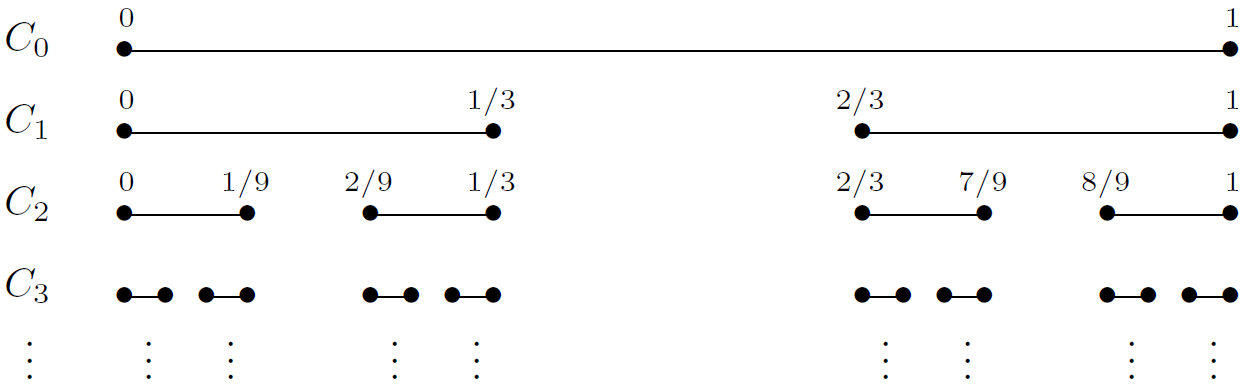
\includegraphics[width=0.9\linewidth]{figs/cantorset.png}
                \caption{Cantor set $C = \bigcap _{n=0}^\infty C_n$.}
                \label{cantorset}
            \end{figure}
            
            $C$ can be understand as the remainder of $[0,1]$ after the iterative process of removing open middle thirds is taken to infinity,
            \begin{equation*}
                C = [0,1] \setminus \bigg[\bigg(\frac{1}{3},\frac{2}{3}\bigg) \cup \bigg(\frac{1}{9},\frac{2}{9}\bigg) \cup \bigg(\frac{7}{9},\frac{8}{9}\bigg) \cup \dots \bigg].
            \end{equation*}
            Since the process always removes \textit{open} middle thirds, for $\forall n \in \mathbb{N}$, $0 \in C_n$ and hence $0 \in C$. Similarly, $1 \in C$. In general, if $y$ is the endpoint of some closed intervals of $C_n$, then it is also an endpoint of one of the intervals of $C_{n+1}$. Since endpoints are never removed at each stage, it follows that $y \in C_n, \forall n \in \mathbb{N}$. Thus, $C$ contains at least the endpoints of all of the intervals that make up each $C_n$.
            
            All of the endpoints mentioned earlier are rational numbers (the have the form $m/3^n$), so if $C$ only consists of these endpoints, then $C$ is a subset of $\mathbb{Q}$ and hence countable. If one considers the total length of the intervals removed, then there is not much left in $C$. To form $C_1$, an open interval of length $1/3$ was taken out. To form $C_2$, two intervals of length $1/9$ were removed. In general, to form $C_n$, $2^{n-1}$ middle thirds of length $1/3^n$ are removed. Then, the "length" of $C$ is
            \begin{equation*}
                1 - \bigg(\frac{1}{3}+ 2\bigg(\frac{1}{9}\bigg) + 4\bigg(\frac{1}{27}\bigg)+\dots+ 2^{n-1}\bigg(\frac{1}{3^n}\bigg)+\dots\bigg) = 1 - \frac{\frac{1}{3}}{1-\frac{2}{3}} = 1-1 =0.
            \end{equation*}
            $C$ has \textit{zero length}.
            
            If one creates a 1-1 correspondence between $C$ and $(a_n)_{n=1}^\infty$, where $a_n = 0$ or 1. For each $c \in C$, set $a_1=0$ if $c$ falls in the left-hand component of $C_1$ and $a_1=1$ if $c$ falls in the right-hand component. Having established where in $C_1$ the point $c$ is located, there are now two possible components of $C_2$ that might contain $c$. This time, set $a_2=0$ or 1 depending on whether $c$ falls in the left or right half of these two components of $C_2$. Continuing the process, $\forall c \in C$ yields $(a_1,a_2,a_3,\dots)$ of zeros and ones that acts as a set of directions for how to locate $c$ within $C$. Likewise, every such sequence corresponds to a point in $C$. Since the set of sequences of zeros and ones is uncountable, $C$ is \textit{uncountable} as well.
            
            Because the endpoints of $C_n$ form a countable set, it follows that not only are thee other points in $C$ but there are uncountably many of them. From the point of view of $cardinality$, $C$ is as large as $\mathbb{R}$. Contrasting with the point of view of $length$, $C$ measures the same size as a single point. 
            
            A point has dimension zero, a line segment has dimension one, a square has dimension two, and a cube has dimension three. Without attempting a formal definition of dimension, it might still can be defined by observing how the dimension affects the result of magnifying each particular set by a factor of 3 (Figure \ref{cantordim}). A single point undergoes no change at all, whereas a line segment triples in length. For the square, magnifying each length by a factor of 3 results in a larger square that contains 9 copies of the original square. Finally, the magnified cube yields a cube that contains 27 copies of the original cube within its volume. Notice that, in each case, to compute the “size” of the new set, the dimension appears as the exponent of the magnification factor.
            \begin{figure}[ht!]
                \centering
                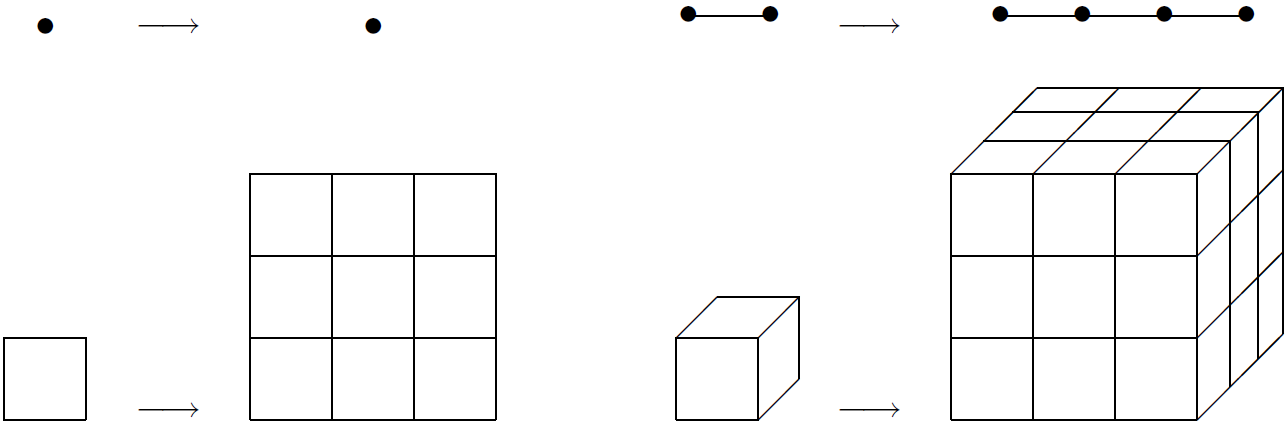
\includegraphics[width=0.8\linewidth]{figs/cantordim.png}
                \caption{Magnifying sets by a factor of 3.}
                \label{cantordim}
            \end{figure}
            
            Applying the same transformation to $C$. $C_0=[0,1]$ becomes $[0,3]$. Removing the open middle third leaves $[0,1]\cup[2,3]$, which is the original $C$ with an additional copy of $C$ in $[2,3]$. Magnifying $C$ by a factor of 3 yields \textit{two copies} of the original set. Thus, if $x$ is the dimension of $C$, then the size of $C$ after the transformation is $2=3^x$, or $x = \ln{2}/\ln{3} \approx 0.631$ (Figure \ref{cantorsize}).
            \begin{figure}[ht!]
                \centering
                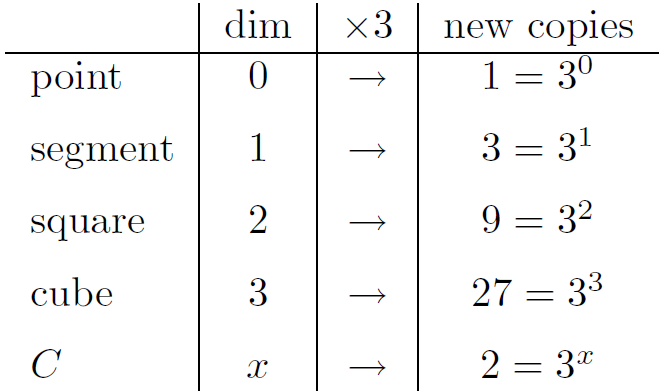
\includegraphics[width=0.45\linewidth]{figs/cantorsize.png}
                \caption{Dimension of $C$.}
                \label{cantorsize}
            \end{figure}
            
            Hence, from the point of view of length, $C$ has zero length. From the point of view of cardinality, $C$ is as large as $\mathbb{R}$. From the point of view of dimension, $C$ sits in between. 
            
            \subsection{Open and Closed Sets}
            \fbox{\parbox{\linewidth}{\textbf{Definition 3.2.1.} A set $O \subseteq \mathbb{R}$ is \textit{open} if $\forall a \in O, \exists \epsilon > 0 : V_\epsilon(a) = (a-\epsilon, a+\epsilon) \subseteq O.$}}
            \\ \\
            \textbf{Example 3.2.2.} (i) $\mathbb{R}$ is an open set. For an arbitrary $a \in \mathbb{R}$, one is free to pick any $\epsilon$-neighborhood and it will always be true that $V_\epsilon(a) \subseteq \mathbb{R}$. By the logical structure of Definition 3.2.1, the empty set $\emptyset$ is an open subset of the real line.
            
            (ii) Consider the open interval
            \begin{equation*}
                (c,d) = \{x \in \mathbb{R}: c < x < d\}.
            \end{equation*}
            Let $x \in (c,d)$ be arbitrary and $\epsilon = \min\{x-c,d-x\}$. If $\epsilon = x-c$, then \begin{equation*}
                V_\epsilon(x) = (x-(x-c), x+(x-c)) = (c, x+(x-c)).
            \end{equation*}
            Since $x+(x-c) < x+(d-x) = d$, it follows that $V_\epsilon(x) \subseteq (c,d)$. If $\epsilon = d-x$, then
            \begin{equation*}
                V_\epsilon(x) = (x-(d-x),x+(d-x)) = (x-(d-x),d).
            \end{equation*}
            Since $x-(d-x) > x-(x-c) = c$, it follows that $V_\epsilon(x) \subseteq (c,d)$.
            
            This argument breaks down if the interval includes either one of its endpoints since $\forall \epsilon > 0, V_\epsilon(c) \notin [c,d]$ and $V_\epsilon(d) \notin [c,d]$.
            \\ \\
            \fbox{\parbox{\linewidth}{\textbf{Theorem 3.2.3.} (i) \textit{The union of an arbitrary collection of open sets is open.}\\
            (ii) \textit{The intersection of a finite collection of open sets is open.}}}
            \\ \\
            \textit{Proof.} (i) Let $\{O_\lambda : \lambda \in \Lambda\}$ be a collection of open sets and $O = \bigcup_{\lambda \in \Lambda} O_\lambda$. Let $a \in O$ be arbitrary, so $a$ is an element of at least one particular open set $O_{\lambda'}$. Since $O_{\lambda'}$ is open, by Definition 3.2.1, there exists $V_\epsilon(a) \subseteq O_{\lambda'}$. Since $O_{\lambda'} \subseteq O$, it follows that $V_\epsilon(a) \subseteq O$. Hence, $O = \bigcup_{\lambda \in \Lambda} O_\lambda$ is open.
            
            (ii) Let $\{O_1, O_2, \dots, O_N\}$ be a finite collection of open sets and $O = \bigcap_{k=1}^N O_k$. Let $a \in O$, so $a$ is an element of each $O_k$. Since $O_k$ is open, for $1 \leq k \leq N$, there exists $V_{\epsilon_k}(a) \subseteq O_k$. To search for a \textit{single} $V_\epsilon$ that is contained in every $O_k$, let $\epsilon = \min\{\epsilon_1,\epsilon_2,\dots,\epsilon_N\}$. It follows that $V_\epsilon \subseteq V_{\epsilon_k}, \forall k$, and hence $V_\epsilon \subseteq \bigcap_{k=1}^N O_k$. Hence, $O = \bigcap_{k=1}^N O_k$ is open.\\ \\
            QED
            \subsubsection{Closed Sets}
            \fbox{\parbox{\linewidth}{\textbf{Definition 3.2.4.} A point $x$ is a \textit{limit point} of a set $A$ if $\exists a_n \in A, a_n \neq x: a_n \in V_\epsilon (x) \cap A, \forall \epsilon > 0.$}}
            \\ \\
            \fbox{\parbox{\linewidth}{\textbf{Theorem 3.2.5.} \textit{A point $x$ is a limit point of a set $A$ if and only if $x = \lim (a_n)$ for some sequence $(a_n)$ contained in $A$ satisfying $a_n \neq x, \forall n \in \mathbb{N}$.}}}
            \\ \\
            \textit{Proof.} $(\Rightarrow)$ Assume $x$ is a limit point of $A$. Consider $\epsilon = 1/n$, by Definition 3.2.4,
            \begin{equation*}
                a_n \in V_{1/n}(x) \cap A, \forall n \in \mathbb{N}, a_n \neq x.
            \end{equation*}
            Hence, $|a_n - x| < 1/n$. Let $\epsilon > 0$ be arbitrary, choose $N \in \mathbb{N}: n \geq N \implies 1/n \leq 1/N < \epsilon$. So , and hence $\forall n \geq N \implies |a_n - x| < 1/n \leq 1/N < \epsilon$. Hence, $\lim(a_n) = x$.
            \\ \\
            $(\Leftarrow)$ Assume that $\exists (a_n) \subseteq A, a_n \neq x: x=\lim(a_n)$. So 
            \begin{equation*}
                \forall \epsilon > 0, \exists N \in \mathbb{N}: a_n \in V_\epsilon(x), n \geq N.
            \end{equation*}
            Since $(a_n) \subseteq A$ and $a_n \in V_\epsilon(x)$, it follows that $V_\epsilon(x) \cap A = \{a_n\}, a_n \neq x, n \geq N$. Hence, $x$ is a limit point of $A$.\\ \\
            QED
            \\ \\
            \fbox{\parbox{\linewidth}{\textbf{Definition 3.2.6.} A point $a \in A$ is an \textit{isolated point of $A$} if it is not a limit point of $A$.}}
            \\ \\
            \fbox{\parbox{\linewidth}{\textbf{Definition 3.2.7} A set $F \subseteq \mathbb{R}$ is \textit{closed} if it contains all of its limit points.}}
            \\ \\
            \fbox{\parbox{\linewidth}{\textbf{Theorem 3.2.8.} \textit{A set $F \subseteq \mathbb{R}$ is closed if and only if every Cauchy sequence contained in $F$ has a limit that is also an element of $F$.}}}
            \\ \\
            \textit{Proof.} $(\Rightarrow) $. Assume $F \subseteq \mathbb{R}$ is closed, so $F$ contains its limit points. Let $(a_n) \subseteq F$ be a Cauchy sequence, so $(a_n)$ converges and $\lim(a_n) = x$ exists. If $a_n \neq x, \forall n \in \mathbb{N}$, then $x$ is a limit point of $F$ and hence $x \in F$. If $a_n = x, \exists n \in \mathbb{N}$, since $(a_n) \subseteq F$, it follows that $x \in F$. Hence, every Cauchy sequence contained in $F$ has a limit that is also an element of $F$.\\ \\
            $(\Leftarrow)$ Assume $\forall (a_n) \subseteq F$, $(a_n)$ is a Cauchy sequence, $\lim(a_n) = x \in F$. If $x$ is a limit point of $F$, then $\exists (a_n) \subseteq F: \lim(a_n) = x$. Since $\lim(a_n) = x \implies (a_n)$ is Cauchy, it follows that $x \in F$. Hence, $F$ contains its limit points and is closed. \\ \\
            QED\\ \\
            \textbf{Example 3.2.9.} (i) Consider
            \begin{equation*}
                A = \bigg\{\frac{1}{n}: n \in \mathbb{N}\bigg\}.
            \end{equation*}
            Given $1/n \in A$, choose $\epsilon = 1/n - 1/(n+1)$. Then,
            \begin{equation*}
                V_\epsilon(1/n) \cap A = \bigg\{\frac{1}{n}\bigg\}.
            \end{equation*}
            By Definition 3.2.4, $1/n$ is not a limit point and so is isolated. Although all of the points of $A$ are isolated, the set does have one limit point, namely 0. This is because every neighborhood centered at zero, no matter how small, is going to contain points of $A$. Because $0 \notin A$, $A$ is not closed. The set $F = A\cup\{0\}$ is an example of a closed set and is called the \textit{closure of} $A$.\\ \\
            (ii) Consider 
            \begin{equation*}
                [c,d] = \{x \in \mathbb{R}: c \leq x \leq d\}.
            \end{equation*}
            If $x$ is a limit point of $[c,d]$, then by Theorem 3.2.5 there exists $(x_n) \subseteq [c,d]$ with $\lim (x_n) = x$. By the Order Limit Theorem, since $c \leq x_n \leq d$, it follows that $c \leq x \leq d$. Thus, $[c,d]$ is closed.
            \\ \\
            \fbox{\parbox{\linewidth}{\textbf{Theorem 3.2.10 (Density of $\mathbb{Q}$ in $\mathbb{R}$).} \textit{Given any $y \in \mathbb{R}$, there exists a sequence of rational numbers that converges to y.}}}
            \\ \\
            \textit{Proof.} Consider the set $\mathbb{Q} \subseteq \mathbb{R}$ of rational numbers. Let $y \in \mathbb{R}$ be arbitrary, and consider any $V_\epsilon(y) = (y-\epsilon,y+\epsilon)$. By Theorem 1.4.3, there exists a rational number $r \neq y$ that falls in this neighborhood. Thus, $y$ is a limit point of $\mathbb{Q}$.
            
            By Theorem 3.2.5, since $y$ is a limit point of $\mathbb{Q}$, it follows that $y = \lim(r_n)$ for some sequence $(r_n)$ contained in $\mathbb{Q}$ satisfying $r_n \neq y, \forall n \in \mathbb{N}$.\\ \\
            QED
            \subsubsection{Closure}
            \fbox{\parbox{\linewidth}{\textbf{Definition 3.2.11} Given a set $A \subset \mathbb{R}$, let $L$ be the set of all limit points of $A$. The \textit{closure} of $A$ is defined as $\overline{A}=A \cup L$.}}
            \\ \\
            \fbox{\parbox{\linewidth}{\textbf{Theorem 3.2.12.} \textit{For any $A \subseteq \mathbb{R}$, the closure $\overline{A}$ is a closed set and is the smallest closed set containing $A$.}}}
            \\ \\
            \textit{Proof.} First prove that $L$ is closed. Let $A \subseteq \mathbb{R}$ and $L$ is the set of all limit points of $A$. Assume that $x$ is a limit point of $L$, so
            \begin{equation*}
                \exists l \in L, l \neq x: l \in V_\epsilon(x) \cap L, \forall \epsilon > 0.
            \end{equation*}
            Let $0 < \epsilon' < \epsilon$, $\epsilon'$ is small enough so that $V_{\epsilon'}(l) \subseteq V_\epsilon(x)$ and $x \notin V_{\epsilon'}(l)$. Since $l \in L$, $l$ is a limit point of $A$, so
            \begin{equation*}
                \exists a \in A, a \neq l: a \in V_{\epsilon'}(l) \cap A.
            \end{equation*}
            Hence, $a \in V_{\epsilon'}(l) \subseteq V_\epsilon(x) \implies a \in V_\epsilon(x)$ and $x$ is a limit point of $A$. Thus, $x \in L$ and $L$ is closed.
            
            Assume that $x$ is a limit point of $A \cup L$. So
            \begin{equation*}
                \exists l \in A \cup L, l \neq x: l \in V_\epsilon(x) \cap (A \cup L), \forall \epsilon > 0.
            \end{equation*}
            If $l \in V_\epsilon(x) \cap A$, then $x$ is a limit point of $A$ and $x \in L$. It follows that $x \in A \cup L$ and $A \cup L = \overline{A}$ is closed.
            
            If $l \in V_\epsilon(x) \cap L$, then let $\epsilon'$ be small enough so that $V_{\epsilon'}(l) \subseteq V_\epsilon(x)$ and $x \notin V_{\epsilon'}(l)$. Since $l \in L$, $l$ is a limit point of $A$ and 
            \begin{equation*}
                \exists a \in A, a \neq l: a \in V_{\epsilon'}(l) \cap A.
            \end{equation*}
            Hence, $a \in V_{\epsilon'}(l) \subseteq V_\epsilon(x) \implies a \in V_\epsilon(x)$ and $x$ is a limit point of $A$. Thus, $x \in L$ and $x \in A \cup L$, it follows that $A \cup L$ is closed.
            
            Now, let $F$ be a closed set and $A \subseteq F$. Since $A \subseteq F$ and $F$ is closed, $F$ contains all of the limit points of $A$. Hence $L \subseteq F$ and $\overline{A} = A \cup L$ is the smallest closed set containing $A$. 
            \\ \\
            QED
            
            \subsubsection{Complements}
            \fbox{\parbox{\linewidth}{\textbf{Theorem 3.2.13.} \textit{A set $O$ is open if and only if $O^c$ is closed. A set $F$ is closed if and only if $F^c$ is open.}}}
            \\ \\
            \textit{Proof.} $(\Rightarrow)$ Let $O \subseteq \mathbb{R}$ be an open set. To show that $O^c$ is closed, $O^c$ must contains all of its limit points. If $x$ is a limit point of $O^c$, then \textit{every} $V_\epsilon(x)$ contains some point of $O^c$. Since $O$ is open, $x \in O$ implies that there exists a $V_\epsilon(x) \subseteq O$, since every $V_\epsilon(x)$ contains some points of $O^c$, such neighborhood does not exist and it follows that $x \notin O$. Thus, $x \in O^c$ and $O^c$ is closed.
            
            $(\Leftarrow)$ Let $O^c$ be closed. To show that $O$ is open, $\forall x \in O, \exists \epsilon > 0: V_\epsilon(x) \subseteq O$. Let $x \in O$ be arbitrary. Because $O^c$ is closed and $x \notin O^c$, $x$ is not a limit point of $O^c$. By Definition 3.2.4, there must be some $V_\epsilon(x)$ that does not intersect $O^c$. But this means $V_\epsilon(x) \subseteq O$ and hence $O$ is open.
            
            The second statement follows from the first using the observation $(E^c)^c=E,\forall E \subseteq \mathbb{R}$.\\ \\
            QED
            \\ \\
            \fbox{\parbox{\linewidth}{\textbf{Theorem 3.2.14.} (i) \textit{The union of a finite collection of closed sets is closed.} (ii) \textit{The intersection of an arbitrary collection of closed sets is closed.}}}
            \\ \\
            \textit{Proof.} By De Morgan's Laws, given $\{E_\lambda : \lambda \in \Lambda\}$,
            \begin{equation*}
                \Bigg(\bigcup_{\lambda \in \Lambda} E_\lambda \Bigg)^c = \bigcap_{\lambda \in \Lambda} E^c_\lambda \quad \text{and} \quad \Bigg(\bigcap_{\lambda \in \Lambda} E_\lambda \Bigg)^c = \bigcup E^c_\lambda.
            \end{equation*}
            
            Let $x \in (\bigcup_{\lambda \in \Lambda} E_\lambda)^c$, so $x \notin \bigcup_{\lambda \in \Lambda} E_\lambda$. Hence $x \in E^c_\lambda, \forall \lambda$. So $x \in \bigcap_{\lambda \in \Lambda} E^c_\lambda$. Thus, $(\bigcup_{\lambda \in \Lambda} E_\lambda)^c \subseteq \bigcap_{\lambda \in \Lambda} E^c_\lambda$. Let $x \in \bigcap_{\lambda \in \Lambda} E^c_\lambda$, so $x \notin E_\lambda, \forall \lambda$. Hence $x \in (\bigcup_{\lambda \in \Lambda} E_\lambda)^c$ and $\bigcap_{\lambda \in \Lambda} E^c_\lambda \subseteq (\bigcup_{\lambda \in \Lambda} E_\lambda)^c$. Thus,
            \begin{equation*}
                \Bigg(\bigcup_{\lambda \in \Lambda} E_\lambda \Bigg)^c = \bigcap_{\lambda \in \Lambda} E^c_\lambda.
            \end{equation*}
            
            Let $x \in (\bigcap_{\lambda \in \Lambda} E_\lambda)^c$, so $x \notin \bigcap_{\lambda \in \Lambda} E_\lambda$. Hence there exists a $\lambda' \in \Lambda$ for which $x \notin E_{\lambda'}$ and $x \in E^c_{\lambda'}$. It follows that $x \in \bigcup_{\lambda \in \Lambda} E^c_\lambda$. Thus, $(\bigcap_{\lambda \in \Lambda} E_\lambda)^c \subseteq \bigcup_{\lambda \in \Lambda} E^c_\lambda$. Let $x \in \bigcup_{\lambda \in \Lambda} E^c_\lambda$, so there exists a $\lambda' \in \Lambda$ for which $x \in E^c_{\lambda'} \implies x \notin E_{\lambda'}$. It follows that $x \notin \bigcap_{\lambda \in \Lambda} E_\lambda \implies x \in (\bigcap_{\lambda \in \Lambda} E_\lambda)^c$. Hence $\bigcup_{\lambda \in \Lambda} E^c_\lambda \subseteq (\bigcap_{\lambda \in \Lambda} E_\lambda)^c$. Thus,
            \begin{equation*}
                \Bigg(\bigcap_{\lambda \in \Lambda} E_\lambda \Bigg)^c = \bigcup_{\lambda \in \Lambda} E^c_\lambda.
            \end{equation*}
            
            (i) Let $E_\lambda$ be a arbitrary collection of closed sets. By Theorem 3.2.13, $E^c_\lambda$ is a collection of open sets. By Theorem 3.2.3, $\bigcap_{\lambda \in \Lambda} E^c_\lambda$ is open. So
            \begin{equation*}
                \bigcap_{\lambda \in \Lambda} E^c_\lambda = \Bigg(\bigcup_{\lambda \in \Lambda} E_\lambda \Bigg)^c
            \end{equation*}
            is open. Hence, by Theorem 3.2.13, $\bigcup_{\lambda \in \Lambda} E_\lambda$ is closed.
            
            (ii) Let $E_\lambda$ be an arbitrary collection of closed sets. By Theorem 3.2.13, $E^c_\lambda$ is an arbitrary collection of open sets. By Theorem 3.2.3, $\bigcup_{\lambda \in \Lambda} E_\lambda$ is open. So
            \begin{equation*}
                \bigcup_{\lambda \in \Lambda} E^c_\lambda = \Bigg( \bigcap_{\lambda \in \Lambda} E_\lambda \Bigg)^c
            \end{equation*}
            is open. Hence by Theorem 3.2.13, $\bigcap_{\lambda \in \Lambda} E_\lambda$ is closed.\\ \\
            QED
            
            \subsection{Compact Sets}
            \fbox{\parbox{\linewidth}{\textbf{Definition 3.3.1 (Compactness).} A set $K \subseteq \mathbb{R}$ is \textit{compact} if $\forall (a_n) \subseteq K$ has a convergent subsequence $(a_{n_k}): \lim a_{n_k} = x$ and $x \in K$.}}
            \\ \\
            \textbf{Example 3.3.2} If $(a_n) \subseteq [c,d]$, then $(a_n)$ is bounded and by the Bolzano-Weierstrass Theorem, there exists a convergent subsequence $(a_{n_k})$. Because a closed interval is a closed set (Example 3.2.9 (ii)), the limit of $(a_{n_k})$ is also in $[c,d]$.
            
            $[0,\infty)$ is not compact since $(a_n)=n, \forall n \in \mathbb{N}$ does not have a convergent subsequence and $(a_n) \subseteq [0,\infty)$. Also, $\mathbb{R}, \mathbb{N}, \mathbb{Q}$ are not compact. $\{1/n: n \in \mathbb{N}\}$ is not compact since $(a_n) = (1/n) \to 0$ and $0 \notin \{1/n\}$.
            \\ \\
            \fbox{\parbox{\linewidth}{\textbf{Definition 3.3.3.} A set $A \subseteq \mathbb{R}$ is \textit{bounded} if $\exists M > 0: |a| \leq M, \forall a \in A$.}}
            \\ \\
            \fbox{\parbox{\linewidth}{\textbf{Theorem 3.3.4 (Characterization of Compactness in $\mathbb{R}$).} \textit{A set $K \subseteq \mathbb{R}$ is compact if and only if it is closed and bounded.}}}
            \\ \\
            \textit{Proof.} Logically, $K \subseteq \mathbb{R}$ is compact $\iff$ $K \subseteq \mathbb{R}$ is closed and bounded.
            \\ \\
            $(\Rightarrow)$ To show that $K$ is bounded. Let $K$ be compact. For the sake of contradiction, assume that $K$ is not bounded, so there must exist $x_1 \in K: |x_1| > 1$, $x_2 \in K: |x_2| > 2$, and in general, $x_n \in K: |x_n| > n, \forall n \in \mathbb{N}$. These points $x_n$ form a sequence $(x_n) \subseteq K$.
            
            Since $K$ is compact, by Definition 3.3.1, $(x_n)$ has a convergent subsequence $(x_{n_k})$ that converges to a point that is also in $K$. But the elements of $(x_{n_k})$ must satisfy $|x_{n_k}| > n_k$, so $(x_{n_k})$ is unbounded. Since by Theorem 2.3.2, convergent sequences are bounded, this is a contradiction. Hence, $K$ must be bounded.
            
            To show that $K$ is closed. Let $x$ be a limit point of $K$. So $\exists(x_n) \subseteq K: \lim x_n = x$. By Definition 3.3.1, since $K$ is compact, $(x_n)$ has a convegent subsequence $(x_{n_k})$ that coverges to a point that is also in $K$. By Theorem 2.5.2, $\lim x_n = x \implies \lim x_{n_k} = x$. Hence $x \in K$ and $K$ is closed.
            \\ \\
            $(\Leftarrow)$ Let $K \subseteq \mathbb{R}$ be closed and bounded. To show that $K$ is compact, $\forall (x_n) \subseteq K$, $(x_n)$ has a subsequence $(x_{n_k}): \lim x_{n_k} = x, x \in K.$ 
            
            Since $K$ is bounded, $\forall (x_n) \subseteq K$, $(x_n)$ is bounded. By the Bolzano-Weierstrauss Theorem, $(x_n)$ has a convergent subsequence $(x_{n_k})$. Let $\lim x_{n_k} = x$. Since $K$ is closed, $K$ contains all of its limit points. So $(x_{n_k}) \subseteq K, \lim x_{n_k} = x \implies x \in K$. Hence $K$ is compact. \\ \\
            QED
            \\ \\
            \fbox{\parbox{\linewidth}{\textbf{Theorem 3.3.5.} \textit{If $K_1 \supseteq K_2 \supseteq K_3 \supseteq \dots$ is a nested sequence of nonempty compact sets, then $\bigcap_{n=1}^\infty K_n$ is not empty.}}}
            \\ \\
            \textit{Proof.} Let $K_1 \supseteq K_2 \supseteq \dots$ be a nested sequence of compact sets. Choose $x_1 \in K_1, x_2 \in K_2, \dots$, and in general, $x_n \in K_n, \forall n \in \mathbb{N}$. These points form a sequence $(x_n)$. Since $K_1 \supseteq K_2 \supseteq \dots$, it follows that $(x_n) \subseteq K_1$. By Definition 3.3.1, since $K_1$ is compact, $(x_n)$ has a convergent subsequence $(x_{n_k}): \lim (x_{n_k}) = x, x \in K_1.$
            
            Consider the sequence $(x_2, x_3, \dots) \subseteq K_2$, it must contains the same subsequence $(x_{n_k}): \lim (x_{n_k}) = x, x \in K_2$. In general, let $n_0 \in \mathbb{N}$ be arbitrary, the terms in $(x_n)$ are contained in $K_{n_0}$ as long as $n \geq n_0$. Ignoring the finite number of terms for which $n_k < n_0$, the same subsequence $(x_{n_k})$ is also contained in $K_{n_0}$. Since $K_{n_0}$ is compact, $\lim (x_{n_k}) = x, x \in K_{n_0}$. Because $n_0$ is arbitrary, it follows that $x \in K_n, \forall n \in \mathbb{N}$. Hence, $x \in \bigcap_{n=1}^\infty K_n$.\\ \\
            QED
            
            \subsubsection{Open Covers}
            \fbox{\parbox{\linewidth}{\textbf{Definition 3.3.6.} Let $A \subseteq \mathbb{R}$. An \textit{open cover} for $A$ is a (possibly infinite) collection of open sets $\{O_\lambda : \lambda \in \Lambda\}$ satisfying $A \subseteq \bigcup_{\lambda \in \Lambda} O_\lambda$. A \textit{finite subcover} is a finite sub-collection of open sets $\{O_i\}_{i=1}^N \subseteq \{O_\lambda : \lambda \in \Lambda\}$ satisfying $A \subseteq \bigcup_{i=1}^N O_i$.}}
            \\ \\
            \textbf{Example 3.3.7.} Consider $(0,1)$. For each $x \in (0,1)$, let $O_x = (x/2,1)$. So 
            \begin{equation*}
                x \in O_x \implies x \in \bigcup_{x \in (0,1)} O_x, \forall x \in (0,1).
            \end{equation*}
            Hence, $(0,1) \subseteq \bigcup_{x \in (0,1)} O_x$ and $\{O_x: x \in (0,1)\}$ is an open cover for $(0,1)$. However, it is impossible to find a finite subcover for $(0,1)$. Given any $\{O_{x_1},O_{x_2},\dots,O_{x_n}\}$, let $x' = \min \{x_1,x_2,\dots,x_n\}$ and observe that $y \in \mathbb{R}, 0 < y \leq x'/2 \implies y \notin \bigcup_{i=1}^n O_{x_i}$. Hence, $(0,1) \nsubseteq \bigcup_{i=1}^n O_{x_i}$ and $\{O_{x_1},O_{x_2},\dots,O_{x_n}\}$ is not a finite subcover for $(0,1)$.
            
            \begin{figure}[ht!]
                \centering
                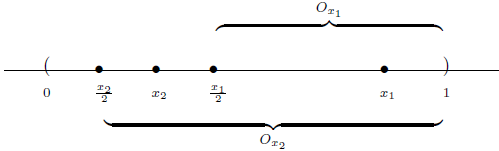
\includegraphics[width=0.8\linewidth]{figs/example3.3.7.png}
                \caption{}
            \end{figure}
            
            Consider $[0,1]$. Fix $\epsilon > 0$, and let $O_0 = (-\epsilon, \epsilon), O_1 = (1-\epsilon, 1+\epsilon)$ so that $0 \in O_0$ and $1 \in O_1$, and $O_x = (x/2, 1), \forall x \in (0,1)$.
            It follows that 
            \begin{equation*}
                \forall x \in [0,1], x \in O_0 \cup O_1 \cup \{O_x: x \in (0,1)\}
            \end{equation*}
            and hence $[0,1] \subseteq O_0 \cup O_1 \cup \{O_x: x \in (0,1)\}$. Therefore, $\{O_0, O_1, O_x: x \in (0,1)\}$ is an open cover for $[0,1]$. But this time, there is a finite subcover. Because of the addition of $O_0$, $x' \in (0,1)$ can be chosen so that $O_{x'} = (x'/2,1), x'/2 < \epsilon$. It follows that 
            \begin{equation*}
                x \in O_0 \cup O_{x'} \cup O_1, \forall x \in [0,1] \text{ and } [0,1] \subseteq O_0 \cup O_{x'} \cup O_1.
            \end{equation*}
            Hence $\{O_0,O_{x'},O_1\}$ is a finite subcover for $[0,1]$.
            \\ \\
            \fbox{\parbox{\linewidth}{\textbf{Theorem 3.3.8 (Heine-Borel Theorem).} \textit{Let $K \subseteq \mathbb{R}$. All of the following statements are equivalent in that any one of them implies the two others:}
            \begin{enumerate}[label=(\roman*)]
                \item \textit{$K$ is compact.}
                \item \textit{$K$ is closed and bounded.}
                \item \textit{Every open cover for $K$ has a finite subcover.}
            \end{enumerate}}}
            \\ \\
            \textit{Proof.} Theorem 3.3.4 shows that (i)$\iff$(ii). What is left is to show (ii)$\iff$(iii).
            \\ \\
            $(\Leftarrow)$ Assume that every open cover for $K \subseteq \mathbb{R}$ has a finite subcover. For the sake of contradiction, assume that $K$ is unbounded. So $K \subseteq \bigcup_{n=1}^\infty O_n$ and $K \nsubseteq \bigcup_{n=1}^N$. So $K$ does not have a finite subcover. This contradicts that every open cover of $K$ has a finite subcover. Hence, $K$ is bounded.
            
            To show that $K$ is closed, let $y$ be a limit point of $K$. So $\exists (a_n) \subseteq K: \lim a_n = y$. Assume that $y \notin K$. Define $O_{x_n} = V_{\frac{|x_n-y|}{2}}(x_n), \forall x_n \in F$. Since $y \notin K$, it follows that $F \subseteq \bigcup_{n=1}^\infty O_{x_n}$ and $F \nsubseteq \bigcup_{n=1}^N O_{x_n}$. This contradicts that $K$ has a finite subcover. Hence, $y \in K$ and $K$ is closed.
            \\ \\
            QED
            
            \subsection{Perfect Sets and Connected Sets}
            \subsubsection{*Perfect Sets}
            \subsubsection{Connected Sets}
            \fbox{\parbox{\linewidth}{\textbf{Definition 3.4.4.} Two nonempty sets $A,B \subseteq \mathbb{R}$ are \textit{separated} if $\overline{A} \cap B = \emptyset$ and $A \cap \overline{B} = \emptyset$. A set $E \subseteq \mathbb{R}$ is \textit{disconnected} if $E = A \cup B$, where $A$ and $B$ are nonempty separated sets. A set that is not disconnected is called a \textit{connected} set.}}
            \\ \\ \\
            \textbf{Example 3.4.5.} (i) Let $A = (1,2)$ and $B=(2,5)$, since $\overline{A} \cap B = \emptyset$ and $A \cap \overline{B} = \emptyset$, it follows that $E = (1,2) \cup (2,5)$ is disconnected. The sets $C = (1,2]$ and $D = (2,5)$ are not separated because $C \cap \overline{D} = {2}$. Hence the union $C \cup D = (1,5)$ is not disconnected.
            \\ \\
            (ii) Let
            \begin{equation*}
                A = \mathbb{Q} \cap (-\infty, \sqrt{2}) \quad \text{and} \quad B = \mathbb{Q} \cap (\sqrt{2}, \infty),
            \end{equation*}
            then $\mathbb{Q} = A \cup B$. By the Order Limit Theorem, since $A \subseteq (-\infty, \sqrt{2})$, it follows that any limit points of $A$ fall in $(\infty, \sqrt{2}]$. Hence $\overline{A} = (-\infty, \sqrt{2}]$ and $\overline{A} \cap B = \emptyset$. Similarly, $A \cap \overline{B} = \emptyset$. Hence, $A$ and $B$ are separated and $\mathbb{Q}$ is disconnected.
            \\
            
            Essentially, a set $E$ is connected if, no matter how it is partitioned into two nonempty disjoint sets, it is always possible to show that at least one of the sets contains a limit point of the other.
            \\ \\
            \fbox{\parbox{\linewidth}{\textbf{Theorem 3.4.6.*} \textit{A set $E \subseteq \mathbb{R}$ is connected if and only if, for all nonempty disjoint sets $A$ and $B$ satisfying $E = A \cup B$, there always exists a convergent sequence $(x_n) \to x$ with $(x_n)$ contained in one of $A$ or $B$, and $x$ an element of the other.}}}
            \\ \\
            \fbox{\parbox{\linewidth}{\textbf{Theorem 3.4.7.} \textit{A set $E \subseteq \mathbb{R}$ is connected if and only if whenever $a<c<b$ with $a,b \in E$, it follows that $c \in E$ as well.}}}
            \\ \\
            \textit{Proof.} $(\Rightarrow)$ Let $E \subseteq \mathbb{R}$ be a connected set. To show that $a,b \in E, a<c<b \implies c \in E$. For the sake of contradiction, assume that $a<c<b$ and $c \notin E$. Then, $E$ can be separated into two sets
            \begin{equation*}
                A = (-\infty,c) \cap E \quad \text{and} \quad B = (c,\infty) \cap E.
            \end{equation*}
            So
            \begin{equation*}
                \overline{A} = (-\infty,c] \cap E \quad \text{and} \quad \overline{B} = [c,\infty) \cap E.
            \end{equation*}
            It follows that
            \begin{equation*}
                \overline{A} \cap B = \emptyset \quad \text{and} \quad A \cap \overline{B} = \emptyset.
            \end{equation*}
            Hence $A$ and $B$ are separated and $E$ is disconnected. This contradicts that $E$ is connected. Therefore, $c \in E$.
            \\ \\
            QED
            
            \section{Functional Limits and Continuity}
            \subsection{Discussion: Examples of Dirichlet and Thomae}
            A function $f$ is continuous at $c$ if
            \begin{equation*}
                \lim_{x \to c} f(x) = f(c).
            \end{equation*}
            The Dirichlet's function is defined as
            \begin{equation*}
                g(x) = \bigg\{ \begin{matrix} 1 & ,x \in \mathbb{Q} \\ 0 & , x \notin \mathbb{Q}\end{matrix}.
            \end{equation*}
            \\
            \begin{figure}[ht!]
                \centering
                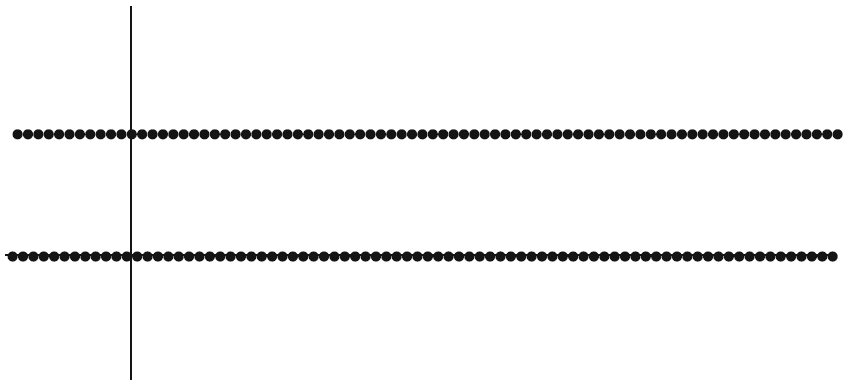
\includegraphics[width=0.6\linewidth]{figs/dirichlet.png}
                \caption{Dirichlet's Function.}
                \label{dirichlet}
            \end{figure}
            Consider a sequence $(x_n)$. If each $x_n$ is rational, then
            \begin{equation*}
                \lim_{n \to \infty} g(x_n) = 1.
            \end{equation*}
            If each $x_n$ is irrational, then
            \begin{equation*}
                \lim_{n \to \infty} g(x_n) = 0.
            \end{equation*}
            Because $\mathbb{Q}$ and $\mathbb{I}$ are dense in the real line, it follows that $\forall z \in \mathbb{R}, \exists (x_n) \subseteq \mathbb{Q}, \exists (y_n) \subseteq \mathbb{I}$ such that
            \begin{equation*}
                \lim x_n = \lim y_n = z.
            \end{equation*}
            Since
            \begin{equation*}
                \lim g(x_n) \neq \lim g(y_n),
            \end{equation*}
            $g(x)$ is not continuous at $z$. Hence the Dirichlet's function is a \textit{nowhere-continuous} function on $\mathbb{R}$.
            \\ \\
            Define a Modified Dirichlet's function
            \begin{equation*}
                h(x) = \bigg\{ \begin{matrix}x &, x \in \mathbb{Q} \\ 0 &, x \notin \mathbb{Q} \end{matrix}.
            \end{equation*}
            Let $c \neq 0, (x_n) \subseteq \mathbb{Q}, (y_n) \subseteq \mathbb{I}: (x_n) \to c, (y_n) \to c$. It follows that
            \begin{equation*}
                \lim h(x_n) = c \neq \lim h(y_n) = 0.
            \end{equation*}
            Thus, $h$ is not continuous at $\forall c \neq 0$.
            \\ \\
            If $c=0$, then
            \begin{equation*}
                \lim h(x_n) = \lim h(y_n) = 0.
            \end{equation*}
            In fact, $\forall (z_n) \to 0, \lim h(z_n) = 0$. Thus,
            \begin{equation*}
                \lim_{x \to c} h(x) = L \implies h(z_n) \to L, \forall (z_n) \to c.
            \end{equation*}
            
            \begin{figure}[ht!]
                \centering
                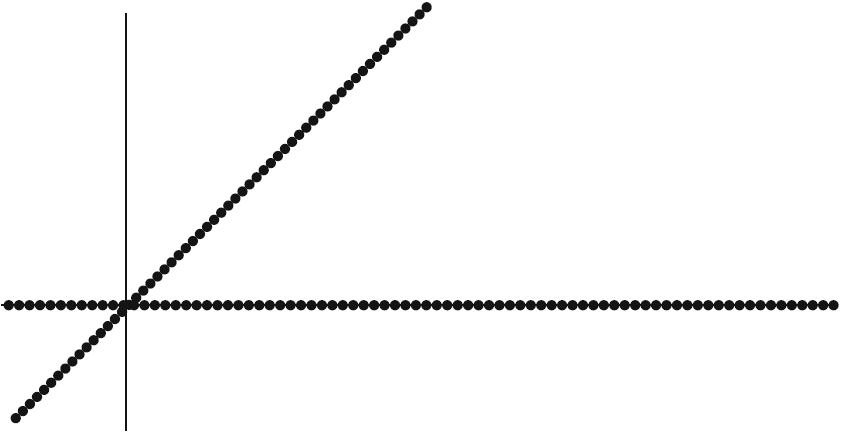
\includegraphics[width=0.6\linewidth]{figs/modified dirichlet.png}
                \caption{Modified Dirichlet's Function.}
                \label{dirichlet}
            \end{figure}
            
            \subsection{Functional  Limits}
            \fbox{\parbox{\linewidth}{\textbf{Definition 4.2.1 (Functional Limit).} Let $f:A \to \mathbb{R}$, and let $c$ be a limit point of the domain $A$. Then $\lim_{x \to c} f(x) = L$ provided that
            \begin{equation*}
                \forall \epsilon > 0, \exists \delta > 0: 0 < |x-c| < \delta \implies |f(x)-L|<\epsilon.
            \end{equation*}}}
            \\ \\
            The additional restriction $0 < |x-c|$ is saying that $x \neq c$.
            \\ \\ \fbox{\parbox{\linewidth}{\textbf{Definition 4.2.1B (Functional Limit: Topological Version).} Let $c$ be a limit point of the domain of $f: A \to \mathbb{R}$. Then $\lim_{x \to c} f(x) = L$ provided that
                \begin{equation*}
                    \forall \epsilon > 0, \exists \delta > 0: \forall x \in V_\delta (c), x \neq c \implies f(x) \in V_\epsilon(L).
                \end{equation*}
            }}
            \begin{figure}[ht!]
                \centering
                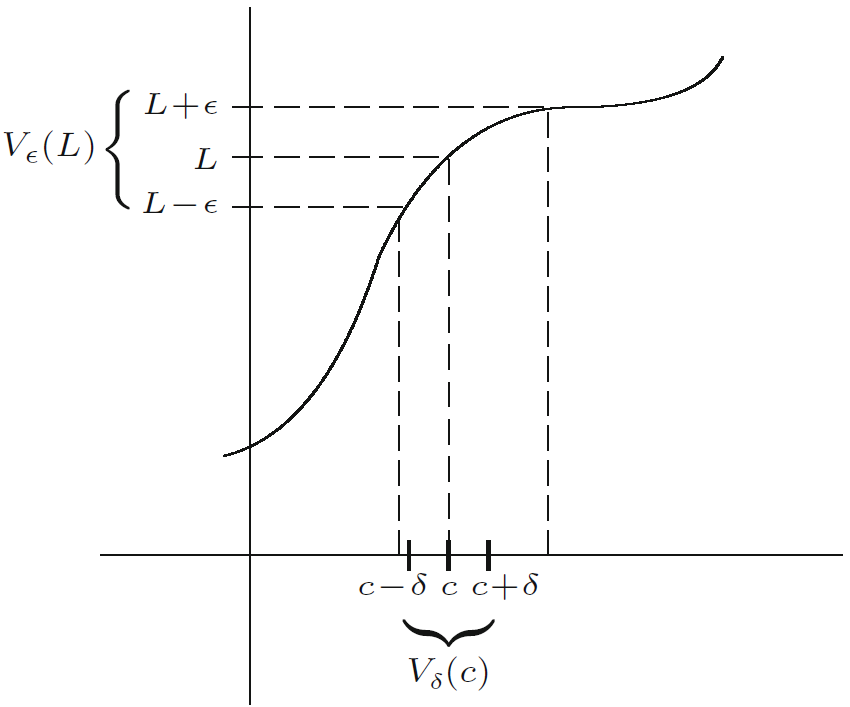
\includegraphics[width=0.6\linewidth]{figs/functional_limit.png}
                \caption{Definition of Functional Limit.}
                \label{functional_limit}
            \end{figure}
            \\ \\
            \textbf{Example 4.2.2.} (i) Prove that if $f(x)=3x+1$, then
            \begin{equation*}
                \lim_{x \to 2} f(x) = 7.
            \end{equation*}
            WTS:
            \begin{equation*}
                \forall \epsilon > 0, \exists \delta > 0: 0<|x-2|<\delta \implies |(3x+1)-7|<\epsilon.
            \end{equation*}
            Notice that
            \begin{equation*}
                |(3x+1)-7| = |3x+1-7| = |3x-6| = 3|x-2| < \epsilon \implies |x-2| < \frac{\epsilon}{3}.
            \end{equation*}
            Let $\epsilon>0$, and let $\delta = \epsilon/3$. Then \begin{equation*}
                0 < |x-2| < \delta \implies |(3x+1)-7| = 3|x-2| < 3 \delta = 3\bigg(\frac{\epsilon}{3}\bigg) = \epsilon,
            \end{equation*}
            as desired.
            \\ \\
            (ii) Prove that if $g(x)=x^2$, then
            \begin{equation*}
                \lim_{x \to 2} g(x) = 4.
            \end{equation*}
            WTS:
            \begin{equation*}
                \forall \epsilon > 0, \exists \delta > 0: 0<|x-2|<\delta \implies |x^2-4|<\epsilon.
            \end{equation*}
            Notice that
            \begin{align*}
                |x^2 - 4| & = |(x+2)(x-2)| \\
                & = |x+2| |x-2|.
            \end{align*}
            Since $0<|x-2|<\delta$, $x$ is close to 2. Let $\delta < 1$, so $x<2+1=3$, then
            \begin{align*}
                |x^2-4| & = |x+2| |x-2| \\
                & < |3+2| |x-2| \\
                & = 5|x-2| \\
                & < \epsilon \\ 
                \therefore |x-2| & < \frac{\epsilon}{5}.
            \end{align*}
            Let $\epsilon>0, \delta=\min\{1,\epsilon/5\}$, then
            \begin{equation*}
                0<|x-2|<\delta \implies |x^2-4| < 5|x-2| < 5\bigg(\frac{\epsilon}{5}\bigg) = \epsilon,
            \end{equation*}
            as desired.
            
            \subsubsection{Sequential Criterion for Functional Limits}
            \fbox{\parbox{\linewidth}{\textbf{Theorem 4.2.3 (Sequential Criterion for Functional Limits).} \textit{Given a function $f:A \to \mathbb{R}$ and a limit point $c$ of $A$, the following are equivalent:}
            \begin{enumerate}[label=(\roman*)]
                \item $\lim_{x \to c} f(x) = L.$
                \item \textit{For all sequences $(x_n) \subseteq A$ satisfying $x_n \neq c$ and $(x_n) \to c$, it follows that $f(x_n) \to L.$}
            \end{enumerate}
            }}
            \\ \\
            \fbox{\parbox{\linewidth}{\textbf{Corollary 4.2.4 (Algebraic Limit Theorem for Functional Limits)} \textit{Let $f$ and $g$ be functions defined on a domain $A \subseteq \mathbb{R}$, and assume $\lim_{x \to c} f(x) = L$ and $\lim_{x \to c} g(x) = M$ for some limit point $c$ of $A$. Then}
            \begin{enumerate}[label=(\roman*)]
                \item $\lim_{x \to c} kf(x) = kL, \forall k \in \mathbb{R}$,
                \item $\lim_{x \to c} |f(x) + g(x)| = L+M$,
                \item $\lim_{x \to c} |f(x)g(x)| = LM$,
                \item $\lim_{x \to c} f(x)/g(x) = L/M, M \neq 0$.
            \end{enumerate}
            }}
            \\ \\
            \fbox{\parbox{\linewidth}{\textbf{Corollary 4.2.5 (Divergence Criterion for Functional Limits).} \textit{Let $f$ be a function defined on $A$, and let $c$ be a limit point of $A$. If there exists two sequences $(x_n)$ and $(y_n)$ in $A$ with $x_n \neq c$ and $y_n \neq c$ and}
            \begin{equation*}
                \lim x_n = \lim y_n \quad \text{but} \quad \lim f(x_n) \neq \lim f(y_n),
            \end{equation*}
            then the functional limit $\lim_{x \to c} f(x)$ does not exist.
            }}
            \\ \\
            \textbf{Example 4.2.6.} Show that $\lim_{x \to 0} \sin{1/x}$ does not exist.
            \\
            Let $(x_n) = (1/2n\pi)$ and $(y_n)=1/(2n\pi + \pi/2)$, then $\lim (x_n) = \lim (y_n) = 0$. But $\sin(1/x_n) = \sin(2n\pi) = 0$ and $\sin(1/y_n) = \sin(2n\pi + \pi/2) = 1, \forall n \in \mathbb{N}$. So $\lim \sin(1/x_n) \neq \lim \sin(1/_n)$ and by Corollary 4.2.5, $\lim_{x \to 0} \sin(1/x)$ does not exist.
            
            \begin{figure}[ht!]
                \centering
                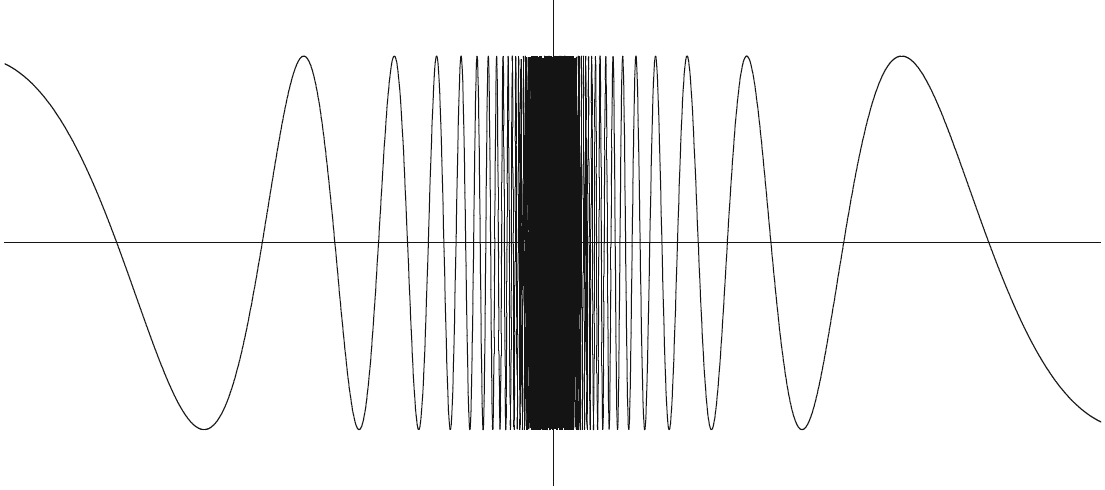
\includegraphics[width=0.8\linewidth]{figs/sinx^-1.png}
                \caption{The function $\sin(1/x) near zero.$}
                \label{sin1/x}
            \end{figure}
            
            \subsection{Continuous Functions}
            \fbox{\parbox{\linewidth}{\textbf{Definition 4.3.1 (Continuity).} A function $f:A \to \mathbb{R}$ is \textit{continuous at a point} $c \in A$ if
            \begin{equation*}
                \forall \epsilon >0, \exists \delta >0: 0<|x-c|<\delta \implies |f(x)-f(c)|<\epsilon,
            \end{equation*}.
            }}
            \\ \\
            \fbox{\parbox{\linewidth}{\textbf{Theorem 4.3.2 (Characterizations of Continuity).} \textit{Let $f:A \to \mathbb{R}$ and let $c \in A$. The function $f$ is continuous at $c$ iff any one of the following is true:}
            \begin{enumerate}[label=(\roman*)]
                \item $\forall \epsilon>0, \exists \delta>0: |x-c|<\delta, x\in A \implies |f(x)-f(c)|<\epsilon$;
                \item $\forall \epsilon >0, \exists \delta >0: x \in V_\delta(c), x \in A \implies f(x) \in V_\epsilon(f(c))$;
                \item $\forall (x_n) \to c \implies f(x_n) \to f(c).$
                \item \textit{If $c$ is a limit point of $A$, then the above conditions are equivalent to $\lim_{x \to c} f(x) = f(c).$}
            \end{enumerate}
            }}
            \\ \\
            \fbox{\parbox{\linewidth}{\textbf{Corollary 4.3.3 (Criterion for Discontinuity).} \textit{Let $f:A \to \mathbb{R}$, and let $c\in A$ be a limit point of $A$. The function $f$ is not continuous at $c$} if
            \begin{equation*}
                \exists (x_n) \subseteq A: \lim x_n = c \quad \text{but} \quad \lim f(x_n) \neq f(c).
            \end{equation*}
            }}
            \\ \\
            \fbox{\parbox{\linewidth}{\textbf{Theorem 4.3.4 (Algebraic Continuity Theorem).} \textit{Assume $f:A \to \mathbb{R}$ and $g: A \to \mathbb{R}$ are continuous at a point $c \in A$. Then,}
            \begin{enumerate}[label=(\roman*)]
                \item \textit{$kf(x)$ is continuous at $c, \forall k \in \mathbb{R}$};
                \item \textit{$f(x)+g(x)$ is continuous at $c$};
                \item \textit{$f(x)g(x)$ is continuous at $c$};
                \item \textit{$f(x)/g(x)$ is continuous at $c$, provided the quotient is defined.}
            \end{enumerate}
            }}
            \\ \\
            \textbf{Example 4.3.5.} Consider $g(x)=x$. Notice that for $\forall c \in \mathbb{R}$,
            \begin{equation*}
                |g(x)-g(c)| = |x-c|.
            \end{equation*}
            Let $\epsilon>0$, $\delta=\epsilon$, then
            \begin{equation*}
                0<|x-c|<\delta \implies |g(x)-g(c)|=|x-c|<\delta=\epsilon.
            \end{equation*}
            Hence, $g(x)=x$ is continuous on all of $\mathbb{R}$. Because an arbitrary polynomial
            \begin{equation*}
                p(x)=a_0+a_1x+a_2x^2+\dots+a_nx^n
            \end{equation*}
            consists of sums and products of $g(x)$ with different constant, by Theorem 4.3.4, $\forall p(x) \in \mathbb{R}$ is continuous.
            
            Likewise, Theorem 4.3.4 implies that quotients of polynomials are continuous provided the denominator is not zero.
            \\ \\
            \textbf{Example 4.3.6.} Consider
            \begin{equation*}
                g(x) = \bigg\{ \begin{matrix} x\sin(1/x) &, x \neq 0 \\ 0 &, x=0. \end{matrix}
            \end{equation*}
            Notice that
            \begin{equation*}
                |x\sin(1/x)-0| = |x||\sin(1/x)| \leq |x| \cdot 1 = |x-0|.
            \end{equation*}
            Let $\epsilon>0, \delta=\epsilon$, then
            \begin{equation*}
                0<|x-0|<\delta \implies |x\sin(1/x)-0| \leq |x-0| < \delta = \epsilon.
            \end{equation*}
            Hence, $g(x)$ is continuous at 0.
            \\ \\
            \textbf{Example 4.3.7.} Consider the greatest integer function $[[x]]$ which for each $x \in \mathbb{R}$ returns the largest integer $n \in \mathbb{Z}$ where $n \leq x$. 
            
            Let 
            \begin{equation*}
                x_n = 1+(1/n) \quad \text{and} \quad y_n=1-(1/n),
            \end{equation*}
            then 
            \begin{equation*}
                (x_n) = (2,3/2,4/3,5/4,\dots) \quad \text{and} \quad (y_n) = (0,1/2,2/3,3/4,\dots).
            \end{equation*}
            So
            \begin{equation*}
                ([[x_n]]) = (2,1,1,1,\dots) \quad \text{and} \quad ([[y_n]])=(0,0,0,0,\dots),
            \end{equation*}
            and
            \begin{equation*}
                \lim([[x_n]]) = 1 \quad \text{and} \quad \lim([[y_n]])=0.
            \end{equation*}
            Since
            \begin{equation*}
                x_n \to 0, y_n \to 0 \implies \lim([[x_n]]) \neq \lim([[y_n]]),
            \end{equation*}
            $[[x]]$ is not continuous at 0.
            \\ \\
            \textbf{Example 4.3.8.} Consider $f(x)=\sqrt{x}$ defined on $A=\{x\in\mathbb{R}:x \geq 0\}$. Let $c \in A$ be arbitrary. Notice that
            \begin{align*}
                |\sqrt{x}-\sqrt{c}| &= \bigg|(\sqrt{x}-\sqrt{c}) \bigg( \frac{\sqrt{x}+\sqrt{c}}{\sqrt{x}+\sqrt{c}}\bigg)\bigg| \\ 
                & = \bigg| \frac{x - c}{\sqrt{x}+\sqrt{c}} \bigg| \\
                & = |x-c| \bigg| \frac{1}{\sqrt{x}+\sqrt{c}} \bigg| \\
                & < |x-c| \bigg| \frac{1}{\sqrt{c}} \bigg| \\
                &= |x-c| \frac{1}{\sqrt{c}}.
            \end{align*}
            Let $\epsilon>0, \delta=\epsilon \sqrt{c}$, then
            \begin{equation*}
                0<|x-c|<\delta \implies |\sqrt{x}-\sqrt{c}| < |x-c|\frac{1}{\sqrt{c}} < (\epsilon \sqrt{c}) \frac{1}{\sqrt{c}} = \epsilon.
            \end{equation*}
            Hence, $f(x) = \sqrt{x}$ is continuous on $A$.
            \\ \\
            \fbox{\parbox{\linewidth}{\textbf{*Theorem 4.3.9 (Composition of Continuous Functions).} \textit{Given $f: A \to \mathbb{R}$ and $g: B \to \mathbb{R}$, assume that the range $f(A) = \{f(x): x\in A\}$ is contained in the domain $B$ so that the composition $g(f(x))$ is defined on $A$. 
            \\ \\
            If $f$ is continuous at $c \in A$, and if $g$ is continuous at $f(c) \in B$, then $g(f(x))$ is continuous at $c$.}}}
            
            \subsection{Continuous Functions on Compact Sets}
            \fbox{\parbox{\linewidth}{\textbf{Theorem 4.4.1 (Perservation of Compact Sets).} \textit{Let $f:A \to \mathbb{R}$ be continuous on $A$.}
            \begin{equation*}
                K \subseteq A \text{ is compact} \implies f(K) \text{ is compact.}
            \end{equation*}
            }}
            \\ \\
            \textit{Proof.} Let $K \subseteq A$ be compact. So every sequence $(x_n) \in K$ contains a subsequence $(x_{n_k})$ such that $(x_{n_k}) \to x \in K$. 
            \\ \\
            To show that $f(K)$ is compact, it must be shown that every sequence $(y_n) \in f(K)$ contains a subsequence $(y_{n_k})$ such that $(y_{n_k}) \to y \in f(K)$.
            \\ \\
            Let $f:A \to \mathbb{R}$ be continuous on $A$, so
            \begin{equation*}
                f(x_n) = y_n \quad \text{and} \quad f(x_{n_k}) = y_{n_k}.
            \end{equation*}
            Because $f$ is continuous, 
            \begin{equation*}
                (x_{n_k}) \to x \implies f(x_{n_k}) = (y_{n_k}) \to f(x).
            \end{equation*}
            Since $x \in K$, it follows that $f(x) \in f(K)$ and hence $f(K)$ is compact.
            \\ \\
            QED
            \\ \\
            \fbox{\parbox{\linewidth}{\textbf{Theorem 4.4.2 (Extreme Value Theorem).} \textit{If $f: K \to \mathbb{R}$ is continuous on a compact set $K \subseteq \mathbb{R}$, the $f$ attains a maximum and minimum value. In other words,
            \begin{equation*}
                \exists x_0,x_1 \in K: f(x_0) \leq f(x) \leq f(x_1), \forall x \in K.
            \end{equation*}
            }}}
            \\ \\
            \textit{Proof.} Because $f(K)$ is compact, it is bounded and closed. So there exists $\alpha = \sup f(K)$, $\alpha$ is a limit point and $\alpha \in f(K)$. It follows that $\exists x_1 \in K: f(x_1) = \alpha$ and hence $f(x) \leq f(x_1), \forall x \in K$. The argument for the minimum value is similar.
            \\ \\
            QED
             
            \subsubsection{Uniform Continuity}
            \textbf{Example 4.4.3.} (i) Show that $f(x) = 3x + 1$ is continuous at an arbitrary point $c \in \mathbb{R}$. Notice that
            \begin{align*}
                |(3x+1)-(3c+1)| &= |3x+1-3c-1| \\
                & = |3||x-c| \\
                & = 3|x-c|.
            \end{align*}
            Let $\epsilon >0, \delta = \epsilon/3$,
            \begin{equation*}
                0<|x-c|<\delta \implies |(3x+1)-(3c+1)| = 3|x-c| < 3(\epsilon/3) = \epsilon,
            \end{equation*}
            as desired. In this case, the choice of $\delta$ is the same for all $c \in \mathbb{R}$.
            \\ \\
            (ii) Show that $g(x)=x^2$ is continuous at an arbitrary point $c \in \mathbb{R}$. Notice that
            \begin{align*}
                |x^2 - c^2| = |(x+c)(x-c)| = |x+c||x-c|.
            \end{align*}
            Let $\delta < 1$, so $x \in V_1(c) = (c-1,c+1)$ and
            \begin{align*}
                |x^2-c^2| &= |x+c||x-c| \\
                &\leq (|x|+|c|)|x-c| \\
                &< ((|c|+1)+|c|)|x-c| \\
                & = (2|c|+1)|x-c|.
            \end{align*}
            Let $\epsilon >0, \delta = \epsilon/(2|c|+1)$,
            \begin{equation*}
                0<|x-c|<\delta \implies |x^2-c^2| < (2|c|+1)|x-c| < (2|c|+1)\frac{\epsilon}{2|c|+1} = \epsilon.
            \end{equation*}
            In this case, the statement
            \begin{equation*}
                \delta = \frac{\epsilon}{2|c|+1} 
            \end{equation*}
            implies that $\delta$ is dependent on $c$. For instance, given $\epsilon=1, \delta=1/3$ is sufficient for $c=1$ since
            \begin{equation*}
                1-\frac{1}{3}=\frac{2}{3}<x<\frac{4}{3}=1+\frac{1}{3} \implies 1^2-1=0<x^2<2=1^2+1.
            \end{equation*}
            However, if $c=10$, $\delta=1/21$ is required so that $99 < x^2 <101$. This is evident from the graph of $g(x)=x^2$ (Figure \ref{g(x)=x^2}).
            \begin{figure}
                \centering
                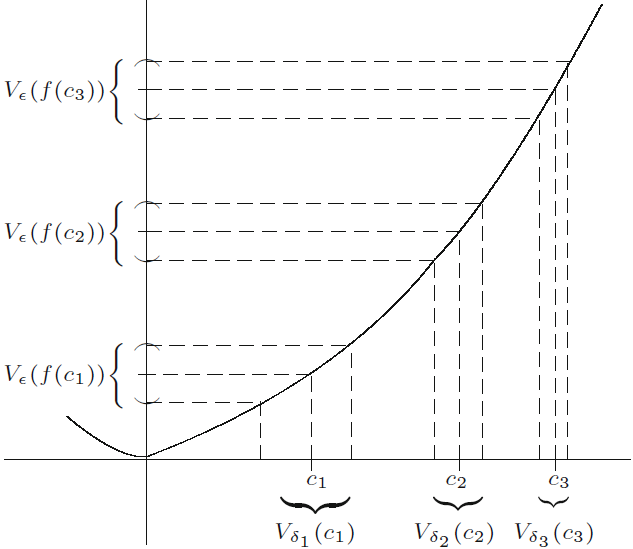
\includegraphics[width=0.7\linewidth]{figs/g(x)=x^2.png}
                \caption{$g(x)=x^2$. A larger $c$ requires a smaller $\delta$.}
                \label{g(x)=x^2}
            \end{figure}
           \\ \\ \fbox{\parbox{\linewidth}{\textbf{Definition 4.4.4 (Uniform Continuity).} A function $f: A \to \mathbb{R}$ is \textit{uniform continuous on $A$} if 
            \begin{equation*}
                \forall \epsilon>0, \exists \delta >0: \forall x,y \in A, |x-y|<\delta \implies |f(x)-f(y)|<\epsilon.
            \end{equation*}}}
            \\ \\
            \textbf{Example:} Prove that $f(x)=x^2$ is uniformly continuous on $[4,8]$.
            \\ \\
            Notice that
            \begin{align*}
                |f(x)-f(y)| = |x^2 - y^2| &= |(x+y)(x-y)| \\
                & = |x+y||x-y| \\
                & \leq (|x|+|y|)|x-y| \\
                & \leq (|8|+|8|)|x-y| \\
                & = 16|x-y|.
            \end{align*}
            Let $\epsilon >0, \delta = \epsilon/16$, then
            \begin{equation*}
                |x-y|<\delta \implies |f(x) - f(y)| \leq 16 |x-y| < (\epsilon/16)16 = \epsilon,
            \end{equation*}
            as desired.
            \\ \\
            \fbox{\parbox{\linewidth}{\textbf{Theorem 4.4.5 (Sequential Criterion for Absence of Uniform Continuity).} \textit{A function $f:A \to \mathbb{R}$ is not uniformly continuous on $A$ iff
            \begin{equation*}
                \exists \epsilon > 0, \exists (x_n),(y_n) \in A: |x_n-y_n| \to 0
            \end{equation*}
            but
            \begin{equation*}
                |f(x_n)-f(y_n)| \geq \epsilon \quad \text{or} \quad \text{ $|f(x)-f(y)|$ does not converge to 0.}
            \end{equation*}
            }}}
            \\ \\
            \textit{*Proof.} $(\Rightarrow)$ Let $f:A \to \mathbb{R}$ be a function that is not uniformly continuous on $A$. Then the negation of Definition 4.4.4 implies that
            \begin{equation*}
                \forall \epsilon > 0, \exists \delta > 0: \forall x,y \in A, |x-y|<\delta \implies |f(x)-f(y)| \geq \epsilon.
            \end{equation*}
            Let $\delta = 1$, then
            \begin{equation*}
                \exists x_1, y_1 \in A: |x_1-y_1|<1 \quad \text{but} \quad |f(x_1)-f(y_1)| \geq \epsilon.
            \end{equation*}
            Let $\delta = 1/2$, then
            \begin{equation*}
                \exists x_2,y_2 \in A: |x_2-y_2| < \frac{1}{2} \quad \text{but} \quad |f(x_2)-f(y_2)| \geq \epsilon.
            \end{equation*}
            In general, let $\delta = 1/n$, then
            \begin{equation*}
                \exists x_n,y_n \in A: |x_n-y_n| < \frac{1}{n} \quad \text{but} \quad |f(x_n)-f(y_n)| \geq \epsilon.
            \end{equation*}
            The resulting sequences $(x_n),(y_n)$ then satisfy
            \begin{equation*}
                |x_n-y_n| \to 0 \quad \text{but} \quad |f(x_n)-f(y_n)| \geq \epsilon,
            \end{equation*}
            as desired.
            \\ \\
            $(\Leftarrow)$ Assume
            \begin{equation*}
                \exists \epsilon > 0, \exists (x_n),(y_n) \in A: |x_n-y_n| \to 0 \quad \text{but} \quad |f(x_n)-f(y_n)| \geq \epsilon.
            \end{equation*}
            For the sake of contradiction, assume that $f: A \to \mathbb{R}$ is uniformly continuous, then by Definition 4.4.4, 
            \begin{equation*}
                \forall \epsilon > 0, \exists \delta > 0: \forall x,y \in A, |x-y|<\delta \implies |f(x)-f(y)| < \epsilon.
            \end{equation*}
            But since $(x_n),(y_n) \in A$, it follows that
            \begin{equation*}
                \exists x\in (x_n),y \in (y_n): |x-y|<\delta \quad \text{but} \quad |f(x)-f(y)| \geq \epsilon.
            \end{equation*}
            This is a contradiction, and hence $f$ is not uniformly continuous. \\ \\
            QED
            \\ \\
            \textbf{Example} (i) Prove that $f(x)=x^2$ is not uniformly continuous on $\mathbb{R}$.
            \\ \\
            WTS: 
            \begin{equation*}
                \exists \epsilon, \exists (x_n),(y_n) \in \mathbb{R}: |x_n-y_n| \to 0 \quad \text{but} \quad |x_n^2-y_n^2| \geq \epsilon.
            \end{equation*}
            Let $x_n = n, y_n = n + (1/n)$ then
            \begin{align*}
                |x_n-y_n| & = |n - (n+(1/n))| \\
                & = |-1/n| \\
                & = 1/n \to 0
            \end{align*}
            but
            \begin{align*}
                \bigg|f(n)-f\bigg(n+\frac{1}{n}\bigg)\bigg| & = \bigg|n^2 - \bigg(n+\frac{1}{n}\bigg)^2\bigg| \\
                & = \bigg|n^2 - \bigg(n^2 + 2 + \frac{1}{n^2}\bigg)\bigg| \\
                & = \bigg|n^2 - n^2 -2 -\frac{1}{n^2}\bigg| \\
                & = \bigg|2+\frac{1}{n^2}\bigg| \\
                & \leq |2| = 2 \geq \epsilon,
            \end{align*}
            as desired.
            \\ \\
            (ii) Let $f = 1/(x-3)$. (a) Find $A$ where $f$ is uniformly continuous. (b) Find $A$ where $f$ is not uniformly continuous.
            \\ \\
            (a) Let $A=[4,8]$. Notice that
            \begin{align*}
                \bigg|\frac{1}{x-3}-\frac{1}{y-3}\bigg| & = \bigg|\frac{y-3-x+3}{(x-3)(y-3)}\bigg| \\
                & = \bigg|\frac{x-y}{(x-3)(y-3)}\bigg| \\
                & = |x-y|\bigg|\frac{1}{x-3}\bigg|\bigg|\frac{1}{y-3}\bigg| \\
                & \leq |x-y|\bigg|\frac{1}{4-3}\bigg|\bigg|\frac{1}{4-3}\bigg| \\
                & = |x-y|.
            \end{align*}
            Let $\epsilon >0, \delta=\epsilon$,
            \begin{equation*}
                |x-y|<\delta \implies \bigg|\frac{1}{x-3}-\frac{1}{y-3}\bigg| \leq |x-y| < \epsilon.
            \end{equation*}
            Hence, $f$ is uniformly continuous on $[4,8]$.
            \\ \\
            (b) Let $A = (3,4]$, and $x_n=3+(1/n), y_n=3+(2/n)$. Then
            \begin{align*}
                |x_n-y_n| &= \bigg|3+\frac{1}{n}-\bigg(3-\frac{2}{n}\bigg)\bigg| \\
                &= \bigg|\frac{-1}{n}\bigg| \\
                & = \frac{1}{n} \to 0.
            \end{align*}
            but
            \begin{align*}
                \bigg|\frac{1}{3+\frac{1}{n}-3} - \frac{1}{3+\frac{2}{n}-3}\bigg| = \bigg|n-\frac{n}{2}\bigg| \geq \frac{1}{2}.
            \end{align*}
            Hence, $f$ is not uniformly continuous on $(3,4]$.
            \\ \\
            \textbf{Example 4.4.6.} The function $h(x)=\sin(1/x)$ (Figure \ref{sin1/x}) is continuous at every point in $(0,1)$ but is not continuous in $(0,1)$. 
            \\ \\
            Let
            \begin{equation*}
                x_n=\frac{1}{\frac{\pi}{2}+2n\pi} \quad \text{and} \quad y_n = \frac{1}{\frac{3\pi}{2}+2n\pi}.
            \end{equation*}
            Then
            \begin{align*}
                |x_n-y_n| & = \bigg|\frac{1}{\frac{\pi}{2}+2n\pi} - \frac{1}{\frac{3\pi}{2}+2n\pi}\bigg| \\
                & = \bigg|\frac{\frac{3\pi}{2}+2n\pi - \frac{\pi}{2}-2n\pi}{(\frac{\pi}{2}+2n\pi)(\frac{3\pi}{2}+2n\pi)}\bigg| \\
                &= \bigg|\frac{\pi}{(\frac{\pi}{2}+2n\pi)(\frac{3\pi}{2}+2n\pi)}\bigg| \\
                & = \pi \bigg|\frac{1}{\frac{\pi}{2}+2n\pi}\bigg|\bigg|\frac{1}{\frac{3\pi}{2}+2n\pi}\bigg| \to 0.
            \end{align*}
            but
            \begin{equation*}
                |\sin(\frac{\pi}{2}+2n\pi) - \sin(\frac{3\pi}{2}+2n\pi) = |1-(-1)| = 2,
            \end{equation*}
            as desired.
            \\ \\
            \fbox{\parbox{\linewidth}{\textbf{Theorem 4.4.7 (Uniform Continuity on Compact Sets.).} \textit{A function that is continuous on a compact set $K$ is uniformly continuous on $K$.}}}
            \\ \\
            \textit{Proof.} Let $f$ be a function that is continuous on a compact set $K$.
            \\ \\
            For the sake of contradiction, assume that $f$ is not uniformly continuous on $K$. Then
            \begin{equation*}
                \exists \epsilon>0, \exists (x_n),(y_n) \in K: |x_n-y_n|\to0 \quad \text{but} \quad |f(x_n)-f(y_n)|\geq \epsilon.
            \end{equation*}
            Since $K$ is compact, and $(x_n),(y_n)\in K$, $(x_n),(y_n)$ must contain subsequences
            \begin{equation*}
                (x_{n_k}) \to x \in K \quad \text{and} \quad (y_{n_k}) \to y \in K.
            \end{equation*}
            Since $x,y \in K$ and $f$ is continuous on $K$,
            \begin{align*}
                (x_{n_k}) \to x \implies f(x_{n_k}) \to f(x) \quad \text{and} \quad 
                (y_{n_k}) \to y \implies f(y_{n_k}) \to f(y).
            \end{align*}
            Since $|x_n-y_n|\to0$, the terms $x_n,y_n$ are getting closer to each other and hence must converge to the same value. Therefore $x=y$ and
            \begin{equation*}
                |f(x_{n_k})-f(_{n_k})| \to |f(x)-f(y)| = 0 < \epsilon,
            \end{equation*}
            a contradiction. Hence, $f$ is uniformly continuous on $K$.
            \\ \\
            QED
            
            \subsection{The Intermediate Value Theorem}
            \fbox{\parbox{\linewidth}{\textbf{Theorem 4.5.1 (Intermediate Value Theorem).} \textit{Let $f: [a,b] \to \mathbb{R}$ be continuous.}
            \begin{equation*}
                L \in \mathbb{R}: f(a) < L < f(b) \quad \text{or} \quad f(a)>L>f(b) \implies \exists c \in (a,b): f(c)=L
            \end{equation*}}}
            
            \begin{figure}[ht!]
                \centering
                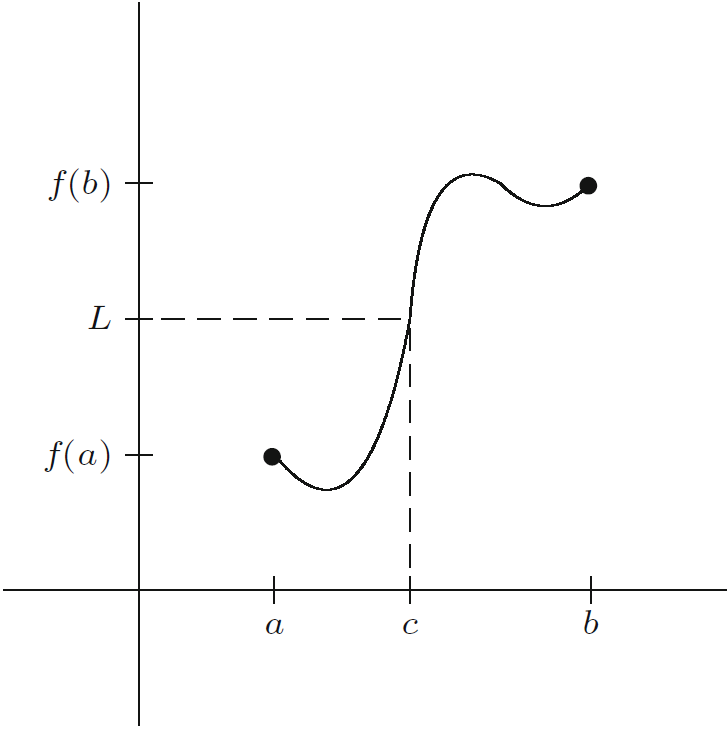
\includegraphics[width=0.55\linewidth]{figs/IVT.png}
                \caption{The Intermediate Value Theorem.}
                \label{ivt}
            \end{figure}
            
            \subsubsection{Preservation of Connected Sets}
            \fbox{\parbox{\linewidth}{\textbf{Theorem 4.5.2 (Preservation of Connected Sets).} \textit{Let $f: G \to \mathbb{R}$ be continuous.
            \begin{equation*}
                E \subseteq G \text{ is connected} \implies f(E) \text{ is connected.}
            \end{equation*}}}}
            \\ \\
            \textit{Proof.} Let $f:G \to \mathbb{R}$ be continuous, and $E \subseteq G$ is a connected.
            \\ \\
            For the sake of contradiction, assume $f(E)$ is not connected. So $f(E) = A \cup B$,
            \begin{equation*}
                \overline{A} \cap B = \emptyset \quad \text{and} \quad A \cap \overline{B} = \emptyset.
            \end{equation*}
            Let 
            \begin{equation*}
                C = f^{-1}(A) \cap E = \{x \in G: f(x) \in A\} \quad \text{and} \quad D = f^{-1}(B) \cap E = \{x \in G: f(x) \in B\}.
            \end{equation*}
            Since $f(E) = A \cup B$, it follows that $E = C \cup D$. Because $E$ is connected, 
            \begin{equation*}
                \overline{C} \cap D \neq \emptyset \quad \text{and} \quad C \cap \overline{D} \neq \emptyset.
            \end{equation*}
            So $\exists x \in G: x \in \overline{C} \cap D$. It follows that $x \in \overline{C}$ and $x \in D$. If $x \in D$, then $f(x) \in B$. Because $f$ is continuous, if $x \in \overline{C}$, then $f(x)$ is a limit point of $A$ and $f(x) \in \overline{A}$. Since $f(x) \in \overline{A}$ and $f(x) \in B$, it follows that $f(x) \in \overline{A} \cap B$ and $\overline{A} \cap B \neq \emptyset$. This contradicts that $f(E)=A \cap B$ is disconnected. Therefore, $f(E)$ is connected.
            \\ \\
            QED
            \\ \\
            \textbf{Example.} (i) Show that $\exists c \in \mathbb{R}: c^2=2$.
            \\ \\
            Let $f(x) = x^2 - 2$, then $f(0) = -2$ and $f(2) = 2$. So $f(0)<0<f(2)$. By the Intermediate Value Theorem,
            $\exists c \in \mathbb{R}: 0 <c<2$ and $f(c) = c^2 - 2 = 0 \implies c^2 = 2$, as desired.
            \\ \\
            (ii) Show that $\exists c \in \mathbb{R}: e^c = 2$.
            \\ \\
            Let $f(x) = e^x -2$, then $f(0)=-2$ and $f(1)=e-2>0$. So $f(0)<0<f(1)$. By the Intermediate Value Theorem, $\exists c \in \mathbb{R}: 0 < c < 1$ and $f(c) = e^c -2 =0 \implies e^c = 2$, as desired.
            
            \section{The Derivative}
            \subsection{Discussion: Are Derivatives Continuous?}
            
            \subsection{Derivatives and the Intermediate Value Property}
            \fbox{\parbox{\linewidth}{\textbf{Definition 5.2.1 (Differentiability).} Let $f:A \to \mathbb{R}$ be a function defined on $A$ Given $c\in A$, the \textit{derivative of $f$ at $c$} is defined by
            \begin{equation*}
                f'(c) = \lim_{x\to c}\frac{f(x)-f(c)}{x-c},
            \end{equation*}
            provided this limit exists. In this case $f$ \textit{is differentiable at} $c$. If $f'$ exists for $\forall c \in A$, then $f$ \textit{is differentiable on $A$}.}}
            \\ \\
            \textbf{Example 5.2.2.} (i) Let $f(x)=x^n, n \in \mathbb{N}$, and $c \in \mathbb{R}$ be arbitrary. Using the algebraic identity
            \begin{equation*}
                x^n-c^n = (x-c)(x^{n-1}+cx^{n-2}+c^2x^{n-3}+\dots+c^{n-1}),
            \end{equation*}
            the derivative of $f$ at $c$ is
            \begin{align*}
                f'(c) = \lim_{x\to c} \frac{x^n - c^n}{x-c} & = \lim_{x \to c} \frac{(x-c)(x^{n-1}+cx^{n-2}+c^2x^{n-3}+\dots+c^{n-1})}{x-c} \\
                & = \lim_{x \to c} x^{n-1}+cx^{n-2}+c^2x^{n-3}+\dots+c^{n-1} \\
                & = c^{n-1}+c\cdot c^{n-2}+c^2\cdot c^{n-3} + \dots c^{n-1} \\
                & = c^{n-1}+c^{n-1}+\dots+c^{n-1} \\
                & = nc^{n-1}.
            \end{align*}
            (ii) Let $f(x) = |x|$. The derivative of $f$ at $c=0$ is
            \begin{align*}
                f'(0) = \lim_{x \to 0} \frac{|x|}{x}.
            \end{align*}
            Let $g(x)=|x|/x$ and $x_n=1/n,y_n=-1/n$, it follows that
            \begin{equation*}
                (x_n) \to 0, (y_n) \to 0 \quad \text{but} \quad g(x_n) = \frac{|1/n|}{1/n} = 1, g(y_n) = \frac{|-1/n|}{-1/n} = -1.
            \end{equation*}
            So the limit $\lim_{x \to 0}|x|/x$ does not exist and hence $f$ is not differentiable at 0.
            \\ \\
            Example 5.2.2 (ii) shows that $f$ is continuous does not mean that $f$ is differentiable.
            \\ \\
            \fbox{\parbox{\linewidth}{\textbf{Theorem 5.2.3.} \textit{If $g:A \to \mathbb{R}$ is differentiable at $c \in A$, then $f$ is continuous at $c$.}}}
            \\ \\
            \textit{Proof.} Assume $f$ is differentiable at $c$. So
            \begin{equation*}
                f'(c) = \lim_{x \to c} \frac{f(x)-f(c)}{x-c}
            \end{equation*}
            exists, then
            \begin{align*}
                \lim_{x \to c} (f(x)-f(c)) &= \lim_{x \to c} \bigg(\frac{f(x)-f(c)}{x-c}\bigg)(x-c) \\
                & = \lim_{x \to c} \frac{f(x)-f(c)}{x-c} \lim_{x \to c}(x-c) \\
                & = f'(c) \cdot 0 \\
                & = 0.
            \end{align*}
            It follows that
            \begin{equation*}
                \lim_{x \to c} (f(x)-f(c)) = \lim_{x-c} f(x) - \lim_{x-c}f(c) = \lim_{x-c} f(x) - f(c) = 0 \implies \lim_{x \to c} f(x) = f(c).
            \end{equation*}
            Therefore, $f$ is continuous at $c$.
            \\ \\
            QED
            
            \subsubsection{Combinations of Differentiable Functions}
            \fbox{\parbox{\linewidth}{\textbf{Theorem 5.2.4 (Algebraic Differentiability Theorem).} \textit{Let $f$ and $g$ be functions defined on an interval $A$, and assume both are differentiable at $c \in A$. Then,}
            \begin{enumerate}[label=(\roman*)]
                \item $(f+g)'(c) = f'(c)+g'(c)$,
                \item $(kf)'(c) = kf'(c), \forall k \in \mathbb{R}$,
                \item $(fg)'(c) = f'(c)g(c) + f(c)g'(c)$,
                \item $(f/g)'(c) = \frac{g(c)f'(c)-f(c)g'(c)}{(g(c))^2}, g(c) \neq 0.$
            \end{enumerate}
            }}
            \\ \\
            \textit{Proof.} (i) 
            \\ \\
            (ii)
            \\ \\
            (iii) By Definition 5.2.1.,
            \begin{align*}
                (fg)'(c) &= \lim_{x \to c} \frac{f(x)g(x)-f(c)g(c)}{x-c} \\
                & = \lim_{x \to c} \frac{f(x)g(x) + f(x)g(c) - f(x)g(c) - f(c)g(c)}{x-c} \\
                & = \lim_{x \to c} \frac{(f(x)g(x) - f(x)g(c)) + (f(x)g(c) - f(c)g(c))}{x-c} \\
                & = \lim_{x \to c} \bigg(\frac{f(x)g(x)-f(x)g(c)}{x-c}+\frac{f(x)g(c)-f(c)g(c)}{x-c}\bigg) \\
                & = \lim_{x \to c}f(x)\frac{g(x)-g(c)}{x-c}+\lim_{x \to c}g(c)\frac{f(x)-f(c)}{x-c} \\
                & = \lim_{x \to c}f(x) \lim_{x \to c}\frac{g(x)-g(c)}{x-c} + g(c)\lim_{x \to c}\frac{f(x)-f(c)}{x-c} \\
                & = f(c)g'(c) + g(c)f'(c).
            \end{align*}
            \\ \\
            (iv)
            \\ \\
            QED
            \\ \\
            \fbox{\parbox{\linewidth}{\textbf{Theorem 5.2.5 (Chain Rule).} \textit{Let $f:A \to \mathbb{R}$ and $g: B \to \mathbb{R}$ satisfy $f(A) \subseteq B$ so that $g \circ f$ is defined. If $f$ is differentiable at $c \in A$ and if $g$ is differentiable at $f(c) \in B$, then $g \circ f$ if differentiable at $c$ with $(g \circ f)'(c)=g'(f(c))\cdot f'(c)$.}}}
            \\ \\
            \textit{Proof.} By Definition 5.2.1, 
            \begin{equation*}
                g'(f(c)) = \lim_{y \to f(c)}\frac{g(y)-g(f(c))}{y-f(c)}.
            \end{equation*}
            Let $d(y)$ be the difference quotient
            \begin{equation}
                d(y) = \frac{g(y)-g(f(c))}{y-f(c)},
            \label{diff_quot}
            \end{equation}
            and 
            \begin{equation*}
                \lim_{y \to f(c)} d(y) = \lim_{y \to f(c)} \frac{g(y)-g(f(c))}{y-f(c)} = g'(f(c)).
            \end{equation*}
            Write $d(f(c)) = g'(f(c))$ so that $d$ is continuous at $f(c)$.
            \\ \\
            Equation (\ref{diff_quot}) can be rewritten as
            \begin{equation}
                g(y)-g(f(c)) = d(y)(y-f(c)).
            \end{equation}
            Let $y = f(x)$ and divide both sides by $x-c$,
            \begin{align*}
                \frac{g(f(x))-g(f(c))}{x-c} & = d(f(x)) \frac{f(x)-f(c)}{x-c} \\
                \lim_{x \to c} \frac{g(f(x))-g(f(c))}{x-c} & = \lim_{x \to c} d(f(x)) \frac{f(x)-f(c)}{x-c} \\
                (g \circ f)'(c) & = \lim_{x \to c} d(f(x)) \lim_{x \to c} \frac{f(x)-f(c)}{x-c} \\
                & = g'(f(c))  f'(c).
            \end{align*}
            \\ \\
            QED
            
            \subsubsection{Darboux's Theorem}
            \fbox{\parbox{\linewidth}{\textbf{Theorem 5.2.6 (Interior Extremum Theorem).} \textit{Let $f$ be differentiable on $(a,b)$. If $f$ attains a maximum or minimum value at $c\in (a,b)$, then $f'(c)=0$.}}}
            \\ \\
            \textit{Proof.} Let $f(c)$ be a maximum, and let $(x_n), (y_n)$ be two sequences that converges to $c$ where $x_n < c < y_n, \forall n \in \mathbb{N}$. Since $f(c)$ is a maximum, it follows that $f(x_n) - f(c) \leq 0, \forall n \in \mathbb{N}$ and $x_n - c < 0$. So
            \begin{equation*}
                f'(c) = \lim_{n \to \infty}\frac{f(x_n)-f(c)}{x_n-c} \geq 0.
            \end{equation*}
            Similarly, $f(y_n) - f(c) \leq 0, \forall n \in \mathbb{N}$ and $y_n - c > 0$, so
            \begin{equation*}
                f'(c) = \lim_{n \to \infty}\frac{f(x_n)-f(c)}{x_n-c} \leq 0.
            \end{equation*}
            Since $f'(c) \geq 0$ and $f'(c) \leq 0$, it follows that $f'(c) = 0$.
            \\ \\
            QED
            \\ \\
            \begin{figure}[ht!]
                \centering
                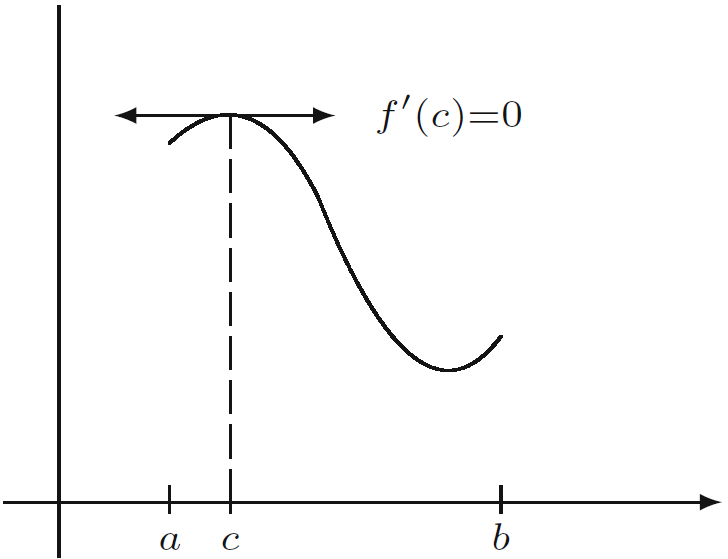
\includegraphics[width=0.5\linewidth]{figs/interior_extremum.png}
                \caption{The Interior Extremum Theorem.}
                \label{fig:my_label}
            \end{figure}
            \fbox{\parbox{\linewidth}{\textbf{*Theorem 5.2.7 (Darboux's Theorem).} \textit{If $f$ is differentiable on $[a,b]$, and if $\alpha$ satisfies $f'(a) < \alpha < f'(b)$ or $f'(a) > \alpha > f'(b)$, then $\exists c \in (a,b): f'(c) = \alpha$.}}}
            
            \subsection{The Mean Value Theorems}
            \fbox{\parbox{\linewidth}{\textbf{Theorem 5.3.1 (Rolle's Theorem).} \textit{Let $f: [a,b] \to \mathbb{R}$ be continuous on $[a,b]$ and differentiable on $(a,b)$, then
            \begin{equation*}
                f(a) = f(b) \implies \exists c \in (a,b): f'(c)=0.
            \end{equation*}
            }}}
            \\ \\
            \textit{Proof.} Since $f$ is continuous on $[a,b]$ and $[a,b]$ is compact, by the Extreme Value Theorem (Theorem 4.4.2.), $f$ attains a maximum and minimum value on $[a,b]$. Since $f(a)=f(b)$, if both the maximum and minimum occur at the endpoints, $f$ must be a constant function and $f'(x)=0, \forall x \in (a,b)$. If the maximum and minimum do not occur on the endpoints, then $\exists c \in (a,b)$ such that $f(c)$ is the maximum or minimum. Since $f$ is differentiable on $(a,b)$, by the Interior Extremum Theorem (Theorem 5.2.6.), $f'(c)=0$.
            \\ \\
            QED
            \\ \\
            \begin{figure}[ht!]
                \centering
                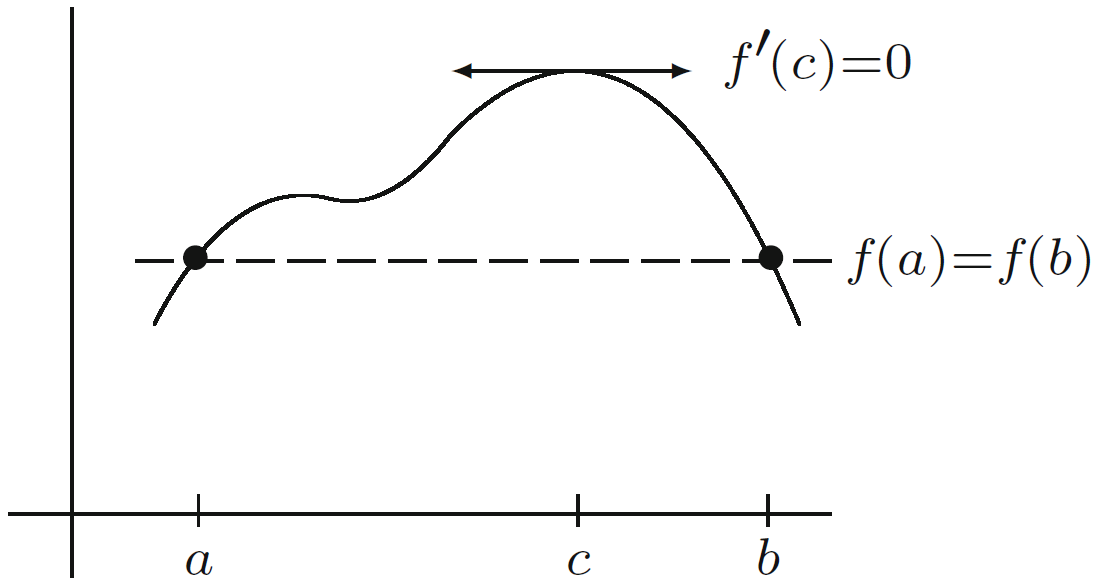
\includegraphics[width=0.6\linewidth]{figs/rolles_thm.png}
                \caption{Rolle's Theorem.}
                \label{rolles_thm}
            \end{figure}
            \fbox{\parbox{\linewidth}{\textbf{Theorem 5.3.2 (Mean Value Theorem).} \textit{If $f: [a,b] \to \mathbb{R}$ is continuous on $[a,b]$ and differentiable on $(a,b)$, then
            \begin{equation*}
                \exists c \in (a,b): f'(c) = \frac{f(b)-f(a)}{b-a}.
            \end{equation*}
            }}}
            \\ \\
        \textit{Proof.} The Mean Value Theorem reduces to Rolle's Theorem in the case where $f(a)=f(b)$. The strategy of the proof is to reduce the more general statement to this special case.
        \\ \\
        The equation of the line through $(a,f(a))$ and $(b,f(b))$ is
        \begin{equation*}
            y = \bigg(\frac{f(b)-f(a)}{b-a}(x-a)+f(a)\bigg).
        \end{equation*}
        \begin{figure}[ht!]
            \centering
            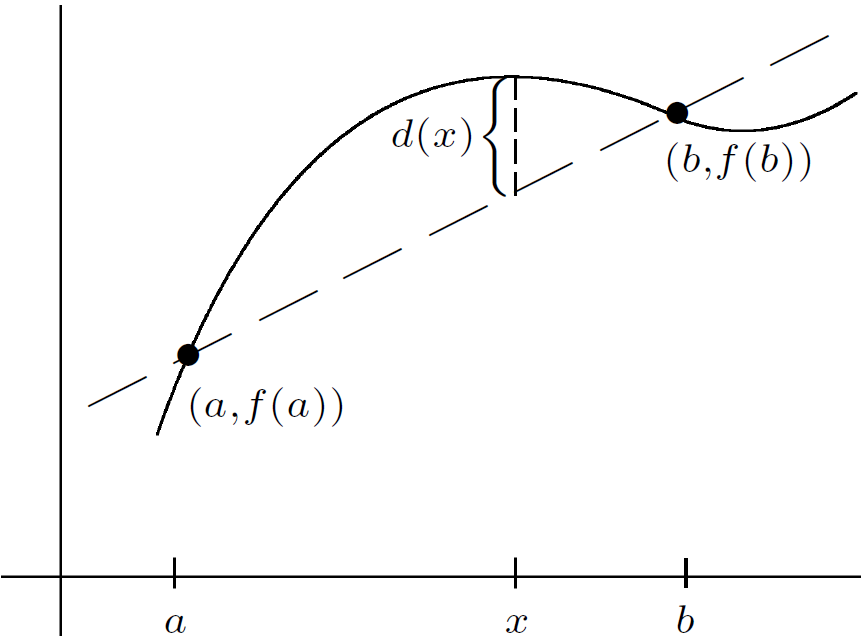
\includegraphics[width=0.5\linewidth]{figs/d(x).png}
        \end{figure}
        Let 
        \begin{equation*}
            d(x) = f(x) - \bigg[\bigg(\frac{f(b)-f(a)}{b-a}(x-a)+f(a)\bigg)\bigg],
        \end{equation*}
        since
        \begin{align*}
            d(a) &= f(a) - \bigg[\bigg(\frac{f(b)-f(a)}{b-a}(a-a)+f(a)\bigg)\bigg] = 0 \\
            d(b) &= f(a) - \bigg[\bigg(\frac{f(b)-f(a)}{b-a}(b-a)+f(a)\bigg)\bigg] = 0,
        \end{align*}
        it follows that $d(a) = d(b) = 0$. So $d(x)$ is just $f(x)$ rotated such that $f(a),f(b)$ are on the $x$-axis. This implies that $d(x)$ is continuous on $[a,b]$ and differentiable on $(a,b)$. So by the Rolle's Theorem, $\exists c \in (a,b): d'(c)=0$. Notice that
        \begin{align*}
            d'(x) &= f'(x) - \bigg[\bigg(\frac{f(b)-f(a)}{b-a}(1)+0\bigg)\bigg] \\
            &= f'(x) - \bigg(\frac{f(b)-f(a)}{b-a}\bigg).
        \end{align*}
        So
        \begin{align*}
            d'(c) = 0 = f'(c) - \bigg(\frac{f(b)-f(a)}{b-a}\bigg) \implies 
            f'(c) = \frac{f(b)-f(a)}{b-a}.
        \end{align*}
        \\ \\
        QED
        \\ \\
        \fbox{\parbox{\linewidth}{\textbf{Corollary 5.3.3.} \textit{If $g:A \to \mathbb{R}$ is differentiable on an interval $A$ and satisfies $g'(x)=0, \forall x \in A$, then $g(x)=k$ for some constant $k \in \mathbb{R}$.}}}
            \\ \\
            \textit{Proof.} Let $x,y \in A$ be arbitray and assume $x<y$. By the Mean Value Theorem,
            \begin{equation*}
                g'(c) = \frac{g(y)-g(x)}{y-x}, \exists c \in A.
            \end{equation*}
            Since $g'(c)=0$, it follows that $g(y)=g(x)=k, \forall x \in A$.
            \\ \\
            QED
            \\ \\
            \fbox{\parbox{\linewidth}{\textbf{Corollary 5.3.4.} \textit{If $f$ and $g$ are differentiable on A and $f'(x)=g'(x), \forall x \in A$, then $f(x)=g(x)+k, \exists k \in \mathbb{R}$.}}}
            \\ \\
            \textit{Proof.} Let $h(x) = f(x) - g(x)$. Since $f'(x)=g'(x)$, it follows that
            \begin{equation*}
                h'(x) = f'(x) - g'(x) = 0, \forall x \in A.
            \end{equation*}
            Since $h(x)$ is differentiable on $A$ and $h'(x)=0, \forall x \in A$, by Corollary 5.3.3, $h(x)=k$ for some constant $k \in \mathbb{R}$ and hence
            \begin{equation*}
                k = f(x) - g(x) \implies f(x) = g(x) + k.
            \end{equation*}
            QED
            
            \section{Sequences and Series of Functions}
            \subsection{Discussion: The Power of Power Series}
            \subsection{Uniform Convegence of a Sequence of Functions}
           \subsubsection{Pointwise Convergence} \fbox{\parbox{\linewidth}{\textbf{Definition 6.2.1.} Let $f_n, \forall n \in \mathbb{N}$ be defined on $A \subseteq \mathbb{R}$. The sequence of functions $(f_n)$ \textit{converges pointwise on} $A$ to a function $f$ if $\lim_{n \to \infty} f_n(x) = f(x),\forall x \in A$.}}
           \\ \\
           \textbf{Example.} (i) Let $f_n(x) = \sin(x/n)$, then
           \begin{align*}
               \lim_{n \to \infty} \sin(x/n) = \sin(0) = 0, \forall x \in \mathbb{R}.
           \end{align*}
           Hence $f_n(x) = \sin(x/n)$ converges pointwise to $\sin(0)$.
           \\ \\
           (ii) Let $f_n(x) = e^{nx}$. 
           If $x < 0$, then
           \begin{align*}
               \lim_{n \to \infty} e^{nx} = \lim_{n \to \infty} (e^x)^n  = 0, \forall x \in (-\infty,0]
           \end{align*}
           since $e^x<1$. If $x=0$, then
           \begin{align*}
               \lim_{n \to \infty} e^{0}  = 1.
           \end{align*}
           If $x>0$, then $\lim_{n \to \infty} e^{nx}$ diverges. Hence, the sequence of functions diverges when $x>0$ and
           \begin{equation*}
               \lim_{n \to \infty} e^{nx} = \bigg\{ \begin{matrix} 0 & ,x < 0 \\ 1 & ,x=0. \end{matrix}
           \end{equation*}
           \\
           \textbf{Example 6.2.2.} (i) Let $f_n(x) = (x^2+nx)/n$ on all of $\mathbb{R}$. Fig. \ref{6.2.2(i)} shows what happens when $n$ gets larger. Algebraically,
           \begin{align*}
               \lim_{n \to \infty} \frac{x^2+nx}{n} = \lim_{n \to \infty} \frac{x^2}{n} + x = x.
           \end{align*}
           Thus, $(f_n)$ converges pointwise to $f(x)=x$ on $\mathbb{R}$.
           \\ \\
           (ii) Let $g_n(x) = x^n$ on $[0,1]$. Fig. \ref{6.2.2(ii)} shows what happens when $n \to \infty$. If $0 \leq x < 1$, then $x^n \to 0$. If $x=1$, then $x^n \to 1$. Thus,
           \begin{equation*}
               \lim_{n \to \infty} g_n(x) = \bigg\{ \begin{matrix} 0 &, x \in [0,1) \\
               1 &, x=1. \end{matrix}
           \end{equation*}
           \\ \\
           (iii) Let $h_n(x) = x^{1 + \frac{1}{2n-1}}$ on $[-1,1]$ (Fig. \ref{6.2.2(iii)}). Then,
           \begin{equation*}
               \lim_{n \to \infty} x^{1 + \frac{1}{2n-1}} = x \lim_{n \to \infty} x^{\frac{1}{2n-1}} = |x|, \forall x \in [-1,1].
           \end{equation*}
           Hence, $\lim_{n \to \infty} h_n(x) = f(x)=|x|$ on $[-1,1]$.
           \\ \\
           In Example 6.2.2 (ii), the sequence of continuous functions converges to a function that is not continuous. In Example 6.2.2 (iii), the sequence of differentiable functions converges to a function that is not differentiable at $x=0$.
           
           \begin{figure}[ht!]
               \centering
               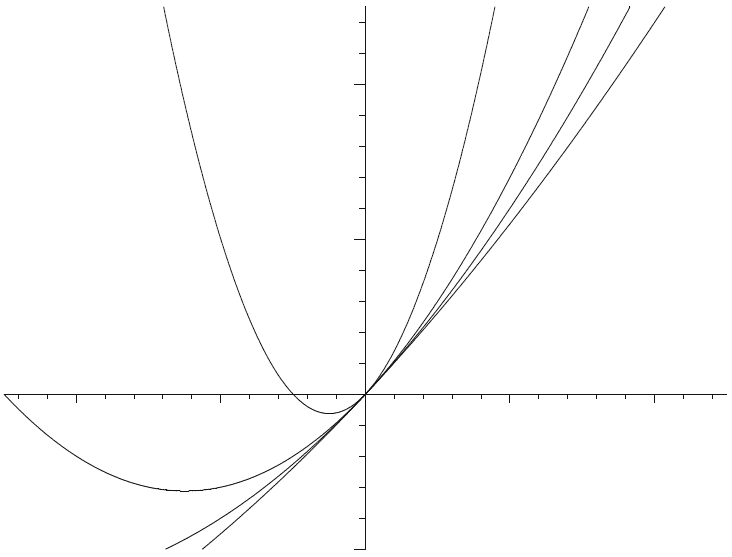
\includegraphics[width=0.6\linewidth]{figs/exp6.2.2(i).png}
               \caption{$f_1,f_5,f_{10}$ and $f_{20}$ where $f_n(x) = (x^2+nx)/n$.}
               \label{6.2.2(i)}
           \end{figure}
           
           \begin{figure}[ht!]
               \centering
               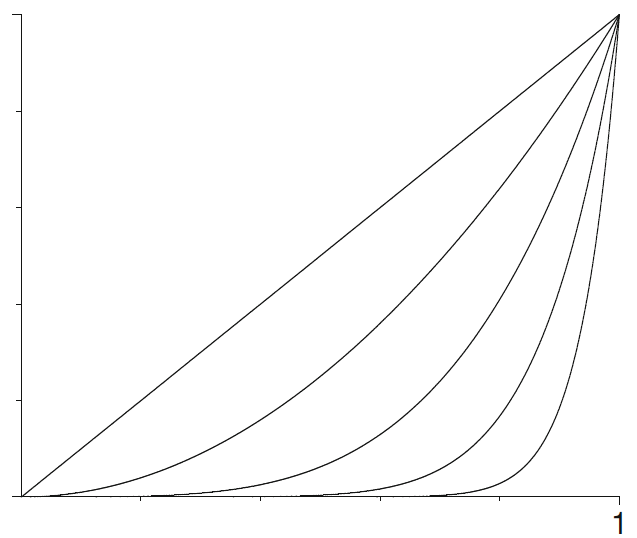
\includegraphics[width=0.6\linewidth]{figs/exp6.2.2(ii).png}
               \caption{$g(x)=\lim_{n \to \infty} x^n$ is not continuous on $[0,1]$.}
               \label{6.2.2(ii)}
           \end{figure}
           
           \begin{figure}[ht!]
               \centering
               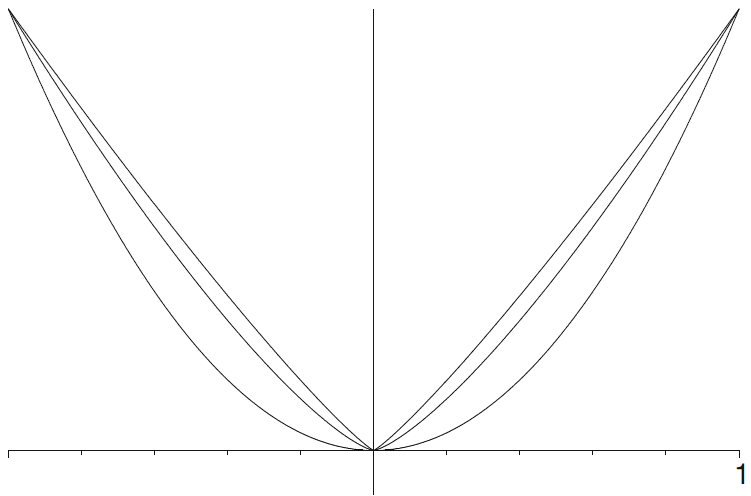
\includegraphics[width=0.6\linewidth]{figs/exp6.2.2(iii).png}
               \caption{$h_n \to |x|$ on $[-1,1]$. The function $f(x)=|x|$ is not differentiable at $x=0$.}
               \label{6.2.2(iii)}
           \end{figure}
           
           \subsubsection{Uniform Convergence}
           \fbox{\parbox{\linewidth}{\textbf{Definition 6.2.3 (Uniform Convergence).} Let $(f_n)$ be a sequence of functions defined on $A \subseteq \mathbb{R}$. Then, $(f_n)$ \textit{converges uniformly on} $A$ to a limit function $f$ defined on $A$ if
           \begin{equation*}
               \forall \epsilon > 0, \exists N \in \mathbb{N}: n \geq N \implies |f_n(x)-f(x)| < \epsilon, \forall x \in A.
           \end{equation*}
           }}
           \\ \\
           \fbox{\parbox{\linewidth}{\textbf{Definition 6.2.1B.} Let $(f_n)$ be a sequence of functions defined on $A \subseteq \mathbb{R}$. Then $(f_n)$ \textit{converges pointwise on} $A$ to a limit function $f$ defined on $A$ if
           \begin{equation*}
               \forall \epsilon > 0, \exists N \in \mathbb{N} \text{ (perhaps depends on $x$)}: n \geq N \implies |f_n(x) - f(x)| < \epsilon.
           \end{equation*}
           }}
           \\ \\
           The difference between uniform convergence and pointwise convergence is that the same $N$ works for all $x$ for uniform convergence, while different $N$ might be required for different $x$ for pointwise convergence.
           
           \begin{figure}[ht!]
               \centering
               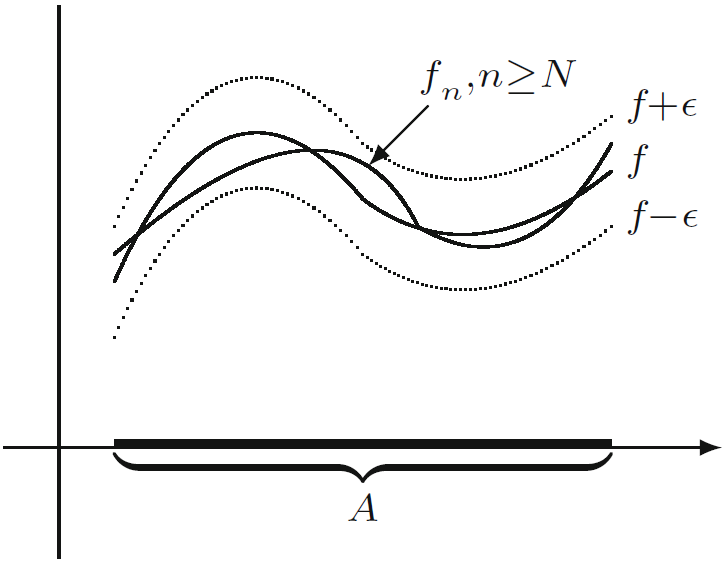
\includegraphics[width=0.5\linewidth]{figs/uniform_cont.png}
               \caption{$f_n \to f$ uniformly on $A$.}
               \label{uniform_cont}
           \end{figure}
           
           \begin{figure}[ht!]
               \centering
               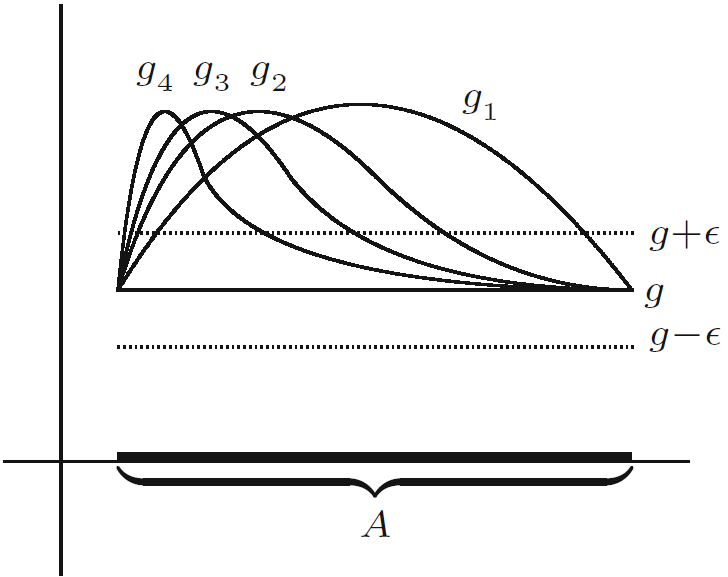
\includegraphics[width=0.5\linewidth]{figs/pointwise_cont.png}
               \caption{$g_n \to g$ pointwise but not uniformly.}
               \label{pointwise_cont}
           \end{figure}
           
           \textbf{Example.} (i) Show that $f_n(x) = 1/nx$ converges uniformly to $f(x) = 0$ on $[1,\infty)$. Notice that 
           \begin{equation*}
               \bigg|\frac{1}{nx} - 0\bigg| = \bigg|\frac{1}{nx}\bigg|
               = \frac{1}{nx}
               \leq \frac{1}{n}.
           \end{equation*}
           Let $\epsilon > 0, N > 1/\epsilon$, 
           \begin{equation*}
               n \geq N \implies \bigg|\frac{1}{nx} - 0\bigg| \leq \frac{1}{n} \leq \frac{1}{N} < \frac{1}{1/\epsilon} = \epsilon,
           \end{equation*}
           as desired.
           \\ \\
           (ii) Let $f_n(x)=x^2/n$. Since
           \begin{equation*}
               \lim_{n \to \infty} \frac{x^2}{n} = 0, \forall x \in \mathbb{R},
           \end{equation*}
           the sequence of functions $x^2/n \to f(x)=0$ pointwise. If $x^2/n \to f(x)=0$ uniformly, then
           \begin{equation*}
               \forall \epsilon > 0, \exists N \in \mathbb{N}: n \geq N \implies  \bigg|\frac{x^2}{n} - 0\bigg| < \epsilon, \forall x \in \mathbb{R}.
           \end{equation*}
           But $|(x^2/n)-0|<\epsilon$ is not true for all $x \in \mathbb{R}$. For any fixed $n$, there exists some $x$ so large that $x^2/n > \epsilon$. So there exists no $N$ for which 
           \begin{equation*}
               n \geq N \implies x^2/n \in V_\epsilon(0), \forall x \in \mathbb{R}.
           \end{equation*}
           To be specific, notice that
           \begin{align*}
               \bigg|\frac{x^2}{n}-0\bigg| = \bigg|\frac{x^2}{n}\bigg| = \frac{x^2}{n}.
           \end{align*}
           Let $\epsilon >0, N > x^2/\epsilon$, this $N$ is dependent on $x$ and cannot work for all $x$. Hence $x^2/n$ does not converge to $f(x)=0$ uniformly.
           \\ \\
           (iii) Let $f_n(x) = e^{nx}$. The sequence of functions $e^{nx} \to f(x)$ pointwise, where
           \begin{equation*}
               f(x) = \bigg\{ \begin{matrix} 0 & ,x<0 \\ 1 & ,x =0\end{matrix}.
           \end{equation*}
           Since for any fixed $n$, there exists some $x$ so large such that $e^{nx} > \epsilon$, it follows that $e^{nx}$ does not converge to $f(x)=0$ uniformly.
           \\ \\
           (iv) Let $f_n(x) = \cos(x/n)$. Since
           \begin{equation*}
               \lim_{n \to \infty} \cos(x/n) = \cos(0) = 1, \forall x \in \mathbb{R},
           \end{equation*}
           $\cos(x/n) \to f(x)=1$ pointwise. But for any fixed $n$, there exists some $x$ such that $\cos(x/n)=-1$ and 
           \begin{equation*}
               |\cos(x/n)-1| = |-1-1| = 2 > \epsilon.
           \end{equation*}
           Hence $\cos(x/n)$ does not converge to $f(x)=1$ uniformly.
           \\ \\
           \textbf{Example 6.2.4.} (i) Let
           \begin{equation*}
               g_n(x) = \frac{1}{n(1+x^2)}.
           \end{equation*}
           Since for any fixed $x \in \mathbb{R}$, $\lim_{n \to \infty} g_n(x) = 0$, the sequence of functions converges ponintwise to $g(x)=0$ on $\mathbb{R}$. Notice that
           \begin{equation*}
               \bigg|\frac{1}{n(1+x^2)} - 0\bigg| = \bigg|\frac{1}{n}\bigg| \bigg|\frac{1}{1+x^2}\bigg| \leq \frac{1}{n}.
           \end{equation*}
           Let $\epsilon > 0, N = 1/\epsilon$,
           \begin{equation*}
               n > N \implies \bigg|\frac{1}{n(1+x^2)} - 0\bigg| \leq \frac{1}{n} < \frac{1}{N} = \frac{1}{1/\epsilon} = \epsilon.
           \end{equation*}
           Hence, $g_n(x)$ converges uniformly to $g(x)=0$ on $\mathbb{R}$.
           \\ \\
           (ii) In Example 6.2.2 (i), $f_n(x) = (x^2+nx)/n$ converges pointwise to $f(x)=x$ on $\mathbb{R}$. On $\mathbb{R}$, the convergence is not uniform. Notice that
           \begin{equation*}
               \bigg|\frac{x^2+nx}{n} - x\bigg| = \frac{x^2}{n}.
           \end{equation*}
           So it must be that $N > x^2/\epsilon$. Since there is no way to choose a single $N$ that works for all $x$ at the same time, the convergence is not uniform.
           
           \subsubsection{Continuity Revisited}
           \fbox{\parbox{\linewidth}{\textbf{Theorem 6.2.6 (Continuous Limit Theorem)}. \textit{Let $(f_n)$ be a sequence of functions defined on $A \subseteq \mathbb{R}$ that converges uniformly on $A$ to a function $f$. If each $f_n$ is continuous at $c \in A$, then $f$ is continuous at $c$.}}}
           \\ \\
           \textit{Proof.} Let each $f_n$ be continuous at $ c \in A$ and let $\epsilon >0$.
           \\ \\
           WTS: $\forall \epsilon >0, \exists \delta>0: 0<|x-c|<\delta \implies |f(x)-f(x)|<\epsilon.$
           \\ \\
           Since $f_n \to f$ uniformly,
           \begin{equation*}
               \exists N \in \mathbb{N}: n \geq N \implies |f_n(x) - f(x)| < \frac{\epsilon}{3} \quad \text{and} \quad |f_n(c)-f(c)| < \frac{\epsilon}{3}.
           \end{equation*}
           Since $f_N$ is continuous at $c \in A$,
           \begin{equation*}
               \exists \delta > 0: |x-c| < \delta \implies |f_N(x)-f_N(c)|< \frac{\epsilon}{3}.
           \end{equation*}
           Then
           \begin{align*}
               |x-c|<\delta \implies |f(x)-f(x)| &= |f(x)-f_N(x)+f_N(x)-f_N(c)+f_N(c)-f(c)| \\
               &= |(f(x)-f_N(x))+(f_N(x)-f_N(c))+(f_N(c)-f(c))| \\
               &\leq |f(x)-f_N(x)| + |f_N(x)-f_N(c)| + |f_N(c)-f(c)| \\
               &= |f_N(x)-f(x)| + |f_N(x)-f_N(c)| + |f_N(c)-f(c)| \\
               &< \frac{\epsilon}{3} + \frac{\epsilon}{3} + \frac{\epsilon}{3} \\
               &= \epsilon.
           \end{align*}
           Hence, $f$ is continuous at $c \in A$.
           \\ \\
           QED
           \\ \\
           \end{document}